\documentclass[twoside]{book}

% Packages required by doxygen
\usepackage{fixltx2e}
\usepackage{calc}
\usepackage{doxygen}
\usepackage[export]{adjustbox} % also loads graphicx
\usepackage{graphicx}
\usepackage[utf8]{inputenc}
\usepackage{makeidx}
\usepackage{multicol}
\usepackage{multirow}
\PassOptionsToPackage{warn}{textcomp}
\usepackage{textcomp}
\usepackage[nointegrals]{wasysym}
\usepackage[table]{xcolor}

% Font selection
\usepackage[T1]{fontenc}
\usepackage[scaled=.90]{helvet}
\usepackage{courier}
\usepackage{amssymb}
\usepackage{sectsty}
\renewcommand{\familydefault}{\sfdefault}
\allsectionsfont{%
  \fontseries{bc}\selectfont%
  \color{darkgray}%
}
\renewcommand{\DoxyLabelFont}{%
  \fontseries{bc}\selectfont%
  \color{darkgray}%
}
\newcommand{\+}{\discretionary{\mbox{\scriptsize$\hookleftarrow$}}{}{}}

% Page & text layout
\usepackage{geometry}
\geometry{%
  a4paper,%
  top=2.5cm,%
  bottom=2.5cm,%
  left=2.5cm,%
  right=2.5cm%
}
\tolerance=750
\hfuzz=15pt
\hbadness=750
\setlength{\emergencystretch}{15pt}
\setlength{\parindent}{0cm}
\setlength{\parskip}{0.2cm}
\makeatletter
\renewcommand{\paragraph}{%
  \@startsection{paragraph}{4}{0ex}{-1.0ex}{1.0ex}{%
    \normalfont\normalsize\bfseries\SS@parafont%
  }%
}
\renewcommand{\subparagraph}{%
  \@startsection{subparagraph}{5}{0ex}{-1.0ex}{1.0ex}{%
    \normalfont\normalsize\bfseries\SS@subparafont%
  }%
}
\makeatother

% Headers & footers
\usepackage{fancyhdr}
\pagestyle{fancyplain}
\fancyhead[LE]{\fancyplain{}{\bfseries\thepage}}
\fancyhead[CE]{\fancyplain{}{}}
\fancyhead[RE]{\fancyplain{}{\bfseries\leftmark}}
\fancyhead[LO]{\fancyplain{}{\bfseries\rightmark}}
\fancyhead[CO]{\fancyplain{}{}}
\fancyhead[RO]{\fancyplain{}{\bfseries\thepage}}
\fancyfoot[LE]{\fancyplain{}{}}
\fancyfoot[CE]{\fancyplain{}{}}
\fancyfoot[RE]{\fancyplain{}{\bfseries\scriptsize Generated on Fri Aug 28 2015 15\+:30\+:34 for P\+H\+P\+D\+A\+L by Doxygen }}
\fancyfoot[LO]{\fancyplain{}{\bfseries\scriptsize Generated on Fri Aug 28 2015 15\+:30\+:34 for P\+H\+P\+D\+A\+L by Doxygen }}
\fancyfoot[CO]{\fancyplain{}{}}
\fancyfoot[RO]{\fancyplain{}{}}
\renewcommand{\footrulewidth}{0.4pt}
\renewcommand{\chaptermark}[1]{%
  \markboth{#1}{}%
}
\renewcommand{\sectionmark}[1]{%
  \markright{\thesection\ #1}%
}

% Indices & bibliography
\usepackage{natbib}
\usepackage[titles]{tocloft}
\setcounter{tocdepth}{3}
\setcounter{secnumdepth}{5}
\makeindex

% Hyperlinks (required, but should be loaded last)
\usepackage{ifpdf}
\ifpdf
  \usepackage[pdftex,pagebackref=true]{hyperref}
\else
  \usepackage[ps2pdf,pagebackref=true]{hyperref}
\fi
\hypersetup{%
  colorlinks=true,%
  linkcolor=blue,%
  citecolor=blue,%
  unicode%
}

% Custom commands
\newcommand{\clearemptydoublepage}{%
  \newpage{\pagestyle{empty}\cleardoublepage}%
}


%===== C O N T E N T S =====

\begin{document}

% Titlepage & ToC
\hypersetup{pageanchor=false,
             bookmarks=true,
             bookmarksnumbered=true,
             pdfencoding=unicode
            }
\pagenumbering{roman}
\begin{titlepage}
\vspace*{7cm}
\begin{center}%
{\Large P\+H\+P\+D\+A\+L }\\
\vspace*{1cm}
{\large Generated by Doxygen 1.8.9.1}\\
\vspace*{0.5cm}
{\small Fri Aug 28 2015 15:30:34}\\
\end{center}
\end{titlepage}
\clearemptydoublepage
\tableofcontents
\clearemptydoublepage
\pagenumbering{arabic}
\hypersetup{pageanchor=true}

%--- Begin generated contents ---
\chapter{Namespace Index}
\section{Namespace List}
Here is a list of all namespaces with brief descriptions\+:\begin{DoxyCompactList}
\item\contentsline{section}{\hyperlink{namespace_p_h_p_d_a_l}{P\+H\+P\+D\+A\+L} }{\pageref{namespace_p_h_p_d_a_l}}{}
\end{DoxyCompactList}

\chapter{Hierarchical Index}
\section{Class Hierarchy}
This inheritance list is sorted roughly, but not completely, alphabetically\+:\begin{DoxyCompactList}
\item \contentsline{section}{Database\+Condition\+Interface}{\pageref{interface_database_condition_interface}}{}
\item \contentsline{section}{Database\+Exception\+Interface}{\pageref{interface_database_exception_interface}}{}
\begin{DoxyCompactList}
\item \contentsline{section}{Database\+Exception}{\pageref{class_database_exception}}{}
\item \contentsline{section}{Database\+Exception\+Model}{\pageref{class_database_exception_model}}{}
\begin{DoxyCompactList}
\item \contentsline{section}{Database\+Exception}{\pageref{class_database_exception}}{}
\item \contentsline{section}{My\+S\+Q\+L\+Exception}{\pageref{class_my_s_q_l_exception}}{}
\item \contentsline{section}{Postgre\+S\+Q\+L\+Exception}{\pageref{class_postgre_s_q_l_exception}}{}
\item \contentsline{section}{S\+Q\+Lite\+Exception}{\pageref{class_s_q_lite_exception}}{}
\end{DoxyCompactList}
\item \contentsline{section}{My\+S\+Q\+L\+Exception}{\pageref{class_my_s_q_l_exception}}{}
\item \contentsline{section}{Postgre\+S\+Q\+L\+Exception}{\pageref{class_postgre_s_q_l_exception}}{}
\item \contentsline{section}{S\+Q\+Lite\+Exception}{\pageref{class_s_q_lite_exception}}{}
\end{DoxyCompactList}
\item \contentsline{section}{Database\+Interface}{\pageref{interface_database_interface}}{}
\begin{DoxyCompactList}
\item \contentsline{section}{Cross\+Database\+Interface}{\pageref{interface_cross_database_interface}}{}
\begin{DoxyCompactList}
\item \contentsline{section}{Database}{\pageref{class_database}}{}
\end{DoxyCompactList}
\item \contentsline{section}{Database\+Model}{\pageref{class_database_model}}{}
\begin{DoxyCompactList}
\item \contentsline{section}{My\+S\+Q\+L\+Database}{\pageref{class_my_s_q_l_database}}{}
\item \contentsline{section}{Postgre\+S\+Q\+L\+Database}{\pageref{class_postgre_s_q_l_database}}{}
\item \contentsline{section}{S\+Q\+Lite\+Database}{\pageref{class_s_q_lite_database}}{}
\end{DoxyCompactList}
\item \contentsline{section}{My\+S\+Q\+L\+Database}{\pageref{class_my_s_q_l_database}}{}
\item \contentsline{section}{Postgre\+S\+Q\+L\+Database}{\pageref{class_postgre_s_q_l_database}}{}
\item \contentsline{section}{S\+Q\+Lite\+Database}{\pageref{class_s_q_lite_database}}{}
\end{DoxyCompactList}
\item \contentsline{section}{Database\+Utils}{\pageref{class_database_utils}}{}
\end{DoxyCompactList}

\chapter{Data Structure Index}
\section{Data Structures}
Here are the data structures with brief descriptions\+:\begin{DoxyCompactList}
\item\contentsline{section}{\hyperlink{interface_cross_database_interface}{Cross\+Database\+Interface} }{\pageref{interface_cross_database_interface}}{}
\item\contentsline{section}{\hyperlink{class_database}{Database} }{\pageref{class_database}}{}
\item\contentsline{section}{\hyperlink{interface_database_condition_interface}{Database\+Condition\+Interface} }{\pageref{interface_database_condition_interface}}{}
\item\contentsline{section}{\hyperlink{class_database_exception}{Database\+Exception} }{\pageref{class_database_exception}}{}
\item\contentsline{section}{\hyperlink{interface_database_exception_interface}{Database\+Exception\+Interface} }{\pageref{interface_database_exception_interface}}{}
\item\contentsline{section}{\hyperlink{class_database_exception_model}{Database\+Exception\+Model} }{\pageref{class_database_exception_model}}{}
\item\contentsline{section}{\hyperlink{interface_database_interface}{Database\+Interface} }{\pageref{interface_database_interface}}{}
\item\contentsline{section}{\hyperlink{class_database_model}{Database\+Model} }{\pageref{class_database_model}}{}
\item\contentsline{section}{\hyperlink{class_database_utils}{Database\+Utils} }{\pageref{class_database_utils}}{}
\item\contentsline{section}{\hyperlink{class_my_s_q_l_database}{My\+S\+Q\+L\+Database} }{\pageref{class_my_s_q_l_database}}{}
\item\contentsline{section}{\hyperlink{class_my_s_q_l_exception}{My\+S\+Q\+L\+Exception} }{\pageref{class_my_s_q_l_exception}}{}
\item\contentsline{section}{\hyperlink{class_postgre_s_q_l_database}{Postgre\+S\+Q\+L\+Database} }{\pageref{class_postgre_s_q_l_database}}{}
\item\contentsline{section}{\hyperlink{class_postgre_s_q_l_exception}{Postgre\+S\+Q\+L\+Exception} }{\pageref{class_postgre_s_q_l_exception}}{}
\item\contentsline{section}{\hyperlink{class_s_q_lite_database}{S\+Q\+Lite\+Database} }{\pageref{class_s_q_lite_database}}{}
\item\contentsline{section}{\hyperlink{class_s_q_lite_exception}{S\+Q\+Lite\+Exception} }{\pageref{class_s_q_lite_exception}}{}
\end{DoxyCompactList}

\chapter{File Index}
\section{File List}
Here is a list of all files with brief descriptions\+:\begin{DoxyCompactList}
\item\contentsline{section}{src/\hyperlink{_p_h_p_d_a_l_8php}{P\+H\+P\+D\+A\+L.\+php} }{\pageref{_p_h_p_d_a_l_8php}}{}
\item\contentsline{section}{src/class/\hyperlink{_cross_database_interface_8php}{Cross\+Database\+Interface.\+php} }{\pageref{_cross_database_interface_8php}}{}
\item\contentsline{section}{src/class/\hyperlink{_database_8php}{Database.\+php} }{\pageref{_database_8php}}{}
\item\contentsline{section}{src/class/\hyperlink{_database_condition_interface_8php}{Database\+Condition\+Interface.\+php} }{\pageref{_database_condition_interface_8php}}{}
\item\contentsline{section}{src/class/\hyperlink{_database_condition_model_8php}{Database\+Condition\+Model.\+php} }{\pageref{_database_condition_model_8php}}{}
\item\contentsline{section}{src/class/\hyperlink{_database_exception_8php}{Database\+Exception.\+php} }{\pageref{_database_exception_8php}}{}
\item\contentsline{section}{src/class/\hyperlink{_database_exception_interface_8php}{Database\+Exception\+Interface.\+php} }{\pageref{_database_exception_interface_8php}}{}
\item\contentsline{section}{src/class/\hyperlink{_database_interface_8php}{Database\+Interface.\+php} }{\pageref{_database_interface_8php}}{}
\item\contentsline{section}{src/class/\hyperlink{_database_utils_8php}{Database\+Utils.\+php} }{\pageref{_database_utils_8php}}{}
\item\contentsline{section}{src/class/\hyperlink{_my_s_q_l_condition_8php}{My\+S\+Q\+L\+Condition.\+php} }{\pageref{_my_s_q_l_condition_8php}}{}
\item\contentsline{section}{src/class/\hyperlink{_my_s_q_l_database_8php}{My\+S\+Q\+L\+Database.\+php} }{\pageref{_my_s_q_l_database_8php}}{}
\item\contentsline{section}{src/class/\hyperlink{_my_s_q_l_exception_8php}{My\+S\+Q\+L\+Exception.\+php} }{\pageref{_my_s_q_l_exception_8php}}{}
\item\contentsline{section}{src/class/\hyperlink{_postgre_s_q_l_condition_8php}{Postgre\+S\+Q\+L\+Condition.\+php} }{\pageref{_postgre_s_q_l_condition_8php}}{}
\item\contentsline{section}{src/class/\hyperlink{_postgre_s_q_l_database_8php}{Postgre\+S\+Q\+L\+Database.\+php} }{\pageref{_postgre_s_q_l_database_8php}}{}
\item\contentsline{section}{src/class/\hyperlink{_postgre_s_q_l_exception_8php}{Postgre\+S\+Q\+L\+Exception.\+php} }{\pageref{_postgre_s_q_l_exception_8php}}{}
\item\contentsline{section}{src/class/\hyperlink{_s_q_lite_condition_8php}{S\+Q\+Lite\+Condition.\+php} }{\pageref{_s_q_lite_condition_8php}}{}
\item\contentsline{section}{src/class/\hyperlink{_s_q_lite_database_8php}{S\+Q\+Lite\+Database.\+php} }{\pageref{_s_q_lite_database_8php}}{}
\item\contentsline{section}{src/class/\hyperlink{_s_q_lite_exception_8php}{S\+Q\+Lite\+Exception.\+php} }{\pageref{_s_q_lite_exception_8php}}{}
\end{DoxyCompactList}

\chapter{Namespace Documentation}
\hypertarget{namespace_p_h_p_d_a_l}{}\section{P\+H\+P\+D\+A\+L Namespace Reference}
\label{namespace_p_h_p_d_a_l}\index{P\+H\+P\+D\+A\+L@{P\+H\+P\+D\+A\+L}}


\subsection{Detailed Description}
\subsection*{\hyperlink{namespace_p_h_p_d_a_l}{P\+H\+P\+D\+A\+L} -\/ P\+H\+P \hyperlink{class_database}{Database} Abstraction Library }

\hyperlink{namespace_p_h_p_d_a_l}{P\+H\+P\+D\+A\+L} is a P\+H\+P \hyperlink{class_database}{Database} Abstraction Library designed to provide a very high level interface to databases using purely object oriented code. The main goals of this library over similar libraries are the following\+:

Simplicity -\/ A database abstraction library should be easier to use than native database libraries or S\+Q\+L queries.

Speed -\/ Runtime-\/translation of S\+Q\+L queries using expensive regex operations is a bad practice. This library handles data using pre-\/written templates, basic string concatenation, otherwise you will have to pre-\/write a query for each language you need. This means better performance.

Maintainability -\/ This library is meant to be modular, easily configurable, and easy to develop. There is are focuses on limiting redundant code and enforcing a clearly defined standard. Practices used to ensure these focuses are met include using object oriented code, strict M\+V\+C separation, use of interfaces, and use of model or prototype classes and extending them for specific cases.

I\+N\+S\+T\+R\+U\+C\+T\+I\+O\+N\+S\+: include/require this file in your project and you\textquotesingle{}re ready to roll.

\begin{DoxyAuthor}{Author}
Alexander Barber 
\end{DoxyAuthor}

\chapter{Data Structure Documentation}
\hypertarget{interface_cross_database_interface}{}\section{Cross\+Database\+Interface Interface Reference}
\label{interface_cross_database_interface}\index{Cross\+Database\+Interface@{Cross\+Database\+Interface}}
Inheritance diagram for Cross\+Database\+Interface\+:\begin{figure}[H]
\begin{center}
\leavevmode
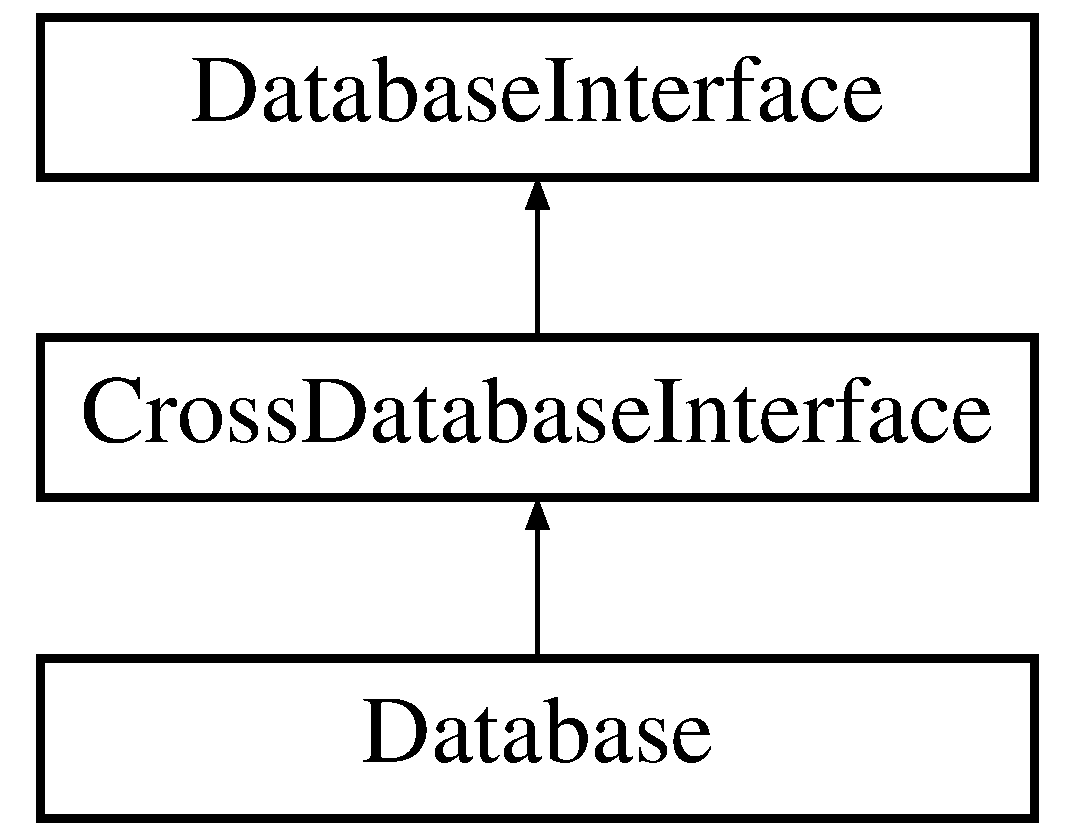
\includegraphics[height=3.000000cm]{interface_cross_database_interface}
\end{center}
\end{figure}
\subsection*{Public Member Functions}
\begin{DoxyCompactItemize}
\item 
\hyperlink{interface_cross_database_interface_ad39d523c1d86281b5776378c1261503d}{\+\_\+\+\_\+construct} (\$type, \$name, \$user=null, \$pass=null, \$host=\textquotesingle{}localhost\textquotesingle{}, \$port=null, \$table=null)
\item 
\hyperlink{interface_cross_database_interface_a42e46ac9d1969ac9ce906608730be110}{get\+Child} ()
\item 
\hyperlink{interface_cross_database_interface_a830b5c75df72b32396701bc563fbe3c7}{get\+Type} ()
\end{DoxyCompactItemize}


\subsection{Detailed Description}


Definition at line 3 of file Cross\+Database\+Interface.\+php.



\subsection{Constructor \& Destructor Documentation}
\hypertarget{interface_cross_database_interface_ad39d523c1d86281b5776378c1261503d}{}\index{Cross\+Database\+Interface@{Cross\+Database\+Interface}!\+\_\+\+\_\+construct@{\+\_\+\+\_\+construct}}
\index{\+\_\+\+\_\+construct@{\+\_\+\+\_\+construct}!Cross\+Database\+Interface@{Cross\+Database\+Interface}}
\subsubsection[{\+\_\+\+\_\+construct}]{\setlength{\rightskip}{0pt plus 5cm}\+\_\+\+\_\+construct (
\begin{DoxyParamCaption}
\item[{}]{\$type, }
\item[{}]{\$name, }
\item[{}]{\$user = {\ttfamily null}, }
\item[{}]{\$pass = {\ttfamily null}, }
\item[{}]{\$host = {\ttfamily \textquotesingle{}localhost\textquotesingle{}}, }
\item[{}]{\$port = {\ttfamily null}, }
\item[{}]{\$table = {\ttfamily null}}
\end{DoxyParamCaption}
)}\label{interface_cross_database_interface_ad39d523c1d86281b5776378c1261503d}


Implemented in \hyperlink{class_database_a8621f88c8cc4a5d71e2856647c086438}{Database}.



\subsection{Member Function Documentation}
\hypertarget{interface_cross_database_interface_a42e46ac9d1969ac9ce906608730be110}{}\index{Cross\+Database\+Interface@{Cross\+Database\+Interface}!get\+Child@{get\+Child}}
\index{get\+Child@{get\+Child}!Cross\+Database\+Interface@{Cross\+Database\+Interface}}
\subsubsection[{get\+Child}]{\setlength{\rightskip}{0pt plus 5cm}get\+Child (
\begin{DoxyParamCaption}
{}
\end{DoxyParamCaption}
)}\label{interface_cross_database_interface_a42e46ac9d1969ac9ce906608730be110}


Implemented in \hyperlink{class_database_a4196f3b1da0c3bbc3ec6f862e2c4e197}{Database}.

\hypertarget{interface_cross_database_interface_a830b5c75df72b32396701bc563fbe3c7}{}\index{Cross\+Database\+Interface@{Cross\+Database\+Interface}!get\+Type@{get\+Type}}
\index{get\+Type@{get\+Type}!Cross\+Database\+Interface@{Cross\+Database\+Interface}}
\subsubsection[{get\+Type}]{\setlength{\rightskip}{0pt plus 5cm}get\+Type (
\begin{DoxyParamCaption}
{}
\end{DoxyParamCaption}
)}\label{interface_cross_database_interface_a830b5c75df72b32396701bc563fbe3c7}


Implemented in \hyperlink{class_database_a830b5c75df72b32396701bc563fbe3c7}{Database}.



The documentation for this interface was generated from the following file\+:\begin{DoxyCompactItemize}
\item 
src/class/\hyperlink{_cross_database_interface_8php}{Cross\+Database\+Interface.\+php}\end{DoxyCompactItemize}

\hypertarget{class_database}{}\section{Database Class Reference}
\label{class_database}\index{Database@{Database}}
Inheritance diagram for Database\+:\begin{figure}[H]
\begin{center}
\leavevmode
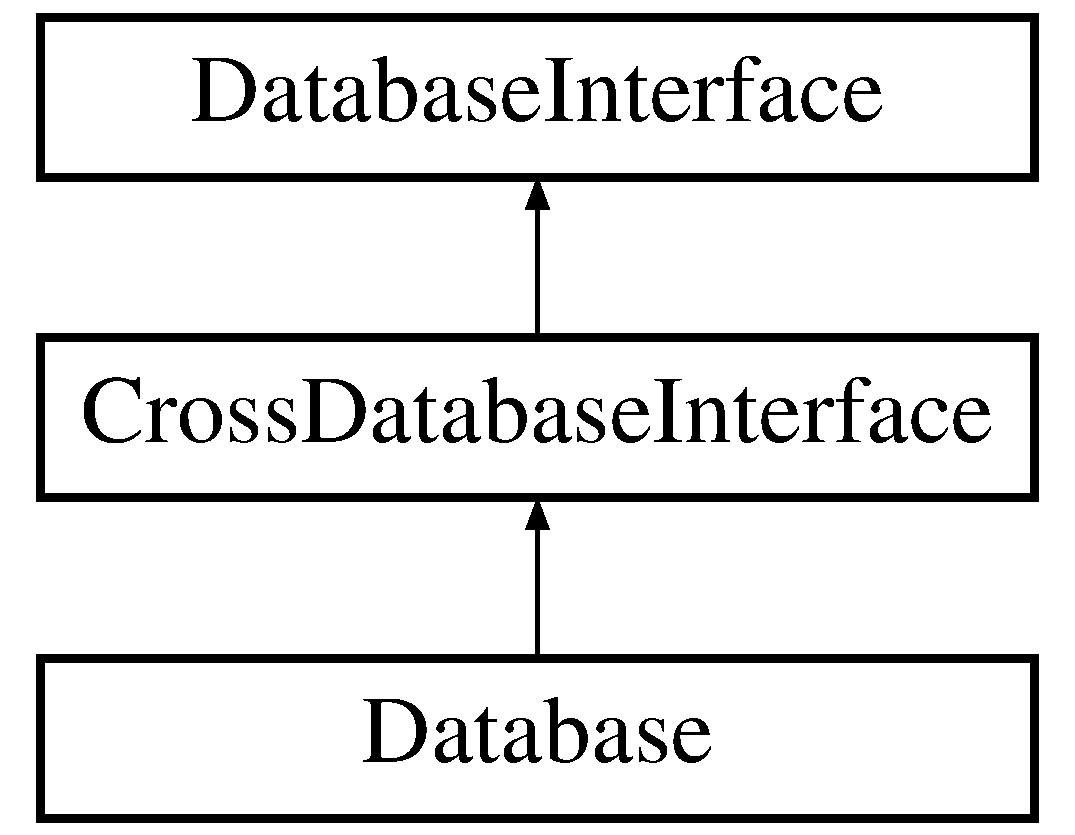
\includegraphics[height=3.000000cm]{class_database}
\end{center}
\end{figure}
\subsection*{Public Member Functions}
\begin{DoxyCompactItemize}
\item 
\hyperlink{class_database_a8621f88c8cc4a5d71e2856647c086438}{\+\_\+\+\_\+construct} (\$type, \$name, \$user=null, \$pass=null, \$host= \textquotesingle{}localhost\textquotesingle{}, \$port=null, \$table=null)
\item 
\hyperlink{class_database_a9aac7e1475efe923de4e19cc2511f092}{\+\_\+\+\_\+invoke} ()
\item 
\hyperlink{class_database_a7516ca30af0db3cdbf9a7739b48ce91d}{\+\_\+\+\_\+to\+String} ()
\item 
\hyperlink{class_database_a42c4cefdb183a7caa3115193a811d893}{column\+Exists} (\$column, \$table=null)
\item 
\& \hyperlink{class_database_a4196f3b1da0c3bbc3ec6f862e2c4e197}{get\+Child} ()
\item 
\hyperlink{class_database_a5cc0962e790b9ccffd2ca9c77cead320}{get\+Columns} (\$table=null)
\item 
\hyperlink{class_database_af54c3eed64c3e3dfb06a2541289ff0da}{get\+Default\+Table} ()
\item 
\hyperlink{class_database_a61b9097ace78236a1a7f9cfd9e9ab01c}{get\+Tables} ()
\item 
\hyperlink{class_database_a830b5c75df72b32396701bc563fbe3c7}{get\+Type} ()
\item 
\hyperlink{class_database_ad0aa1804fc79c22b46596db136320017}{has\+Default\+Table} ()
\item 
\hyperlink{class_database_a8e5626f114925dee9986c8edbfc3ec05}{insert} (\$in, \$table=null)
\item 
\hyperlink{class_database_a1efc6b974510d4c668660f1abe184182}{select} (\$columns=\mbox{[}\textquotesingle{}$\ast$\textquotesingle{}\mbox{]}, \$conditions=null, \$start=null, \$count=null, \$sort\+By=null, \$sort\+Direction=null, \$table=null)
\item 
\hyperlink{class_database_ae7cdaa744d52a1eb0103e377023ca528}{table\+Exists} (\$table)
\end{DoxyCompactItemize}
\subsection*{Data Fields}
\begin{DoxyCompactItemize}
\item 
const \hyperlink{class_database_ac3188f4350978425c488580c5cea8468}{F\+I\+E\+L\+D\+\_\+\+D\+A\+T\+A} = 0
\item 
const \hyperlink{class_database_acbdf154a35cfc228dd1016e8aa4bd503}{F\+I\+E\+L\+D\+\_\+\+T\+A\+B\+L\+E} = 1
\item 
const \hyperlink{class_database_a87aad3e89cc6a17f293cf5410b225bbe}{F\+I\+E\+L\+D\+\_\+\+C\+O\+L\+U\+M\+N} = 2
\item 
const \hyperlink{class_database_a9b1a24ef01d468c146a71b333edb0c17}{K\+E\+Y\+W\+O\+R\+D\+\_\+\+N\+O\+N\+E} = 0
\item 
const \hyperlink{class_database_ababb5c4af464938f3f0b8f9c4fa183ba}{K\+E\+Y\+W\+O\+R\+D\+\_\+\+A\+L\+L} = 1
\item 
const \hyperlink{class_database_af3826c676cb54905f393f9d1f7ad48ea}{S\+O\+R\+T\+\_\+\+N\+O\+N\+E} = 0
\item 
const \hyperlink{class_database_a9517f2622dfc5fbb0cc64feef247eb06}{S\+O\+R\+T\+\_\+\+A\+S\+C} = 1
\item 
const \hyperlink{class_database_a0e633ab431ae1e5cc483a37cfe73bb09}{S\+O\+R\+T\+\_\+\+D\+E\+S\+C} = 2
\item 
const \hyperlink{class_database_ab93424c90d1a3c44eb13221df4a4f773}{T\+Y\+P\+E\+\_\+\+M\+Y\+S\+Q\+L} = 1
\item 
const \hyperlink{class_database_a50a87e8333b1ab093dbeecda41fe4335}{T\+Y\+P\+E\+\_\+\+P\+G\+S\+Q\+L} = 2
\item 
const \hyperlink{class_database_ad651a8cde87b429d4335e15dd6551ca9}{T\+Y\+P\+E\+\_\+\+S\+Q\+L\+I\+T\+E} = 3
\end{DoxyCompactItemize}
\subsection*{Protected Attributes}
\begin{DoxyCompactItemize}
\item 
\hyperlink{class_database_a40410074f5960b0491d35e137147571c}{\$child}
\item 
\hyperlink{class_database_a49c7011be9c979d9174c52a8b83e5d8e}{\$config}
\item 
\hyperlink{class_database_aee271b7ce67fbe00b9976e6c347cbfbf}{\$encoding}
\item 
\hyperlink{class_database_a711797613cb863ca0756df789c396bf2}{\$host}
\item 
\hyperlink{class_database_ab2fc40d43824ea3e1ce5d86dee0d763b}{\$name}
\item 
\hyperlink{class_database_a4269f690c0554ecb1deec21b80f321dc}{\$open}
\item 
\hyperlink{class_database_aa0787efab4b22e8a212882f3409d4c77}{\$port}
\item 
\hyperlink{class_database_ae8876a14058f368335baccf35af4a22b}{\$table}
\item 
\hyperlink{class_database_a9a4a6fba2208984cabb3afacadf33919}{\$type}
\end{DoxyCompactItemize}


\subsection{Detailed Description}


Definition at line 3 of file Database.\+php.



\subsection{Constructor \& Destructor Documentation}
\hypertarget{class_database_a8621f88c8cc4a5d71e2856647c086438}{}\index{Database@{Database}!\+\_\+\+\_\+construct@{\+\_\+\+\_\+construct}}
\index{\+\_\+\+\_\+construct@{\+\_\+\+\_\+construct}!Database@{Database}}
\subsubsection[{\+\_\+\+\_\+construct}]{\setlength{\rightskip}{0pt plus 5cm}\+\_\+\+\_\+construct (
\begin{DoxyParamCaption}
\item[{}]{\$type, }
\item[{}]{\$name, }
\item[{}]{\$user = {\ttfamily null}, }
\item[{}]{\$pass = {\ttfamily null}, }
\item[{}]{\$host = {\ttfamily \textquotesingle{}localhost\textquotesingle{}}, }
\item[{}]{\$port = {\ttfamily null}, }
\item[{}]{\$table = {\ttfamily null}}
\end{DoxyParamCaption}
)}\label{class_database_a8621f88c8cc4a5d71e2856647c086438}
Constructor Method 
\begin{DoxyParams}[1]{Parameters}
int & {\em \$type} & (required) -\/ \\
\hline
string & {\em \$name} & (required) -\/ \\
\hline
string & {\em \$user} & (required for secured) -\/ \\
\hline
string & {\em \$pass} & (required for secured) -\/ \\
\hline
string & {\em \$host} & (required for remote, optional because it defaults to localhost) -\/ \\
\hline
integer & {\em \$port} & (required for remote, optional because it defaults to server type\textquotesingle{}s default port) -\/ \\
\hline
strign & {\em \$table} & (optional) -\/ \\
\hline
\end{DoxyParams}


Implements \hyperlink{interface_cross_database_interface_ad39d523c1d86281b5776378c1261503d}{Cross\+Database\+Interface}.



Definition at line 44 of file Database.\+php.



\subsection{Member Function Documentation}
\hypertarget{class_database_a9aac7e1475efe923de4e19cc2511f092}{}\index{Database@{Database}!\+\_\+\+\_\+invoke@{\+\_\+\+\_\+invoke}}
\index{\+\_\+\+\_\+invoke@{\+\_\+\+\_\+invoke}!Database@{Database}}
\subsubsection[{\+\_\+\+\_\+invoke}]{\setlength{\rightskip}{0pt plus 5cm}\+\_\+\+\_\+invoke (
\begin{DoxyParamCaption}
{}
\end{DoxyParamCaption}
)}\label{class_database_a9aac7e1475efe923de4e19cc2511f092}
Invocation Method 

Implements \hyperlink{interface_database_interface_a9aac7e1475efe923de4e19cc2511f092}{Database\+Interface}.



Definition at line 144 of file Database.\+php.

\hypertarget{class_database_a7516ca30af0db3cdbf9a7739b48ce91d}{}\index{Database@{Database}!\+\_\+\+\_\+to\+String@{\+\_\+\+\_\+to\+String}}
\index{\+\_\+\+\_\+to\+String@{\+\_\+\+\_\+to\+String}!Database@{Database}}
\subsubsection[{\+\_\+\+\_\+to\+String}]{\setlength{\rightskip}{0pt plus 5cm}\+\_\+\+\_\+to\+String (
\begin{DoxyParamCaption}
{}
\end{DoxyParamCaption}
)}\label{class_database_a7516ca30af0db3cdbf9a7739b48ce91d}
String Conversion Method 

Implements \hyperlink{interface_database_interface_a7516ca30af0db3cdbf9a7739b48ce91d}{Database\+Interface}.



Definition at line 153 of file Database.\+php.

\hypertarget{class_database_a42c4cefdb183a7caa3115193a811d893}{}\index{Database@{Database}!column\+Exists@{column\+Exists}}
\index{column\+Exists@{column\+Exists}!Database@{Database}}
\subsubsection[{column\+Exists}]{\setlength{\rightskip}{0pt plus 5cm}column\+Exists (
\begin{DoxyParamCaption}
\item[{}]{\$column, }
\item[{}]{\$table = {\ttfamily null}}
\end{DoxyParamCaption}
)}\label{class_database_a42c4cefdb183a7caa3115193a811d893}
Database-\/$>$\hyperlink{interface_database_interface_a0205d4089913613e23189c60d7fdf89a}{column\+Exists()} Method

Tests if a given column exists in a given table.


\begin{DoxyParams}[1]{Parameters}
string & {\em \$column} & (required) -\/ name of column for which to test \\
\hline
string & {\em \$table} & (optional) -\/ name of table, unless table predefined \\
\hline
\end{DoxyParams}
\begin{DoxyReturn}{Returns}
boolean -\/ true if column exists, false if not 
\end{DoxyReturn}
\begin{DoxySeeAlso}{See also}
\hyperlink{interface_database_interface_a0205d4089913613e23189c60d7fdf89a}{Database\+Interface\+::column\+Exists()} 
\end{DoxySeeAlso}


Definition at line 169 of file Database.\+php.

\hypertarget{class_database_a4196f3b1da0c3bbc3ec6f862e2c4e197}{}\index{Database@{Database}!get\+Child@{get\+Child}}
\index{get\+Child@{get\+Child}!Database@{Database}}
\subsubsection[{get\+Child}]{\setlength{\rightskip}{0pt plus 5cm}\& get\+Child (
\begin{DoxyParamCaption}
{}
\end{DoxyParamCaption}
)}\label{class_database_a4196f3b1da0c3bbc3ec6f862e2c4e197}
Database-\/$>$\hyperlink{class_database_a4196f3b1da0c3bbc3ec6f862e2c4e197}{get\+Child()} Method

Getter for mutable reference to child object (\hyperlink{class_my_s_q_l_database}{My\+S\+Q\+L\+Database}, \hyperlink{class_postgre_s_q_l_database}{Postgre\+S\+Q\+L\+Database}, or \hyperlink{class_s_q_lite_database}{S\+Q\+Lite\+Database}).

\begin{DoxyReturn}{Returns}
\&My\+S\+Q\+L\+Database$\vert$\&Postgre\+S\+Q\+L\+Database$\vert$\&\hyperlink{class_s_q_lite_database}{S\+Q\+Lite\+Database} -\/ child database object 
\end{DoxyReturn}
\begin{DoxySeeAlso}{See also}
\hyperlink{interface_cross_database_interface_a42e46ac9d1969ac9ce906608730be110}{Cross\+Database\+Interface\+::get\+Child()} 
\end{DoxySeeAlso}


Implements \hyperlink{interface_cross_database_interface_a42e46ac9d1969ac9ce906608730be110}{Cross\+Database\+Interface}.



Definition at line 184 of file Database.\+php.

\hypertarget{class_database_a5cc0962e790b9ccffd2ca9c77cead320}{}\index{Database@{Database}!get\+Columns@{get\+Columns}}
\index{get\+Columns@{get\+Columns}!Database@{Database}}
\subsubsection[{get\+Columns}]{\setlength{\rightskip}{0pt plus 5cm}get\+Columns (
\begin{DoxyParamCaption}
\item[{}]{\$table = {\ttfamily null}}
\end{DoxyParamCaption}
)}\label{class_database_a5cc0962e790b9ccffd2ca9c77cead320}
Database-\/$>$\hyperlink{interface_database_interface_a6287262cb9628d7a89d8fc16dcb51177}{get\+Columns()} Method

Getter for array of all columns in a given table.


\begin{DoxyParams}[1]{Parameters}
string & {\em \$table} & (optional) -\/ name of table, unless table predefined \\
\hline
\end{DoxyParams}
\begin{DoxyReturn}{Returns}
array -\/ array of columns in the table 
\end{DoxyReturn}
\begin{DoxySeeAlso}{See also}
\hyperlink{interface_database_interface_a6287262cb9628d7a89d8fc16dcb51177}{Database\+Interface\+::get\+Columns()} 
\end{DoxySeeAlso}


Definition at line 199 of file Database.\+php.

\hypertarget{class_database_af54c3eed64c3e3dfb06a2541289ff0da}{}\index{Database@{Database}!get\+Default\+Table@{get\+Default\+Table}}
\index{get\+Default\+Table@{get\+Default\+Table}!Database@{Database}}
\subsubsection[{get\+Default\+Table}]{\setlength{\rightskip}{0pt plus 5cm}get\+Default\+Table (
\begin{DoxyParamCaption}
{}
\end{DoxyParamCaption}
)}\label{class_database_af54c3eed64c3e3dfb06a2541289ff0da}
Database-\/$>$\hyperlink{class_database_af54c3eed64c3e3dfb06a2541289ff0da}{get\+Default\+Table()} Method

Getter for default table defined in the constructor or Database-\/$>$set\+Table().

\begin{DoxyReturn}{Returns}
string -\/ default table (value of \$this-\/$>$child-\/$>$table) 
\end{DoxyReturn}
\begin{DoxySeeAlso}{See also}
\hyperlink{interface_database_interface_af54c3eed64c3e3dfb06a2541289ff0da}{Database\+Interface\+::get\+Default\+Table()} 
\end{DoxySeeAlso}


Implements \hyperlink{interface_database_interface_af54c3eed64c3e3dfb06a2541289ff0da}{Database\+Interface}.



Definition at line 213 of file Database.\+php.

\hypertarget{class_database_a61b9097ace78236a1a7f9cfd9e9ab01c}{}\index{Database@{Database}!get\+Tables@{get\+Tables}}
\index{get\+Tables@{get\+Tables}!Database@{Database}}
\subsubsection[{get\+Tables}]{\setlength{\rightskip}{0pt plus 5cm}get\+Tables (
\begin{DoxyParamCaption}
{}
\end{DoxyParamCaption}
)}\label{class_database_a61b9097ace78236a1a7f9cfd9e9ab01c}
Database-\/$>$\hyperlink{class_database_a61b9097ace78236a1a7f9cfd9e9ab01c}{get\+Tables()} Method

Getter for array of tables in the database.

\begin{DoxyReturn}{Returns}
array -\/ array of tables in the database 
\end{DoxyReturn}
\begin{DoxySeeAlso}{See also}
\hyperlink{interface_database_interface_a61b9097ace78236a1a7f9cfd9e9ab01c}{Database\+Interface\+::get\+Tables()} 
\end{DoxySeeAlso}


Implements \hyperlink{interface_database_interface_a61b9097ace78236a1a7f9cfd9e9ab01c}{Database\+Interface}.



Definition at line 227 of file Database.\+php.

\hypertarget{class_database_a830b5c75df72b32396701bc563fbe3c7}{}\index{Database@{Database}!get\+Type@{get\+Type}}
\index{get\+Type@{get\+Type}!Database@{Database}}
\subsubsection[{get\+Type}]{\setlength{\rightskip}{0pt plus 5cm}get\+Type (
\begin{DoxyParamCaption}
{}
\end{DoxyParamCaption}
)}\label{class_database_a830b5c75df72b32396701bc563fbe3c7}
Database-\/$>$\hyperlink{class_database_a830b5c75df72b32396701bc563fbe3c7}{get\+Type()} Method

Getter for database type.

\begin{DoxyReturn}{Returns}
string database type, value of \$this-\/$>$type 
\end{DoxyReturn}
\begin{DoxySeeAlso}{See also}
Database\+Interface\+::get\+Type() 
\end{DoxySeeAlso}


Implements \hyperlink{interface_cross_database_interface_a830b5c75df72b32396701bc563fbe3c7}{Cross\+Database\+Interface}.



Definition at line 241 of file Database.\+php.

\hypertarget{class_database_ad0aa1804fc79c22b46596db136320017}{}\index{Database@{Database}!has\+Default\+Table@{has\+Default\+Table}}
\index{has\+Default\+Table@{has\+Default\+Table}!Database@{Database}}
\subsubsection[{has\+Default\+Table}]{\setlength{\rightskip}{0pt plus 5cm}has\+Default\+Table (
\begin{DoxyParamCaption}
{}
\end{DoxyParamCaption}
)}\label{class_database_ad0aa1804fc79c22b46596db136320017}
Database-\/$>$\hyperlink{class_database_ad0aa1804fc79c22b46596db136320017}{has\+Default\+Table()} Method

Checks if default table (defined in constructor or Database-\/$>$set\+Table) is defined.

\begin{DoxyReturn}{Returns}
boolean -\/ true if default table is defined, false if not 
\end{DoxyReturn}
\begin{DoxySeeAlso}{See also}
\hyperlink{interface_database_interface_ad0aa1804fc79c22b46596db136320017}{Database\+Interface\+::has\+Default\+Table()} 
\end{DoxySeeAlso}


Implements \hyperlink{interface_database_interface_ad0aa1804fc79c22b46596db136320017}{Database\+Interface}.



Definition at line 255 of file Database.\+php.

\hypertarget{class_database_a8e5626f114925dee9986c8edbfc3ec05}{}\index{Database@{Database}!insert@{insert}}
\index{insert@{insert}!Database@{Database}}
\subsubsection[{insert}]{\setlength{\rightskip}{0pt plus 5cm}insert (
\begin{DoxyParamCaption}
\item[{}]{\$in, }
\item[{}]{\$table = {\ttfamily null}}
\end{DoxyParamCaption}
)}\label{class_database_a8e5626f114925dee9986c8edbfc3ec05}
Database-\/$>$\hyperlink{class_database_a8e5626f114925dee9986c8edbfc3ec05}{insert()} Method

Insert new data into the database. This method is a chainable mutator.


\begin{DoxyParams}[1]{Parameters}
array & {\em \$in} & (required) -\/ associative array of input to be inserted, keys being the name of columns \\
\hline
string & {\em \$table} & (optional if defined in constructor) -\/ table to use \\
\hline
\end{DoxyParams}
\begin{DoxyReturn}{Returns}
\hyperlink{class_database}{Database} -\/ reference to self 
\end{DoxyReturn}
\begin{DoxySeeAlso}{See also}
\hyperlink{interface_database_interface_a8e5626f114925dee9986c8edbfc3ec05}{Database\+Interface\+::insert()} 
\end{DoxySeeAlso}


Implements \hyperlink{interface_database_interface_a8e5626f114925dee9986c8edbfc3ec05}{Database\+Interface}.



Definition at line 276 of file Database.\+php.

\hypertarget{class_database_a1efc6b974510d4c668660f1abe184182}{}\index{Database@{Database}!select@{select}}
\index{select@{select}!Database@{Database}}
\subsubsection[{select}]{\setlength{\rightskip}{0pt plus 5cm}select (
\begin{DoxyParamCaption}
\item[{}]{\$columns = {\ttfamily \mbox{[}\textquotesingle{}$\ast$\textquotesingle{}\mbox{]}}, }
\item[{}]{\$conditions = {\ttfamily null}, }
\item[{}]{\$start = {\ttfamily null}, }
\item[{}]{\$count = {\ttfamily null}, }
\item[{}]{\$sort\+By = {\ttfamily null}, }
\item[{}]{\$sort\+Direction = {\ttfamily null}, }
\item[{}]{\$table = {\ttfamily null}}
\end{DoxyParamCaption}
)}\label{class_database_a1efc6b974510d4c668660f1abe184182}
Database-\/$>$\hyperlink{class_database_a1efc6b974510d4c668660f1abe184182}{select()} Method


\begin{DoxyParams}[1]{Parameters}
array | string & {\em \$columns} & (optional) -\/ columns to return. if left empty/null, will default to all columns ($\ast$) \\
\hline
Database\+Condition | array | string & {\em \$conditions} & (optional) -\/ conditions to lookup. If left empty/null, will default to no conditions. \\
\hline
int & {\em \$start} & (optional) -\/ starting index from which to begin selecting. If left empty, defaults to 0. \\
\hline
int & {\em \$count} & (optional) -\/ maximum number of results to return. If left empty, defaults to no limit. \\
\hline
string & {\em \$sort\+By} & (optional) -\/ column with which to sort the table. If left empty, defaults to the first column in the table. \\
\hline
int & {\em \$sort\+Direction} & (optional -\/ (uses flags) direction to sort the table. If left empty, defaults to none. Options are S\+O\+R\+T\+\_\+\+N\+O\+N\+E, S\+O\+R\+T\+\_\+\+A\+S\+C, S\+O\+R\+T\+\_\+\+D\+E\+S\+C \\
\hline
string & {\em \$table} & (optional if table set in constructor) -\/ table from which to select. \\
\hline
\end{DoxyParams}
\begin{DoxyReturn}{Returns}
array -\/ results of the select query as an associative array. 
\end{DoxyReturn}


Implements \hyperlink{interface_database_interface_a1efc6b974510d4c668660f1abe184182}{Database\+Interface}.



Definition at line 294 of file Database.\+php.

\hypertarget{class_database_ae7cdaa744d52a1eb0103e377023ca528}{}\index{Database@{Database}!table\+Exists@{table\+Exists}}
\index{table\+Exists@{table\+Exists}!Database@{Database}}
\subsubsection[{table\+Exists}]{\setlength{\rightskip}{0pt plus 5cm}table\+Exists (
\begin{DoxyParamCaption}
\item[{}]{\$table}
\end{DoxyParamCaption}
)}\label{class_database_ae7cdaa744d52a1eb0103e377023ca528}
Database-\/$>$\hyperlink{class_database_ae7cdaa744d52a1eb0103e377023ca528}{table\+Exists()} Method

Checks if a given table exists in the database


\begin{DoxyParams}[1]{Parameters}
string & {\em \$table} & (required) -\/ table for which to check \\
\hline
\end{DoxyParams}
\begin{DoxyReturn}{Returns}
boolean -\/ true if table exists, false if not 
\end{DoxyReturn}
\begin{DoxySeeAlso}{See also}
\hyperlink{interface_database_interface_ae7cdaa744d52a1eb0103e377023ca528}{Database\+Interface\+::table\+Exists()} 
\end{DoxySeeAlso}


Implements \hyperlink{interface_database_interface_ae7cdaa744d52a1eb0103e377023ca528}{Database\+Interface}.



Definition at line 309 of file Database.\+php.



\subsection{Field Documentation}
\hypertarget{class_database_a40410074f5960b0491d35e137147571c}{}\index{Database@{Database}!\$child@{\$child}}
\index{\$child@{\$child}!Database@{Database}}
\subsubsection[{\$child}]{\setlength{\rightskip}{0pt plus 5cm}\$child\hspace{0.3cm}{\ttfamily [protected]}}\label{class_database_a40410074f5960b0491d35e137147571c}


Definition at line 7 of file Database.\+php.

\hypertarget{class_database_a49c7011be9c979d9174c52a8b83e5d8e}{}\index{Database@{Database}!\$config@{\$config}}
\index{\$config@{\$config}!Database@{Database}}
\subsubsection[{\$config}]{\setlength{\rightskip}{0pt plus 5cm}\$config\hspace{0.3cm}{\ttfamily [protected]}}\label{class_database_a49c7011be9c979d9174c52a8b83e5d8e}


Definition at line 8 of file Database.\+php.

\hypertarget{class_database_aee271b7ce67fbe00b9976e6c347cbfbf}{}\index{Database@{Database}!\$encoding@{\$encoding}}
\index{\$encoding@{\$encoding}!Database@{Database}}
\subsubsection[{\$encoding}]{\setlength{\rightskip}{0pt plus 5cm}\$encoding\hspace{0.3cm}{\ttfamily [protected]}}\label{class_database_aee271b7ce67fbe00b9976e6c347cbfbf}


Definition at line 9 of file Database.\+php.

\hypertarget{class_database_a711797613cb863ca0756df789c396bf2}{}\index{Database@{Database}!\$host@{\$host}}
\index{\$host@{\$host}!Database@{Database}}
\subsubsection[{\$host}]{\setlength{\rightskip}{0pt plus 5cm}\$host\hspace{0.3cm}{\ttfamily [protected]}}\label{class_database_a711797613cb863ca0756df789c396bf2}


Definition at line 10 of file Database.\+php.

\hypertarget{class_database_ab2fc40d43824ea3e1ce5d86dee0d763b}{}\index{Database@{Database}!\$name@{\$name}}
\index{\$name@{\$name}!Database@{Database}}
\subsubsection[{\$name}]{\setlength{\rightskip}{0pt plus 5cm}\$name\hspace{0.3cm}{\ttfamily [protected]}}\label{class_database_ab2fc40d43824ea3e1ce5d86dee0d763b}


Definition at line 11 of file Database.\+php.

\hypertarget{class_database_a4269f690c0554ecb1deec21b80f321dc}{}\index{Database@{Database}!\$open@{\$open}}
\index{\$open@{\$open}!Database@{Database}}
\subsubsection[{\$open}]{\setlength{\rightskip}{0pt plus 5cm}\$open\hspace{0.3cm}{\ttfamily [protected]}}\label{class_database_a4269f690c0554ecb1deec21b80f321dc}


Definition at line 12 of file Database.\+php.

\hypertarget{class_database_aa0787efab4b22e8a212882f3409d4c77}{}\index{Database@{Database}!\$port@{\$port}}
\index{\$port@{\$port}!Database@{Database}}
\subsubsection[{\$port}]{\setlength{\rightskip}{0pt plus 5cm}\$port\hspace{0.3cm}{\ttfamily [protected]}}\label{class_database_aa0787efab4b22e8a212882f3409d4c77}


Definition at line 13 of file Database.\+php.

\hypertarget{class_database_ae8876a14058f368335baccf35af4a22b}{}\index{Database@{Database}!\$table@{\$table}}
\index{\$table@{\$table}!Database@{Database}}
\subsubsection[{\$table}]{\setlength{\rightskip}{0pt plus 5cm}\$table\hspace{0.3cm}{\ttfamily [protected]}}\label{class_database_ae8876a14058f368335baccf35af4a22b}


Definition at line 14 of file Database.\+php.

\hypertarget{class_database_a9a4a6fba2208984cabb3afacadf33919}{}\index{Database@{Database}!\$type@{\$type}}
\index{\$type@{\$type}!Database@{Database}}
\subsubsection[{\$type}]{\setlength{\rightskip}{0pt plus 5cm}\$type\hspace{0.3cm}{\ttfamily [protected]}}\label{class_database_a9a4a6fba2208984cabb3afacadf33919}


Definition at line 15 of file Database.\+php.

\hypertarget{class_database_a87aad3e89cc6a17f293cf5410b225bbe}{}\index{Database@{Database}!F\+I\+E\+L\+D\+\_\+\+C\+O\+L\+U\+M\+N@{F\+I\+E\+L\+D\+\_\+\+C\+O\+L\+U\+M\+N}}
\index{F\+I\+E\+L\+D\+\_\+\+C\+O\+L\+U\+M\+N@{F\+I\+E\+L\+D\+\_\+\+C\+O\+L\+U\+M\+N}!Database@{Database}}
\subsubsection[{F\+I\+E\+L\+D\+\_\+\+C\+O\+L\+U\+M\+N}]{\setlength{\rightskip}{0pt plus 5cm}const F\+I\+E\+L\+D\+\_\+\+C\+O\+L\+U\+M\+N = 2}\label{class_database_a87aad3e89cc6a17f293cf5410b225bbe}


Definition at line 21 of file Database.\+php.

\hypertarget{class_database_ac3188f4350978425c488580c5cea8468}{}\index{Database@{Database}!F\+I\+E\+L\+D\+\_\+\+D\+A\+T\+A@{F\+I\+E\+L\+D\+\_\+\+D\+A\+T\+A}}
\index{F\+I\+E\+L\+D\+\_\+\+D\+A\+T\+A@{F\+I\+E\+L\+D\+\_\+\+D\+A\+T\+A}!Database@{Database}}
\subsubsection[{F\+I\+E\+L\+D\+\_\+\+D\+A\+T\+A}]{\setlength{\rightskip}{0pt plus 5cm}const F\+I\+E\+L\+D\+\_\+\+D\+A\+T\+A = 0}\label{class_database_ac3188f4350978425c488580c5cea8468}


Definition at line 19 of file Database.\+php.

\hypertarget{class_database_acbdf154a35cfc228dd1016e8aa4bd503}{}\index{Database@{Database}!F\+I\+E\+L\+D\+\_\+\+T\+A\+B\+L\+E@{F\+I\+E\+L\+D\+\_\+\+T\+A\+B\+L\+E}}
\index{F\+I\+E\+L\+D\+\_\+\+T\+A\+B\+L\+E@{F\+I\+E\+L\+D\+\_\+\+T\+A\+B\+L\+E}!Database@{Database}}
\subsubsection[{F\+I\+E\+L\+D\+\_\+\+T\+A\+B\+L\+E}]{\setlength{\rightskip}{0pt plus 5cm}const F\+I\+E\+L\+D\+\_\+\+T\+A\+B\+L\+E = 1}\label{class_database_acbdf154a35cfc228dd1016e8aa4bd503}


Definition at line 20 of file Database.\+php.

\hypertarget{class_database_ababb5c4af464938f3f0b8f9c4fa183ba}{}\index{Database@{Database}!K\+E\+Y\+W\+O\+R\+D\+\_\+\+A\+L\+L@{K\+E\+Y\+W\+O\+R\+D\+\_\+\+A\+L\+L}}
\index{K\+E\+Y\+W\+O\+R\+D\+\_\+\+A\+L\+L@{K\+E\+Y\+W\+O\+R\+D\+\_\+\+A\+L\+L}!Database@{Database}}
\subsubsection[{K\+E\+Y\+W\+O\+R\+D\+\_\+\+A\+L\+L}]{\setlength{\rightskip}{0pt plus 5cm}const K\+E\+Y\+W\+O\+R\+D\+\_\+\+A\+L\+L = 1}\label{class_database_ababb5c4af464938f3f0b8f9c4fa183ba}


Definition at line 24 of file Database.\+php.

\hypertarget{class_database_a9b1a24ef01d468c146a71b333edb0c17}{}\index{Database@{Database}!K\+E\+Y\+W\+O\+R\+D\+\_\+\+N\+O\+N\+E@{K\+E\+Y\+W\+O\+R\+D\+\_\+\+N\+O\+N\+E}}
\index{K\+E\+Y\+W\+O\+R\+D\+\_\+\+N\+O\+N\+E@{K\+E\+Y\+W\+O\+R\+D\+\_\+\+N\+O\+N\+E}!Database@{Database}}
\subsubsection[{K\+E\+Y\+W\+O\+R\+D\+\_\+\+N\+O\+N\+E}]{\setlength{\rightskip}{0pt plus 5cm}const K\+E\+Y\+W\+O\+R\+D\+\_\+\+N\+O\+N\+E = 0}\label{class_database_a9b1a24ef01d468c146a71b333edb0c17}


Definition at line 23 of file Database.\+php.

\hypertarget{class_database_a9517f2622dfc5fbb0cc64feef247eb06}{}\index{Database@{Database}!S\+O\+R\+T\+\_\+\+A\+S\+C@{S\+O\+R\+T\+\_\+\+A\+S\+C}}
\index{S\+O\+R\+T\+\_\+\+A\+S\+C@{S\+O\+R\+T\+\_\+\+A\+S\+C}!Database@{Database}}
\subsubsection[{S\+O\+R\+T\+\_\+\+A\+S\+C}]{\setlength{\rightskip}{0pt plus 5cm}const S\+O\+R\+T\+\_\+\+A\+S\+C = 1}\label{class_database_a9517f2622dfc5fbb0cc64feef247eb06}


Definition at line 27 of file Database.\+php.

\hypertarget{class_database_a0e633ab431ae1e5cc483a37cfe73bb09}{}\index{Database@{Database}!S\+O\+R\+T\+\_\+\+D\+E\+S\+C@{S\+O\+R\+T\+\_\+\+D\+E\+S\+C}}
\index{S\+O\+R\+T\+\_\+\+D\+E\+S\+C@{S\+O\+R\+T\+\_\+\+D\+E\+S\+C}!Database@{Database}}
\subsubsection[{S\+O\+R\+T\+\_\+\+D\+E\+S\+C}]{\setlength{\rightskip}{0pt plus 5cm}const S\+O\+R\+T\+\_\+\+D\+E\+S\+C = 2}\label{class_database_a0e633ab431ae1e5cc483a37cfe73bb09}


Definition at line 28 of file Database.\+php.

\hypertarget{class_database_af3826c676cb54905f393f9d1f7ad48ea}{}\index{Database@{Database}!S\+O\+R\+T\+\_\+\+N\+O\+N\+E@{S\+O\+R\+T\+\_\+\+N\+O\+N\+E}}
\index{S\+O\+R\+T\+\_\+\+N\+O\+N\+E@{S\+O\+R\+T\+\_\+\+N\+O\+N\+E}!Database@{Database}}
\subsubsection[{S\+O\+R\+T\+\_\+\+N\+O\+N\+E}]{\setlength{\rightskip}{0pt plus 5cm}const S\+O\+R\+T\+\_\+\+N\+O\+N\+E = 0}\label{class_database_af3826c676cb54905f393f9d1f7ad48ea}


Definition at line 26 of file Database.\+php.

\hypertarget{class_database_ab93424c90d1a3c44eb13221df4a4f773}{}\index{Database@{Database}!T\+Y\+P\+E\+\_\+\+M\+Y\+S\+Q\+L@{T\+Y\+P\+E\+\_\+\+M\+Y\+S\+Q\+L}}
\index{T\+Y\+P\+E\+\_\+\+M\+Y\+S\+Q\+L@{T\+Y\+P\+E\+\_\+\+M\+Y\+S\+Q\+L}!Database@{Database}}
\subsubsection[{T\+Y\+P\+E\+\_\+\+M\+Y\+S\+Q\+L}]{\setlength{\rightskip}{0pt plus 5cm}const T\+Y\+P\+E\+\_\+\+M\+Y\+S\+Q\+L = 1}\label{class_database_ab93424c90d1a3c44eb13221df4a4f773}


Definition at line 30 of file Database.\+php.

\hypertarget{class_database_a50a87e8333b1ab093dbeecda41fe4335}{}\index{Database@{Database}!T\+Y\+P\+E\+\_\+\+P\+G\+S\+Q\+L@{T\+Y\+P\+E\+\_\+\+P\+G\+S\+Q\+L}}
\index{T\+Y\+P\+E\+\_\+\+P\+G\+S\+Q\+L@{T\+Y\+P\+E\+\_\+\+P\+G\+S\+Q\+L}!Database@{Database}}
\subsubsection[{T\+Y\+P\+E\+\_\+\+P\+G\+S\+Q\+L}]{\setlength{\rightskip}{0pt plus 5cm}const T\+Y\+P\+E\+\_\+\+P\+G\+S\+Q\+L = 2}\label{class_database_a50a87e8333b1ab093dbeecda41fe4335}


Definition at line 31 of file Database.\+php.

\hypertarget{class_database_ad651a8cde87b429d4335e15dd6551ca9}{}\index{Database@{Database}!T\+Y\+P\+E\+\_\+\+S\+Q\+L\+I\+T\+E@{T\+Y\+P\+E\+\_\+\+S\+Q\+L\+I\+T\+E}}
\index{T\+Y\+P\+E\+\_\+\+S\+Q\+L\+I\+T\+E@{T\+Y\+P\+E\+\_\+\+S\+Q\+L\+I\+T\+E}!Database@{Database}}
\subsubsection[{T\+Y\+P\+E\+\_\+\+S\+Q\+L\+I\+T\+E}]{\setlength{\rightskip}{0pt plus 5cm}const T\+Y\+P\+E\+\_\+\+S\+Q\+L\+I\+T\+E = 3}\label{class_database_ad651a8cde87b429d4335e15dd6551ca9}


Definition at line 32 of file Database.\+php.



The documentation for this class was generated from the following file\+:\begin{DoxyCompactItemize}
\item 
src/class/\hyperlink{_database_8php}{Database.\+php}\end{DoxyCompactItemize}

\hypertarget{interface_database_condition_interface}{}\section{Database\+Condition\+Interface Interface Reference}
\label{interface_database_condition_interface}\index{Database\+Condition\+Interface@{Database\+Condition\+Interface}}
Inheritance diagram for Database\+Condition\+Interface\+:\begin{figure}[H]
\begin{center}
\leavevmode
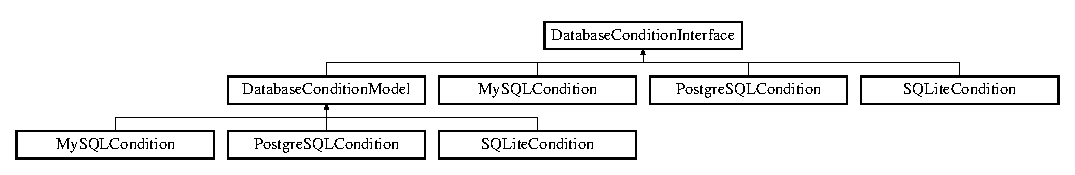
\includegraphics[height=1.909091cm]{interface_database_condition_interface}
\end{center}
\end{figure}
\subsection*{Public Member Functions}
\begin{DoxyCompactItemize}
\item 
\hyperlink{interface_database_condition_interface_aeb576c3b33394f5ab4f37c7e64d44502}{\+\_\+\+\_\+construct} (\$struct=\mbox{[}$\,$\mbox{]})
\item 
\hyperlink{interface_database_condition_interface_a9aac7e1475efe923de4e19cc2511f092}{\+\_\+\+\_\+invoke} ()
\item 
\hyperlink{interface_database_condition_interface_a7516ca30af0db3cdbf9a7739b48ce91d}{\+\_\+\+\_\+to\+String} ()
\item 
\hyperlink{interface_database_condition_interface_a8fe63e52baa6d003a96482ee5068abe5}{array\+Parse} (array \$array, \$encap=false)
\item 
\hyperlink{interface_database_condition_interface_a71922b66dbbd931e3bd73bd0b8c6bc0f}{get\+Statement} ()
\item 
\hyperlink{interface_database_condition_interface_ac039a7d66b72b41cbc80f4507d254f68}{get\+Structure} ()
\item 
\hyperlink{interface_database_condition_interface_a0746ee466ee9178068496aa443ed9189}{insert} (\$array)
\item 
\hyperlink{interface_database_condition_interface_a170962f6550bf5cefcf4a871dcebc25e}{remove} (\$array)
\end{DoxyCompactItemize}


\subsection{Detailed Description}


Definition at line 3 of file Database\+Condition\+Interface.\+php.



\subsection{Constructor \& Destructor Documentation}
\hypertarget{interface_database_condition_interface_aeb576c3b33394f5ab4f37c7e64d44502}{}\index{Database\+Condition\+Interface@{Database\+Condition\+Interface}!\+\_\+\+\_\+construct@{\+\_\+\+\_\+construct}}
\index{\+\_\+\+\_\+construct@{\+\_\+\+\_\+construct}!Database\+Condition\+Interface@{Database\+Condition\+Interface}}
\subsubsection[{\+\_\+\+\_\+construct}]{\setlength{\rightskip}{0pt plus 5cm}\+\_\+\+\_\+construct (
\begin{DoxyParamCaption}
\item[{}]{\$struct = {\ttfamily \mbox{[}\mbox{]}}}
\end{DoxyParamCaption}
)}\label{interface_database_condition_interface_aeb576c3b33394f5ab4f37c7e64d44502}


Implemented in \hyperlink{class_database_condition_model_aeb576c3b33394f5ab4f37c7e64d44502}{Database\+Condition\+Model}.



\subsection{Member Function Documentation}
\hypertarget{interface_database_condition_interface_a9aac7e1475efe923de4e19cc2511f092}{}\index{Database\+Condition\+Interface@{Database\+Condition\+Interface}!\+\_\+\+\_\+invoke@{\+\_\+\+\_\+invoke}}
\index{\+\_\+\+\_\+invoke@{\+\_\+\+\_\+invoke}!Database\+Condition\+Interface@{Database\+Condition\+Interface}}
\subsubsection[{\+\_\+\+\_\+invoke}]{\setlength{\rightskip}{0pt plus 5cm}\+\_\+\+\_\+invoke (
\begin{DoxyParamCaption}
{}
\end{DoxyParamCaption}
)}\label{interface_database_condition_interface_a9aac7e1475efe923de4e19cc2511f092}


Implemented in \hyperlink{class_database_condition_model_a9aac7e1475efe923de4e19cc2511f092}{Database\+Condition\+Model}.

\hypertarget{interface_database_condition_interface_a7516ca30af0db3cdbf9a7739b48ce91d}{}\index{Database\+Condition\+Interface@{Database\+Condition\+Interface}!\+\_\+\+\_\+to\+String@{\+\_\+\+\_\+to\+String}}
\index{\+\_\+\+\_\+to\+String@{\+\_\+\+\_\+to\+String}!Database\+Condition\+Interface@{Database\+Condition\+Interface}}
\subsubsection[{\+\_\+\+\_\+to\+String}]{\setlength{\rightskip}{0pt plus 5cm}\+\_\+\+\_\+to\+String (
\begin{DoxyParamCaption}
{}
\end{DoxyParamCaption}
)}\label{interface_database_condition_interface_a7516ca30af0db3cdbf9a7739b48ce91d}


Implemented in \hyperlink{class_database_condition_model_a7516ca30af0db3cdbf9a7739b48ce91d}{Database\+Condition\+Model}.

\hypertarget{interface_database_condition_interface_a8fe63e52baa6d003a96482ee5068abe5}{}\index{Database\+Condition\+Interface@{Database\+Condition\+Interface}!array\+Parse@{array\+Parse}}
\index{array\+Parse@{array\+Parse}!Database\+Condition\+Interface@{Database\+Condition\+Interface}}
\subsubsection[{array\+Parse}]{\setlength{\rightskip}{0pt plus 5cm}array\+Parse (
\begin{DoxyParamCaption}
\item[{array}]{\$array, }
\item[{}]{\$encap = {\ttfamily false}}
\end{DoxyParamCaption}
)}\label{interface_database_condition_interface_a8fe63e52baa6d003a96482ee5068abe5}


Implemented in \hyperlink{class_database_condition_model_afb03c211ff377a7d956b746d1331ad60}{Database\+Condition\+Model}.

\hypertarget{interface_database_condition_interface_a71922b66dbbd931e3bd73bd0b8c6bc0f}{}\index{Database\+Condition\+Interface@{Database\+Condition\+Interface}!get\+Statement@{get\+Statement}}
\index{get\+Statement@{get\+Statement}!Database\+Condition\+Interface@{Database\+Condition\+Interface}}
\subsubsection[{get\+Statement}]{\setlength{\rightskip}{0pt plus 5cm}get\+Statement (
\begin{DoxyParamCaption}
{}
\end{DoxyParamCaption}
)}\label{interface_database_condition_interface_a71922b66dbbd931e3bd73bd0b8c6bc0f}


Implemented in \hyperlink{class_database_condition_model_a71922b66dbbd931e3bd73bd0b8c6bc0f}{Database\+Condition\+Model}.

\hypertarget{interface_database_condition_interface_ac039a7d66b72b41cbc80f4507d254f68}{}\index{Database\+Condition\+Interface@{Database\+Condition\+Interface}!get\+Structure@{get\+Structure}}
\index{get\+Structure@{get\+Structure}!Database\+Condition\+Interface@{Database\+Condition\+Interface}}
\subsubsection[{get\+Structure}]{\setlength{\rightskip}{0pt plus 5cm}get\+Structure (
\begin{DoxyParamCaption}
{}
\end{DoxyParamCaption}
)}\label{interface_database_condition_interface_ac039a7d66b72b41cbc80f4507d254f68}


Implemented in \hyperlink{class_database_condition_model_ac039a7d66b72b41cbc80f4507d254f68}{Database\+Condition\+Model}.

\hypertarget{interface_database_condition_interface_a0746ee466ee9178068496aa443ed9189}{}\index{Database\+Condition\+Interface@{Database\+Condition\+Interface}!insert@{insert}}
\index{insert@{insert}!Database\+Condition\+Interface@{Database\+Condition\+Interface}}
\subsubsection[{insert}]{\setlength{\rightskip}{0pt plus 5cm}insert (
\begin{DoxyParamCaption}
\item[{}]{\$array}
\end{DoxyParamCaption}
)}\label{interface_database_condition_interface_a0746ee466ee9178068496aa443ed9189}


Implemented in \hyperlink{class_database_condition_model_a0746ee466ee9178068496aa443ed9189}{Database\+Condition\+Model}.

\hypertarget{interface_database_condition_interface_a170962f6550bf5cefcf4a871dcebc25e}{}\index{Database\+Condition\+Interface@{Database\+Condition\+Interface}!remove@{remove}}
\index{remove@{remove}!Database\+Condition\+Interface@{Database\+Condition\+Interface}}
\subsubsection[{remove}]{\setlength{\rightskip}{0pt plus 5cm}remove (
\begin{DoxyParamCaption}
\item[{}]{\$array}
\end{DoxyParamCaption}
)}\label{interface_database_condition_interface_a170962f6550bf5cefcf4a871dcebc25e}


Implemented in \hyperlink{class_database_condition_model_a170962f6550bf5cefcf4a871dcebc25e}{Database\+Condition\+Model}.



The documentation for this interface was generated from the following file\+:\begin{DoxyCompactItemize}
\item 
src/class/\hyperlink{_database_condition_interface_8php}{Database\+Condition\+Interface.\+php}\end{DoxyCompactItemize}

\hypertarget{class_database_condition_model}{}\section{Database\+Condition\+Model Class Reference}
\label{class_database_condition_model}\index{Database\+Condition\+Model@{Database\+Condition\+Model}}
Inheritance diagram for Database\+Condition\+Model\+:\begin{figure}[H]
\begin{center}
\leavevmode
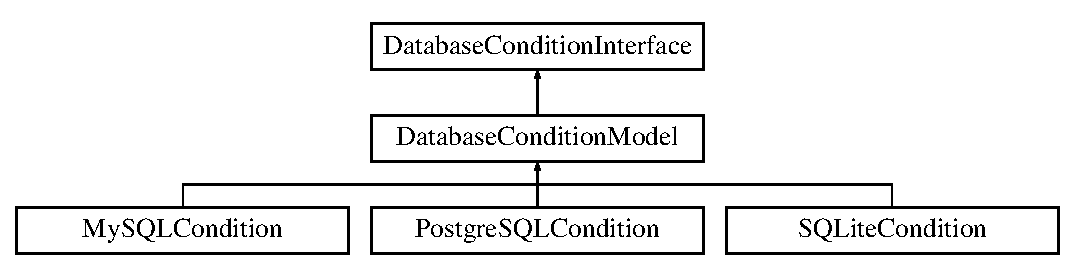
\includegraphics[height=3.000000cm]{class_database_condition_model}
\end{center}
\end{figure}
\subsection*{Public Member Functions}
\begin{DoxyCompactItemize}
\item 
\hyperlink{class_database_condition_model_aeb576c3b33394f5ab4f37c7e64d44502}{\+\_\+\+\_\+construct} (\$struct=\mbox{[}$\,$\mbox{]})
\item 
\hyperlink{class_database_condition_model_a421831a265621325e1fdd19aace0c758}{\+\_\+\+\_\+destruct} ()
\item 
\hyperlink{class_database_condition_model_a9aac7e1475efe923de4e19cc2511f092}{\+\_\+\+\_\+invoke} ()
\item 
\hyperlink{class_database_condition_model_a7516ca30af0db3cdbf9a7739b48ce91d}{\+\_\+\+\_\+to\+String} ()
\item 
\hyperlink{class_database_condition_model_a069b0ea1d8bcd11e99e5e2e2076841ff}{fresh} (\$array)
\item 
\hyperlink{class_database_condition_model_a71922b66dbbd931e3bd73bd0b8c6bc0f}{get\+Statement} ()
\item 
\hyperlink{class_database_condition_model_ac039a7d66b72b41cbc80f4507d254f68}{get\+Structure} ()
\item 
\hyperlink{class_database_condition_model_a0746ee466ee9178068496aa443ed9189}{insert} (\$array)
\item 
\hyperlink{class_database_condition_model_a170962f6550bf5cefcf4a871dcebc25e}{remove} (\$array)
\end{DoxyCompactItemize}
\subsection*{Static Public Member Functions}
\begin{DoxyCompactItemize}
\item 
static \hyperlink{class_database_condition_model_afb03c211ff377a7d956b746d1331ad60}{array\+Parse} (array \$array, \$encap=false)
\end{DoxyCompactItemize}
\subsection*{Protected Attributes}
\begin{DoxyCompactItemize}
\item 
\hyperlink{class_database_condition_model_a776dc234d8e2b257550d9444ddf5d399}{\$statement} = \mbox{[}$\,$\mbox{]}
\item 
\hyperlink{class_database_condition_model_aa78d61fba96a50ae36cf20c6de2b8e64}{\$structure} = \mbox{[}$\,$\mbox{]}
\end{DoxyCompactItemize}


\subsection{Detailed Description}


Definition at line 3 of file Database\+Condition\+Model.\+php.



\subsection{Constructor \& Destructor Documentation}
\hypertarget{class_database_condition_model_aeb576c3b33394f5ab4f37c7e64d44502}{}\index{Database\+Condition\+Model@{Database\+Condition\+Model}!\+\_\+\+\_\+construct@{\+\_\+\+\_\+construct}}
\index{\+\_\+\+\_\+construct@{\+\_\+\+\_\+construct}!Database\+Condition\+Model@{Database\+Condition\+Model}}
\subsubsection[{\+\_\+\+\_\+construct}]{\setlength{\rightskip}{0pt plus 5cm}\+\_\+\+\_\+construct (
\begin{DoxyParamCaption}
\item[{}]{\$struct = {\ttfamily \mbox{[}\mbox{]}}}
\end{DoxyParamCaption}
)}\label{class_database_condition_model_aeb576c3b33394f5ab4f37c7e64d44502}
Constructor Method 
\begin{DoxyParams}[1]{Parameters}
unknown & {\em \$struct} & \\
\hline
\end{DoxyParams}


Implements \hyperlink{interface_database_condition_interface_aeb576c3b33394f5ab4f37c7e64d44502}{Database\+Condition\+Interface}.



Definition at line 12 of file Database\+Condition\+Model.\+php.

\hypertarget{class_database_condition_model_a421831a265621325e1fdd19aace0c758}{}\index{Database\+Condition\+Model@{Database\+Condition\+Model}!\+\_\+\+\_\+destruct@{\+\_\+\+\_\+destruct}}
\index{\+\_\+\+\_\+destruct@{\+\_\+\+\_\+destruct}!Database\+Condition\+Model@{Database\+Condition\+Model}}
\subsubsection[{\+\_\+\+\_\+destruct}]{\setlength{\rightskip}{0pt plus 5cm}\+\_\+\+\_\+destruct (
\begin{DoxyParamCaption}
{}
\end{DoxyParamCaption}
)}\label{class_database_condition_model_a421831a265621325e1fdd19aace0c758}


Definition at line 19 of file Database\+Condition\+Model.\+php.



\subsection{Member Function Documentation}
\hypertarget{class_database_condition_model_a9aac7e1475efe923de4e19cc2511f092}{}\index{Database\+Condition\+Model@{Database\+Condition\+Model}!\+\_\+\+\_\+invoke@{\+\_\+\+\_\+invoke}}
\index{\+\_\+\+\_\+invoke@{\+\_\+\+\_\+invoke}!Database\+Condition\+Model@{Database\+Condition\+Model}}
\subsubsection[{\+\_\+\+\_\+invoke}]{\setlength{\rightskip}{0pt plus 5cm}\+\_\+\+\_\+invoke (
\begin{DoxyParamCaption}
{}
\end{DoxyParamCaption}
)}\label{class_database_condition_model_a9aac7e1475efe923de4e19cc2511f092}


Implements \hyperlink{interface_database_condition_interface_a9aac7e1475efe923de4e19cc2511f092}{Database\+Condition\+Interface}.



Definition at line 25 of file Database\+Condition\+Model.\+php.

\hypertarget{class_database_condition_model_a7516ca30af0db3cdbf9a7739b48ce91d}{}\index{Database\+Condition\+Model@{Database\+Condition\+Model}!\+\_\+\+\_\+to\+String@{\+\_\+\+\_\+to\+String}}
\index{\+\_\+\+\_\+to\+String@{\+\_\+\+\_\+to\+String}!Database\+Condition\+Model@{Database\+Condition\+Model}}
\subsubsection[{\+\_\+\+\_\+to\+String}]{\setlength{\rightskip}{0pt plus 5cm}\+\_\+\+\_\+to\+String (
\begin{DoxyParamCaption}
{}
\end{DoxyParamCaption}
)}\label{class_database_condition_model_a7516ca30af0db3cdbf9a7739b48ce91d}


Implements \hyperlink{interface_database_condition_interface_a7516ca30af0db3cdbf9a7739b48ce91d}{Database\+Condition\+Interface}.



Definition at line 31 of file Database\+Condition\+Model.\+php.

\hypertarget{class_database_condition_model_afb03c211ff377a7d956b746d1331ad60}{}\index{Database\+Condition\+Model@{Database\+Condition\+Model}!array\+Parse@{array\+Parse}}
\index{array\+Parse@{array\+Parse}!Database\+Condition\+Model@{Database\+Condition\+Model}}
\subsubsection[{array\+Parse}]{\setlength{\rightskip}{0pt plus 5cm}static array\+Parse (
\begin{DoxyParamCaption}
\item[{array}]{\$array, }
\item[{}]{\$encap = {\ttfamily false}}
\end{DoxyParamCaption}
)\hspace{0.3cm}{\ttfamily [static]}}\label{class_database_condition_model_afb03c211ff377a7d956b746d1331ad60}
\hyperlink{class_database_condition_model_afb03c211ff377a7d956b746d1331ad60}{Database\+Condition\+Model\+::array\+Parse()} Static Method

Converts an associative array of S\+Q\+L boolean logic conditions to a string that can be used in a standard S\+Q\+L query.


\begin{DoxyParams}[1]{Parameters}
array & {\em \$array} & \\
\hline
bool & {\em \$encap} & \\
\hline
\end{DoxyParams}
\begin{DoxyReturn}{Returns}
array
\end{DoxyReturn}
The following is a basic reference of the options\+:

defaults\+: if conditions are not wrapped in an A\+N\+D, O\+R, or X\+O\+R array, then it will be assumed that they are to be treated as an A\+N\+D block. input types\+: Values for conditions must be S\+C\+A\+L\+A\+R. It will natively handle strings, integers, floats, and booleans. No other types are allowed, as no other types are valid in the S\+Q\+L language. Note that false and \textquotesingle{}false\textquotesingle{} are different in P\+H\+P. If you didn\textquotesingle{}t know that, you might want to look into P\+H\+P data types a little further to get a firm understanding. Operations (\textquotesingle{}type\textquotesingle{} values)\+: $\vert$-\/-\/-\/-\/-\/-\/-\/-\/-\/-\/-\/-\/---$\vert$-\/-\/-\/-\/-\/-\/-\/-\/-\/-\/-\/-\/-\/-\/-\/-\/-\/-\/-\/-\/-\/-\/-\/-\/-\/-\/-\/-\/-\/-\/-\/-\/-\/-\/-\/-\/-\/-\/-\/-\/-\/-\/-\/-\/-\/-\/-\/-\/-\/-\/-\/-\/-\/-\/-\/-\/-\/-\/-\/-\/-\/-\/-\/-\/-\/-\/-\/-\/-\/-\/-\/-\/-\/-\/-\/-\/-\/-\/-\/-\/-\/-\/-\/-\/-\/-\/-\/-\/-\/-\/-\/-\/---$\vert$ $\vert$ T\+Y\+P\+E $\vert$ D\+E\+S\+C\+R\+I\+P\+T\+I\+O\+N $\vert$ $\vert$-\/-\/-\/-\/-\/-\/-\/-\/-\/-\/-\/-\/---$\vert$-\/-\/-\/-\/-\/-\/-\/-\/-\/-\/-\/-\/-\/-\/-\/-\/-\/-\/-\/-\/-\/-\/-\/-\/-\/-\/-\/-\/-\/-\/-\/-\/-\/-\/-\/-\/-\/-\/-\/-\/-\/-\/-\/-\/-\/-\/-\/-\/-\/-\/-\/-\/-\/-\/-\/-\/-\/-\/-\/-\/-\/-\/-\/-\/-\/-\/-\/-\/-\/-\/-\/-\/-\/-\/-\/-\/-\/-\/-\/-\/-\/-\/-\/-\/-\/-\/-\/-\/-\/-\/-\/-\/---$\vert$ =, E\+Q -\/ E\+Q\+U\+A\+L -\/ Checks if \textquotesingle{}key\textquotesingle{} is equal to \textquotesingle{}value\textquotesingle{} !, N\+O\+T -\/ N\+O\+T -\/ Checks if \textquotesingle{}key\textquotesingle{} is not equal to \textquotesingle{}value\textquotesingle{} \+:, I\+S -\/ I\+S -\/ Tests using boolean \textquotesingle{}key\textquotesingle{} against \textquotesingle{}value\textquotesingle{} !\+:, N\+I\+S -\/ I\+S N\+O\+T -\/ Tests using boolean \textquotesingle{}key\textquotesingle{} against \textquotesingle{}value\textquotesingle{}, inverted $<$, L\+T -\/ L\+E\+S\+S T\+H\+A\+N -\/ Checks if \textquotesingle{}key\textquotesingle{} is less than \textquotesingle{}value\textquotesingle{} $<$=, L\+T\+E -\/ L\+E\+S\+S T\+H\+A\+N O\+R E\+Q\+U\+A\+L -\/ Checks if \textquotesingle{}key\textquotesingle{} is less than or equal to \textquotesingle{}value\textquotesingle{}. $>$, G\+T -\/ G\+R\+E\+A\+T\+E\+R T\+H\+A\+N -\/ Checks if \textquotesingle{}key\textquotesingle{} is greater than \textquotesingle{}value\textquotesingle{} $>$=, G\+T\+E -\/ G\+R\+E\+A\+T\+E\+R T\+H\+A\+N O\+R E\+Q\+U\+A\+L -\/ Checks if \textquotesingle{}key\textquotesingle{} is greater than or equal to \textquotesingle{}value\textquotesingle{}. $<$$>$, R\+A\+N\+G\+E -\/ R\+A\+N\+G\+E -\/ Checks if \textquotesingle{}key\textquotesingle{} is between \textquotesingle{}lower\textquotesingle{} and \textquotesingle{}upper\textquotesingle{}. $<$x$>$, X\+R\+A\+N\+G\+E -\/ E\+X\+C\+L\+U\+S\+I\+V\+E R\+A\+N\+G\+E -\/ Checks if \textquotesingle{}key\textquotesingle{} is between, but not equal to, \textquotesingle{}lower\textquotesingle{} and \textquotesingle{}upper\textquotesingle{} !$<$$>$, N\+R\+A\+N\+G\+E -\/ N\+O\+T R\+A\+N\+G\+E -\/ Checks if \textquotesingle{}key\textquotesingle{} is outside of \textquotesingle{}lower\textquotesingle{} and \textquotesingle{}upper\textquotesingle{} !$<$x$>$, N\+X\+R\+A\+N\+G\+E -\/ N\+O\+T E\+X\+C\+L\+U\+S\+I\+V\+E R\+A\+N\+G\+E -\/ Checks if \textquotesingle{}key\textquotesingle{} is equal to or outside \textquotesingle{}lower\textquotesingle{} and \textquotesingle{}upper\textquotesingle{} \mbox{[}\mbox{]}, I\+N -\/ I\+N -\/ Checks if \textquotesingle{}key\textquotesingle{} is in the set (array) \textquotesingle{}set\textquotesingle{}. !\mbox{[}\mbox{]}, N\+I\+N -\/ N\+O\+T I\+N -\/ Checks if \textquotesingle{}key\textquotesingle{} is not in the set (array) \textquotesingle{}set\textquotesingle{}. $\sim$, L\+I\+K\+E -\/ L\+I\+K\+E -\/ Uses database driver\textquotesingle{}s pattern matching to check if \textquotesingle{}key\textquotesingle{} is like \textquotesingle{}value\textquotesingle{}. !$\sim$, N\+L\+I\+K\+E -\/ N\+O\+T L\+I\+K\+E -\/ Uses database driver\textquotesingle{}s pattern matching to check if \textquotesingle{}key\textquotesingle{} is not like \textquotesingle{}value\textquotesingle{}. 

Implements \hyperlink{interface_database_condition_interface_a8fe63e52baa6d003a96482ee5068abe5}{Database\+Condition\+Interface}.



Definition at line 80 of file Database\+Condition\+Model.\+php.

\hypertarget{class_database_condition_model_a069b0ea1d8bcd11e99e5e2e2076841ff}{}\index{Database\+Condition\+Model@{Database\+Condition\+Model}!fresh@{fresh}}
\index{fresh@{fresh}!Database\+Condition\+Model@{Database\+Condition\+Model}}
\subsubsection[{fresh}]{\setlength{\rightskip}{0pt plus 5cm}fresh (
\begin{DoxyParamCaption}
\item[{}]{\$array}
\end{DoxyParamCaption}
)}\label{class_database_condition_model_a069b0ea1d8bcd11e99e5e2e2076841ff}


Definition at line 358 of file Database\+Condition\+Model.\+php.

\hypertarget{class_database_condition_model_a71922b66dbbd931e3bd73bd0b8c6bc0f}{}\index{Database\+Condition\+Model@{Database\+Condition\+Model}!get\+Statement@{get\+Statement}}
\index{get\+Statement@{get\+Statement}!Database\+Condition\+Model@{Database\+Condition\+Model}}
\subsubsection[{get\+Statement}]{\setlength{\rightskip}{0pt plus 5cm}get\+Statement (
\begin{DoxyParamCaption}
{}
\end{DoxyParamCaption}
)}\label{class_database_condition_model_a71922b66dbbd931e3bd73bd0b8c6bc0f}


Implements \hyperlink{interface_database_condition_interface_a71922b66dbbd931e3bd73bd0b8c6bc0f}{Database\+Condition\+Interface}.



Definition at line 375 of file Database\+Condition\+Model.\+php.

\hypertarget{class_database_condition_model_ac039a7d66b72b41cbc80f4507d254f68}{}\index{Database\+Condition\+Model@{Database\+Condition\+Model}!get\+Structure@{get\+Structure}}
\index{get\+Structure@{get\+Structure}!Database\+Condition\+Model@{Database\+Condition\+Model}}
\subsubsection[{get\+Structure}]{\setlength{\rightskip}{0pt plus 5cm}get\+Structure (
\begin{DoxyParamCaption}
{}
\end{DoxyParamCaption}
)}\label{class_database_condition_model_ac039a7d66b72b41cbc80f4507d254f68}


Implements \hyperlink{interface_database_condition_interface_ac039a7d66b72b41cbc80f4507d254f68}{Database\+Condition\+Interface}.



Definition at line 381 of file Database\+Condition\+Model.\+php.

\hypertarget{class_database_condition_model_a0746ee466ee9178068496aa443ed9189}{}\index{Database\+Condition\+Model@{Database\+Condition\+Model}!insert@{insert}}
\index{insert@{insert}!Database\+Condition\+Model@{Database\+Condition\+Model}}
\subsubsection[{insert}]{\setlength{\rightskip}{0pt plus 5cm}insert (
\begin{DoxyParamCaption}
\item[{}]{\$array}
\end{DoxyParamCaption}
)}\label{class_database_condition_model_a0746ee466ee9178068496aa443ed9189}


Implements \hyperlink{interface_database_condition_interface_a0746ee466ee9178068496aa443ed9189}{Database\+Condition\+Interface}.



Definition at line 387 of file Database\+Condition\+Model.\+php.

\hypertarget{class_database_condition_model_a170962f6550bf5cefcf4a871dcebc25e}{}\index{Database\+Condition\+Model@{Database\+Condition\+Model}!remove@{remove}}
\index{remove@{remove}!Database\+Condition\+Model@{Database\+Condition\+Model}}
\subsubsection[{remove}]{\setlength{\rightskip}{0pt plus 5cm}remove (
\begin{DoxyParamCaption}
\item[{}]{\$array}
\end{DoxyParamCaption}
)}\label{class_database_condition_model_a170962f6550bf5cefcf4a871dcebc25e}


Implements \hyperlink{interface_database_condition_interface_a170962f6550bf5cefcf4a871dcebc25e}{Database\+Condition\+Interface}.



Definition at line 404 of file Database\+Condition\+Model.\+php.



\subsection{Field Documentation}
\hypertarget{class_database_condition_model_a776dc234d8e2b257550d9444ddf5d399}{}\index{Database\+Condition\+Model@{Database\+Condition\+Model}!\$statement@{\$statement}}
\index{\$statement@{\$statement}!Database\+Condition\+Model@{Database\+Condition\+Model}}
\subsubsection[{\$statement}]{\setlength{\rightskip}{0pt plus 5cm}\$statement = \mbox{[}$\,$\mbox{]}\hspace{0.3cm}{\ttfamily [protected]}}\label{class_database_condition_model_a776dc234d8e2b257550d9444ddf5d399}


Definition at line 5 of file Database\+Condition\+Model.\+php.

\hypertarget{class_database_condition_model_aa78d61fba96a50ae36cf20c6de2b8e64}{}\index{Database\+Condition\+Model@{Database\+Condition\+Model}!\$structure@{\$structure}}
\index{\$structure@{\$structure}!Database\+Condition\+Model@{Database\+Condition\+Model}}
\subsubsection[{\$structure}]{\setlength{\rightskip}{0pt plus 5cm}\$structure = \mbox{[}$\,$\mbox{]}\hspace{0.3cm}{\ttfamily [protected]}}\label{class_database_condition_model_aa78d61fba96a50ae36cf20c6de2b8e64}


Definition at line 6 of file Database\+Condition\+Model.\+php.



The documentation for this class was generated from the following file\+:\begin{DoxyCompactItemize}
\item 
src/class/\hyperlink{_database_condition_model_8php}{Database\+Condition\+Model.\+php}\end{DoxyCompactItemize}

\hypertarget{class_database_exception}{}\section{Database\+Exception Class Reference}
\label{class_database_exception}\index{Database\+Exception@{Database\+Exception}}
Inheritance diagram for Database\+Exception\+:\begin{figure}[H]
\begin{center}
\leavevmode
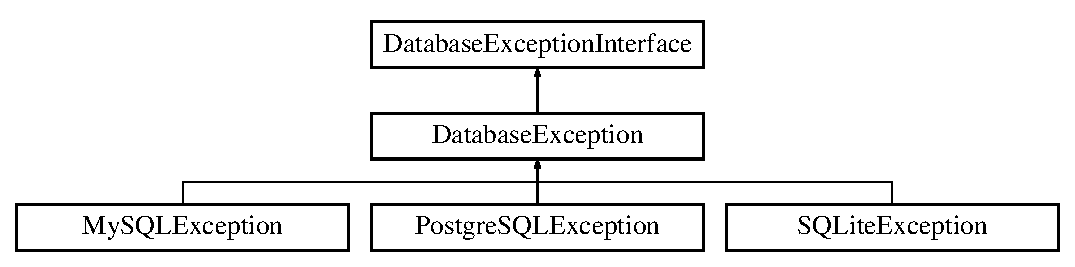
\includegraphics[height=3.000000cm]{class_database_exception}
\end{center}
\end{figure}
\subsection*{Public Member Functions}
\begin{DoxyCompactItemize}
\item 
\hyperlink{class_database_exception_ad1f01ac86a6ae06c72165c3a7cb0424a}{\+\_\+\+\_\+construct} (\&\$caller, \$message=null, \$code=null, \&\$caught=null)
\item 
\& \hyperlink{class_database_exception_aedb1e2149e60e99bd62a64f5533c7903}{get\+Caller} ()
\item 
\hyperlink{class_database_exception_aaf4fb3a4978596f9e37fdbdd1e786082}{get\+Error\+Flag} ()
\end{DoxyCompactItemize}
\subsection*{Data Fields}
\begin{DoxyCompactItemize}
\item 
const \hyperlink{class_database_exception_a93f610f377641d6a80dc3ba2c0d282cd}{E\+X\+C\+E\+P\+T\+I\+O\+N\+\_\+\+N\+O\+\_\+\+E\+R\+R\+O\+R} = 0
\item 
const \hyperlink{class_database_exception_ad70fde01b9fdf6cab7de36cb7f2329dd}{E\+X\+C\+E\+P\+T\+I\+O\+N\+\_\+\+T\+E\+S\+T} = 1
\item 
const \hyperlink{class_database_exception_a1531374c43d8490500ae0220d0b4a45a}{E\+X\+C\+E\+P\+T\+I\+O\+N\+\_\+\+G\+E\+N\+E\+R\+I\+C\+\_\+\+E\+R\+R\+O\+R} = 2
\item 
const \hyperlink{class_database_exception_aa329d5b77c2ad7a40e283926c6c6dc2e}{E\+X\+C\+E\+P\+T\+I\+O\+N\+\_\+\+U\+N\+C\+A\+U\+G\+H\+T\+\_\+\+E\+X\+C\+E\+P\+T\+I\+O\+N} = 3
\item 
const \hyperlink{class_database_exception_a9214bdd72834d71914a74f0a27db4a1e}{E\+X\+C\+E\+P\+T\+I\+O\+N\+\_\+\+I\+N\+V\+A\+L\+I\+D\+\_\+\+E\+X\+C\+E\+P\+T\+I\+O\+N} = 4
\item 
const \hyperlink{class_database_exception_af16d7ab9f9f71d7ac961a10a2eb9ec65}{E\+X\+C\+E\+P\+T\+I\+O\+N\+\_\+\+G\+E\+N\+E\+R\+I\+C\+\_\+\+I\+N\+P\+U\+T\+\_\+\+E\+R\+R\+O\+R} = 1000
\item 
const \hyperlink{class_database_exception_ab85a8b8e512fdab1e0f3a0ca8be9aaa0}{E\+X\+C\+E\+P\+T\+I\+O\+N\+\_\+\+I\+N\+P\+U\+T\+\_\+\+I\+N\+V\+A\+L\+I\+D\+\_\+\+T\+Y\+P\+E} = 1001
\item 
const \hyperlink{class_database_exception_aecec182787a871e4c5c0a2f4110f9920}{E\+X\+C\+E\+P\+T\+I\+O\+N\+\_\+\+I\+N\+P\+U\+T\+\_\+\+N\+O\+T\+\_\+\+V\+A\+L\+I\+D} = 1002
\item 
const \hyperlink{class_database_exception_a5e32a0f3e8b89279262617564b4c39a2}{E\+X\+C\+E\+P\+T\+I\+O\+N\+\_\+\+I\+N\+V\+A\+L\+I\+D\+\_\+\+D\+A\+T\+A\+B\+A\+S\+E\+\_\+\+T\+Y\+P\+E} = 1003
\item 
const \hyperlink{class_database_exception_a95a9d1ff5c1d06fff7293ea4b61af959}{E\+X\+C\+E\+P\+T\+I\+O\+N\+\_\+\+M\+I\+S\+S\+I\+N\+G\+\_\+\+R\+E\+Q\+U\+I\+R\+E\+D\+\_\+\+A\+R\+G\+U\+M\+E\+N\+T} = 1004
\item 
const \hyperlink{class_database_exception_acb77d344642fcd23d3007350580df264}{E\+X\+C\+E\+P\+T\+I\+O\+N\+\_\+\+M\+I\+S\+S\+I\+N\+G\+\_\+\+D\+E\+F\+I\+N\+I\+T\+I\+O\+N} = 1005
\item 
const \hyperlink{class_database_exception_a86c756dcdcdc0d6a13363e420b4b1ed6}{E\+X\+C\+E\+P\+T\+I\+O\+N\+\_\+\+I\+N\+P\+U\+T\+\_\+\+A\+R\+R\+A\+Y\+\_\+\+T\+O\+O\+\_\+\+D\+E\+E\+P} = 1006
\item 
const \hyperlink{class_database_exception_ab8d6e239e0336ea8b8e1203f6c38f3c7}{E\+X\+C\+E\+P\+T\+I\+O\+N\+\_\+\+I\+N\+P\+U\+T\+\_\+\+A\+R\+R\+A\+Y\+\_\+\+T\+O\+O\+\_\+\+S\+H\+A\+L\+L\+O\+W} = 1007
\item 
const \hyperlink{class_database_exception_a54384c002df87b714c8cd0d27db21f85}{E\+X\+C\+E\+P\+T\+I\+O\+N\+\_\+\+G\+E\+N\+E\+R\+I\+C\+\_\+\+D\+A\+T\+A\+B\+A\+S\+E\+\_\+\+E\+R\+R\+O\+R} = 2000
\item 
const \hyperlink{class_database_exception_a8c1f734137128a0b3a7ab767e583e7ad}{E\+X\+C\+E\+P\+T\+I\+O\+N\+\_\+\+T\+A\+B\+L\+E\+\_\+\+D\+O\+E\+S\+\_\+\+N\+O\+T\+\_\+\+E\+X\+I\+S\+T} = 2001
\item 
const \hyperlink{class_database_exception_ae8c6c4d6c53676f4dfc17c3acbc4e86a}{E\+X\+C\+E\+P\+T\+I\+O\+N\+\_\+\+D\+B\+\_\+\+I\+T\+E\+M\+\_\+\+C\+A\+N\+N\+O\+T\+\_\+\+B\+E\+\_\+\+C\+R\+E\+A\+T\+E\+D} = 2002
\item 
const \hyperlink{class_database_exception_a0d11e2b4e48912224166b8733bf7cee8}{E\+X\+C\+E\+P\+T\+I\+O\+N\+\_\+\+D\+B\+\_\+\+I\+T\+E\+M\+\_\+\+C\+A\+N\+N\+O\+T\+\_\+\+B\+E\+\_\+\+D\+R\+O\+P\+P\+E\+D} = 2003
\item 
const \hyperlink{class_database_exception_a3adbce979bbf4f1f99b59bb62555307f}{E\+X\+C\+E\+P\+T\+I\+O\+N\+\_\+\+D\+B\+\_\+\+I\+T\+E\+M\+\_\+\+A\+L\+R\+E\+A\+D\+Y\+\_\+\+E\+X\+I\+S\+T\+S} = 2004
\item 
const \hyperlink{class_database_exception_a051a953b3dbf5c69685ae0905d68a2cb}{E\+X\+C\+E\+P\+T\+I\+O\+N\+\_\+\+D\+B\+\_\+\+I\+T\+E\+M\+\_\+\+D\+O\+E\+S\+\_\+\+N\+O\+T\+\_\+\+E\+X\+I\+S\+T} = 2005
\item 
const \hyperlink{class_database_exception_aafe8d0c8826d17ec598136f35e381524}{E\+X\+C\+E\+P\+T\+I\+O\+N\+\_\+\+D\+B\+\_\+\+O\+P\+E\+R\+A\+T\+I\+O\+N\+\_\+\+L\+O\+C\+K\+E\+D} = 2005
\item 
const \hyperlink{class_database_exception_a314fb08476b7cab00496a16cfa30708f}{E\+X\+C\+E\+P\+T\+I\+O\+N\+\_\+\+D\+B\+\_\+\+O\+P\+E\+R\+A\+T\+I\+O\+N\+\_\+\+R\+E\+A\+D\+\_\+\+O\+N\+L\+Y} = 2006
\item 
const \hyperlink{class_database_exception_af4c8c1347d3322d171c556f518fb75a6}{E\+X\+C\+E\+P\+T\+I\+O\+N\+\_\+\+D\+B\+\_\+\+C\+A\+N\+N\+O\+T\+\_\+\+R\+E\+A\+D\+\_\+\+R\+E\+C\+O\+R\+D} = 2007
\item 
const \hyperlink{class_database_exception_a078837d5b35b669c158aa3cc2c0e2a9f}{E\+X\+C\+E\+P\+T\+I\+O\+N\+\_\+\+D\+B\+\_\+\+C\+A\+N\+N\+O\+T\+\_\+\+G\+E\+T\+\_\+\+S\+T\+A\+T\+U\+S} = 2008
\item 
const \hyperlink{class_database_exception_aa49625b4d6d958dd9dff0969725eec8b}{E\+X\+C\+E\+P\+T\+I\+O\+N\+\_\+\+D\+B\+\_\+\+R\+E\+C\+O\+R\+D\+\_\+\+I\+N\+C\+O\+N\+S\+I\+S\+T\+E\+N\+C\+Y} = 2009
\item 
const \hyperlink{class_database_exception_ac2b0baa16c6c435065699e0606272706}{E\+X\+C\+E\+P\+T\+I\+O\+N\+\_\+\+G\+E\+N\+E\+R\+I\+C\+\_\+\+S\+Y\+S\+T\+E\+M\+\_\+\+E\+R\+R\+O\+R} = 3000
\item 
const \hyperlink{class_database_exception_a460f308cd80a87c48d51ac54e61b37bc}{E\+X\+C\+E\+P\+T\+I\+O\+N\+\_\+\+F\+S\+\_\+\+C\+A\+N\+N\+O\+T\+\_\+\+O\+P\+E\+N\+\_\+\+F\+I\+L\+E} = 3001
\item 
const \hyperlink{class_database_exception_a4cde73367b61f571c353362002618265}{E\+X\+C\+E\+P\+T\+I\+O\+N\+\_\+\+F\+S\+\_\+\+C\+A\+N\+N\+O\+T\+\_\+\+A\+C\+C\+E\+S\+S\+\_\+\+D\+I\+R} = 3002
\item 
const \hyperlink{class_database_exception_ada70b9523f11c2115e75b0c1298b7b95}{E\+X\+C\+E\+P\+T\+I\+O\+N\+\_\+\+F\+S\+\_\+\+C\+A\+N\+N\+O\+T\+\_\+\+C\+R\+E\+A\+T\+E\+\_\+\+F\+I\+L\+E} = 3003
\item 
const \hyperlink{class_database_exception_ab8908292d329eb19e5e2a01e65efec4a}{E\+X\+C\+E\+P\+T\+I\+O\+N\+\_\+\+F\+S\+\_\+\+C\+A\+N\+N\+O\+T\+\_\+\+D\+E\+L\+E\+T\+E\+\_\+\+F\+I\+L\+E} = 3004
\item 
const \hyperlink{class_database_exception_aba74a043f93aff28bf7d913d64504889}{E\+X\+C\+E\+P\+T\+I\+O\+N\+\_\+\+F\+S\+\_\+\+F\+I\+L\+E\+\_\+\+N\+O\+T\+\_\+\+F\+O\+U\+N\+D} = 3005
\item 
const \hyperlink{class_database_exception_a1d7160b183812594679877046c3fd62a}{E\+X\+C\+E\+P\+T\+I\+O\+N\+\_\+\+F\+S\+\_\+\+O\+U\+T\+\_\+\+O\+F\+\_\+\+S\+P\+A\+C\+E} = 3006
\item 
const \hyperlink{class_database_exception_aa1ed10447564eb986514790822a1516c}{E\+X\+C\+E\+P\+T\+I\+O\+N\+\_\+\+F\+S\+\_\+\+P\+E\+R\+M\+I\+S\+S\+I\+O\+N\+S\+\_\+\+E\+R\+R\+O\+R} = 3007
\item 
const \hyperlink{class_database_exception_a40d50055804a9019ed22faec53b5f7ca}{E\+X\+C\+E\+P\+T\+I\+O\+N\+\_\+\+F\+S\+\_\+\+C\+A\+N\+N\+O\+T\+\_\+\+G\+E\+T\+\_\+\+C\+W\+D} = 3008
\item 
const \hyperlink{class_database_exception_ac5a6423e46a25c86b58d3f6fb5b55c9d}{E\+X\+C\+E\+P\+T\+I\+O\+N\+\_\+\+F\+S\+\_\+\+C\+A\+N\+N\+O\+T\+\_\+\+L\+O\+C\+K\+\_\+\+F\+I\+L\+E} = 3009
\item 
const \hyperlink{class_database_exception_afb0b7d842c8de8754481a086fbaea08d}{E\+X\+C\+E\+P\+T\+I\+O\+N\+\_\+\+F\+S\+\_\+\+C\+A\+N\+N\+O\+T\+\_\+\+C\+H\+A\+N\+G\+E\+\_\+\+D\+I\+R} = 3010
\item 
const \hyperlink{class_database_exception_ab186397805d52a7001f613304dee257a}{E\+X\+C\+E\+P\+T\+I\+O\+N\+\_\+\+G\+E\+N\+E\+R\+I\+C\+\_\+\+N\+E\+T\+W\+O\+R\+K\+\_\+\+E\+R\+R\+O\+R} = 4000
\item 
const \hyperlink{class_database_exception_a53179a0bedcb9a50567afed3ae66baaa}{E\+X\+C\+E\+P\+T\+I\+O\+N\+\_\+\+N\+E\+T\+\_\+\+T\+I\+M\+E\+O\+U\+T} = 4001
\item 
const \hyperlink{class_database_exception_aaa5b45b9fc8dc9eaf84c2b846fbb9cc1}{E\+X\+C\+E\+P\+T\+I\+O\+N\+\_\+\+N\+E\+T\+\_\+\+R\+E\+S\+E\+T\+\_\+\+B\+Y\+\_\+\+P\+E\+E\+R} = 4002
\item 
const \hyperlink{class_database_exception_abbef5bf22fd6bb11a46837ba48e8bf00}{E\+X\+C\+E\+P\+T\+I\+O\+N\+\_\+\+N\+E\+T\+\_\+\+C\+O\+N\+N\+E\+C\+T\+I\+O\+N\+\_\+\+R\+E\+F\+U\+S\+E\+D} = 4003
\end{DoxyCompactItemize}
\subsection*{Protected Member Functions}
\begin{DoxyCompactItemize}
\item 
\hyperlink{class_database_exception_a37357ff7fe8d1c1ea764fa1465637543}{get\+Constants} ()
\end{DoxyCompactItemize}
\subsection*{Protected Attributes}
\begin{DoxyCompactItemize}
\item 
\hyperlink{class_database_exception_a0b21046130eb880a92ca750675597c75}{\$caller}
\item 
\hyperlink{class_database_exception_a461278c71fc5038037fac5e2f5e1c6af}{\$caught}
\end{DoxyCompactItemize}


\subsection{Detailed Description}


Definition at line 3 of file Database\+Exception.\+php.



\subsection{Constructor \& Destructor Documentation}
\hypertarget{class_database_exception_ad1f01ac86a6ae06c72165c3a7cb0424a}{}\index{Database\+Exception@{Database\+Exception}!\+\_\+\+\_\+construct@{\+\_\+\+\_\+construct}}
\index{\+\_\+\+\_\+construct@{\+\_\+\+\_\+construct}!Database\+Exception@{Database\+Exception}}
\subsubsection[{\+\_\+\+\_\+construct}]{\setlength{\rightskip}{0pt plus 5cm}\+\_\+\+\_\+construct (
\begin{DoxyParamCaption}
\item[{\&}]{\$caller, }
\item[{}]{\$message = {\ttfamily null}, }
\item[{}]{\$code = {\ttfamily null}, }
\item[{\&}]{\$caught = {\ttfamily null}}
\end{DoxyParamCaption}
)}\label{class_database_exception_ad1f01ac86a6ae06c72165c3a7cb0424a}
Constructor Method


\begin{DoxyParams}{Parameters}
{\em \$parent} & (required) -\/ \\
\hline
\end{DoxyParams}


Implements \hyperlink{interface_database_exception_interface_ad1f01ac86a6ae06c72165c3a7cb0424a}{Database\+Exception\+Interface}.



Definition at line 62 of file Database\+Exception.\+php.



\subsection{Member Function Documentation}
\hypertarget{class_database_exception_aedb1e2149e60e99bd62a64f5533c7903}{}\index{Database\+Exception@{Database\+Exception}!get\+Caller@{get\+Caller}}
\index{get\+Caller@{get\+Caller}!Database\+Exception@{Database\+Exception}}
\subsubsection[{get\+Caller}]{\setlength{\rightskip}{0pt plus 5cm}\& get\+Caller (
\begin{DoxyParamCaption}
{}
\end{DoxyParamCaption}
)}\label{class_database_exception_aedb1e2149e60e99bd62a64f5533c7903}


Implements \hyperlink{interface_database_exception_interface_aedb1e2149e60e99bd62a64f5533c7903}{Database\+Exception\+Interface}.



Definition at line 86 of file Database\+Exception.\+php.

\hypertarget{class_database_exception_a37357ff7fe8d1c1ea764fa1465637543}{}\index{Database\+Exception@{Database\+Exception}!get\+Constants@{get\+Constants}}
\index{get\+Constants@{get\+Constants}!Database\+Exception@{Database\+Exception}}
\subsubsection[{get\+Constants}]{\setlength{\rightskip}{0pt plus 5cm}get\+Constants (
\begin{DoxyParamCaption}
{}
\end{DoxyParamCaption}
)\hspace{0.3cm}{\ttfamily [final]}, {\ttfamily [protected]}}\label{class_database_exception_a37357ff7fe8d1c1ea764fa1465637543}
Database\+Exception-\/$>$\hyperlink{class_database_exception_a37357ff7fe8d1c1ea764fa1465637543}{get\+Constants()} protected Method

gets an array of constants for the \hyperlink{class_database_exception}{Database\+Exception} object

\begin{DoxyReturn}{Returns}
array -\/ Array of constants as constant\+Name =$>$ constant\+Value 
\end{DoxyReturn}


Implements \hyperlink{interface_database_exception_interface_a37357ff7fe8d1c1ea764fa1465637543}{Database\+Exception\+Interface}.



Definition at line 99 of file Database\+Exception.\+php.

\hypertarget{class_database_exception_aaf4fb3a4978596f9e37fdbdd1e786082}{}\index{Database\+Exception@{Database\+Exception}!get\+Error\+Flag@{get\+Error\+Flag}}
\index{get\+Error\+Flag@{get\+Error\+Flag}!Database\+Exception@{Database\+Exception}}
\subsubsection[{get\+Error\+Flag}]{\setlength{\rightskip}{0pt plus 5cm}get\+Error\+Flag (
\begin{DoxyParamCaption}
{}
\end{DoxyParamCaption}
)}\label{class_database_exception_aaf4fb3a4978596f9e37fdbdd1e786082}
Database\+Exception-\/$>$\hyperlink{class_database_exception_aaf4fb3a4978596f9e37fdbdd1e786082}{get\+Error\+Flag()} Method

gets the flag (constant) name of the exception\textquotesingle{}s error type

\begin{DoxyReturn}{Returns}
string -\/ Name of flag of the exception\textquotesingle{}s error type 
\end{DoxyReturn}


Implements \hyperlink{interface_database_exception_interface_aaf4fb3a4978596f9e37fdbdd1e786082}{Database\+Exception\+Interface}.



Definition at line 113 of file Database\+Exception.\+php.



\subsection{Field Documentation}
\hypertarget{class_database_exception_a0b21046130eb880a92ca750675597c75}{}\index{Database\+Exception@{Database\+Exception}!\$caller@{\$caller}}
\index{\$caller@{\$caller}!Database\+Exception@{Database\+Exception}}
\subsubsection[{\$caller}]{\setlength{\rightskip}{0pt plus 5cm}\$caller\hspace{0.3cm}{\ttfamily [protected]}}\label{class_database_exception_a0b21046130eb880a92ca750675597c75}


Definition at line 5 of file Database\+Exception.\+php.

\hypertarget{class_database_exception_a461278c71fc5038037fac5e2f5e1c6af}{}\index{Database\+Exception@{Database\+Exception}!\$caught@{\$caught}}
\index{\$caught@{\$caught}!Database\+Exception@{Database\+Exception}}
\subsubsection[{\$caught}]{\setlength{\rightskip}{0pt plus 5cm}\$caught\hspace{0.3cm}{\ttfamily [protected]}}\label{class_database_exception_a461278c71fc5038037fac5e2f5e1c6af}


Definition at line 6 of file Database\+Exception.\+php.

\hypertarget{class_database_exception_a078837d5b35b669c158aa3cc2c0e2a9f}{}\index{Database\+Exception@{Database\+Exception}!E\+X\+C\+E\+P\+T\+I\+O\+N\+\_\+\+D\+B\+\_\+\+C\+A\+N\+N\+O\+T\+\_\+\+G\+E\+T\+\_\+\+S\+T\+A\+T\+U\+S@{E\+X\+C\+E\+P\+T\+I\+O\+N\+\_\+\+D\+B\+\_\+\+C\+A\+N\+N\+O\+T\+\_\+\+G\+E\+T\+\_\+\+S\+T\+A\+T\+U\+S}}
\index{E\+X\+C\+E\+P\+T\+I\+O\+N\+\_\+\+D\+B\+\_\+\+C\+A\+N\+N\+O\+T\+\_\+\+G\+E\+T\+\_\+\+S\+T\+A\+T\+U\+S@{E\+X\+C\+E\+P\+T\+I\+O\+N\+\_\+\+D\+B\+\_\+\+C\+A\+N\+N\+O\+T\+\_\+\+G\+E\+T\+\_\+\+S\+T\+A\+T\+U\+S}!Database\+Exception@{Database\+Exception}}
\subsubsection[{E\+X\+C\+E\+P\+T\+I\+O\+N\+\_\+\+D\+B\+\_\+\+C\+A\+N\+N\+O\+T\+\_\+\+G\+E\+T\+\_\+\+S\+T\+A\+T\+U\+S}]{\setlength{\rightskip}{0pt plus 5cm}const E\+X\+C\+E\+P\+T\+I\+O\+N\+\_\+\+D\+B\+\_\+\+C\+A\+N\+N\+O\+T\+\_\+\+G\+E\+T\+\_\+\+S\+T\+A\+T\+U\+S = 2008}\label{class_database_exception_a078837d5b35b669c158aa3cc2c0e2a9f}


Definition at line 35 of file Database\+Exception.\+php.

\hypertarget{class_database_exception_af4c8c1347d3322d171c556f518fb75a6}{}\index{Database\+Exception@{Database\+Exception}!E\+X\+C\+E\+P\+T\+I\+O\+N\+\_\+\+D\+B\+\_\+\+C\+A\+N\+N\+O\+T\+\_\+\+R\+E\+A\+D\+\_\+\+R\+E\+C\+O\+R\+D@{E\+X\+C\+E\+P\+T\+I\+O\+N\+\_\+\+D\+B\+\_\+\+C\+A\+N\+N\+O\+T\+\_\+\+R\+E\+A\+D\+\_\+\+R\+E\+C\+O\+R\+D}}
\index{E\+X\+C\+E\+P\+T\+I\+O\+N\+\_\+\+D\+B\+\_\+\+C\+A\+N\+N\+O\+T\+\_\+\+R\+E\+A\+D\+\_\+\+R\+E\+C\+O\+R\+D@{E\+X\+C\+E\+P\+T\+I\+O\+N\+\_\+\+D\+B\+\_\+\+C\+A\+N\+N\+O\+T\+\_\+\+R\+E\+A\+D\+\_\+\+R\+E\+C\+O\+R\+D}!Database\+Exception@{Database\+Exception}}
\subsubsection[{E\+X\+C\+E\+P\+T\+I\+O\+N\+\_\+\+D\+B\+\_\+\+C\+A\+N\+N\+O\+T\+\_\+\+R\+E\+A\+D\+\_\+\+R\+E\+C\+O\+R\+D}]{\setlength{\rightskip}{0pt plus 5cm}const E\+X\+C\+E\+P\+T\+I\+O\+N\+\_\+\+D\+B\+\_\+\+C\+A\+N\+N\+O\+T\+\_\+\+R\+E\+A\+D\+\_\+\+R\+E\+C\+O\+R\+D = 2007}\label{class_database_exception_af4c8c1347d3322d171c556f518fb75a6}


Definition at line 34 of file Database\+Exception.\+php.

\hypertarget{class_database_exception_a3adbce979bbf4f1f99b59bb62555307f}{}\index{Database\+Exception@{Database\+Exception}!E\+X\+C\+E\+P\+T\+I\+O\+N\+\_\+\+D\+B\+\_\+\+I\+T\+E\+M\+\_\+\+A\+L\+R\+E\+A\+D\+Y\+\_\+\+E\+X\+I\+S\+T\+S@{E\+X\+C\+E\+P\+T\+I\+O\+N\+\_\+\+D\+B\+\_\+\+I\+T\+E\+M\+\_\+\+A\+L\+R\+E\+A\+D\+Y\+\_\+\+E\+X\+I\+S\+T\+S}}
\index{E\+X\+C\+E\+P\+T\+I\+O\+N\+\_\+\+D\+B\+\_\+\+I\+T\+E\+M\+\_\+\+A\+L\+R\+E\+A\+D\+Y\+\_\+\+E\+X\+I\+S\+T\+S@{E\+X\+C\+E\+P\+T\+I\+O\+N\+\_\+\+D\+B\+\_\+\+I\+T\+E\+M\+\_\+\+A\+L\+R\+E\+A\+D\+Y\+\_\+\+E\+X\+I\+S\+T\+S}!Database\+Exception@{Database\+Exception}}
\subsubsection[{E\+X\+C\+E\+P\+T\+I\+O\+N\+\_\+\+D\+B\+\_\+\+I\+T\+E\+M\+\_\+\+A\+L\+R\+E\+A\+D\+Y\+\_\+\+E\+X\+I\+S\+T\+S}]{\setlength{\rightskip}{0pt plus 5cm}const E\+X\+C\+E\+P\+T\+I\+O\+N\+\_\+\+D\+B\+\_\+\+I\+T\+E\+M\+\_\+\+A\+L\+R\+E\+A\+D\+Y\+\_\+\+E\+X\+I\+S\+T\+S = 2004}\label{class_database_exception_a3adbce979bbf4f1f99b59bb62555307f}


Definition at line 30 of file Database\+Exception.\+php.

\hypertarget{class_database_exception_ae8c6c4d6c53676f4dfc17c3acbc4e86a}{}\index{Database\+Exception@{Database\+Exception}!E\+X\+C\+E\+P\+T\+I\+O\+N\+\_\+\+D\+B\+\_\+\+I\+T\+E\+M\+\_\+\+C\+A\+N\+N\+O\+T\+\_\+\+B\+E\+\_\+\+C\+R\+E\+A\+T\+E\+D@{E\+X\+C\+E\+P\+T\+I\+O\+N\+\_\+\+D\+B\+\_\+\+I\+T\+E\+M\+\_\+\+C\+A\+N\+N\+O\+T\+\_\+\+B\+E\+\_\+\+C\+R\+E\+A\+T\+E\+D}}
\index{E\+X\+C\+E\+P\+T\+I\+O\+N\+\_\+\+D\+B\+\_\+\+I\+T\+E\+M\+\_\+\+C\+A\+N\+N\+O\+T\+\_\+\+B\+E\+\_\+\+C\+R\+E\+A\+T\+E\+D@{E\+X\+C\+E\+P\+T\+I\+O\+N\+\_\+\+D\+B\+\_\+\+I\+T\+E\+M\+\_\+\+C\+A\+N\+N\+O\+T\+\_\+\+B\+E\+\_\+\+C\+R\+E\+A\+T\+E\+D}!Database\+Exception@{Database\+Exception}}
\subsubsection[{E\+X\+C\+E\+P\+T\+I\+O\+N\+\_\+\+D\+B\+\_\+\+I\+T\+E\+M\+\_\+\+C\+A\+N\+N\+O\+T\+\_\+\+B\+E\+\_\+\+C\+R\+E\+A\+T\+E\+D}]{\setlength{\rightskip}{0pt plus 5cm}const E\+X\+C\+E\+P\+T\+I\+O\+N\+\_\+\+D\+B\+\_\+\+I\+T\+E\+M\+\_\+\+C\+A\+N\+N\+O\+T\+\_\+\+B\+E\+\_\+\+C\+R\+E\+A\+T\+E\+D = 2002}\label{class_database_exception_ae8c6c4d6c53676f4dfc17c3acbc4e86a}


Definition at line 28 of file Database\+Exception.\+php.

\hypertarget{class_database_exception_a0d11e2b4e48912224166b8733bf7cee8}{}\index{Database\+Exception@{Database\+Exception}!E\+X\+C\+E\+P\+T\+I\+O\+N\+\_\+\+D\+B\+\_\+\+I\+T\+E\+M\+\_\+\+C\+A\+N\+N\+O\+T\+\_\+\+B\+E\+\_\+\+D\+R\+O\+P\+P\+E\+D@{E\+X\+C\+E\+P\+T\+I\+O\+N\+\_\+\+D\+B\+\_\+\+I\+T\+E\+M\+\_\+\+C\+A\+N\+N\+O\+T\+\_\+\+B\+E\+\_\+\+D\+R\+O\+P\+P\+E\+D}}
\index{E\+X\+C\+E\+P\+T\+I\+O\+N\+\_\+\+D\+B\+\_\+\+I\+T\+E\+M\+\_\+\+C\+A\+N\+N\+O\+T\+\_\+\+B\+E\+\_\+\+D\+R\+O\+P\+P\+E\+D@{E\+X\+C\+E\+P\+T\+I\+O\+N\+\_\+\+D\+B\+\_\+\+I\+T\+E\+M\+\_\+\+C\+A\+N\+N\+O\+T\+\_\+\+B\+E\+\_\+\+D\+R\+O\+P\+P\+E\+D}!Database\+Exception@{Database\+Exception}}
\subsubsection[{E\+X\+C\+E\+P\+T\+I\+O\+N\+\_\+\+D\+B\+\_\+\+I\+T\+E\+M\+\_\+\+C\+A\+N\+N\+O\+T\+\_\+\+B\+E\+\_\+\+D\+R\+O\+P\+P\+E\+D}]{\setlength{\rightskip}{0pt plus 5cm}const E\+X\+C\+E\+P\+T\+I\+O\+N\+\_\+\+D\+B\+\_\+\+I\+T\+E\+M\+\_\+\+C\+A\+N\+N\+O\+T\+\_\+\+B\+E\+\_\+\+D\+R\+O\+P\+P\+E\+D = 2003}\label{class_database_exception_a0d11e2b4e48912224166b8733bf7cee8}


Definition at line 29 of file Database\+Exception.\+php.

\hypertarget{class_database_exception_a051a953b3dbf5c69685ae0905d68a2cb}{}\index{Database\+Exception@{Database\+Exception}!E\+X\+C\+E\+P\+T\+I\+O\+N\+\_\+\+D\+B\+\_\+\+I\+T\+E\+M\+\_\+\+D\+O\+E\+S\+\_\+\+N\+O\+T\+\_\+\+E\+X\+I\+S\+T@{E\+X\+C\+E\+P\+T\+I\+O\+N\+\_\+\+D\+B\+\_\+\+I\+T\+E\+M\+\_\+\+D\+O\+E\+S\+\_\+\+N\+O\+T\+\_\+\+E\+X\+I\+S\+T}}
\index{E\+X\+C\+E\+P\+T\+I\+O\+N\+\_\+\+D\+B\+\_\+\+I\+T\+E\+M\+\_\+\+D\+O\+E\+S\+\_\+\+N\+O\+T\+\_\+\+E\+X\+I\+S\+T@{E\+X\+C\+E\+P\+T\+I\+O\+N\+\_\+\+D\+B\+\_\+\+I\+T\+E\+M\+\_\+\+D\+O\+E\+S\+\_\+\+N\+O\+T\+\_\+\+E\+X\+I\+S\+T}!Database\+Exception@{Database\+Exception}}
\subsubsection[{E\+X\+C\+E\+P\+T\+I\+O\+N\+\_\+\+D\+B\+\_\+\+I\+T\+E\+M\+\_\+\+D\+O\+E\+S\+\_\+\+N\+O\+T\+\_\+\+E\+X\+I\+S\+T}]{\setlength{\rightskip}{0pt plus 5cm}const E\+X\+C\+E\+P\+T\+I\+O\+N\+\_\+\+D\+B\+\_\+\+I\+T\+E\+M\+\_\+\+D\+O\+E\+S\+\_\+\+N\+O\+T\+\_\+\+E\+X\+I\+S\+T = 2005}\label{class_database_exception_a051a953b3dbf5c69685ae0905d68a2cb}


Definition at line 31 of file Database\+Exception.\+php.

\hypertarget{class_database_exception_aafe8d0c8826d17ec598136f35e381524}{}\index{Database\+Exception@{Database\+Exception}!E\+X\+C\+E\+P\+T\+I\+O\+N\+\_\+\+D\+B\+\_\+\+O\+P\+E\+R\+A\+T\+I\+O\+N\+\_\+\+L\+O\+C\+K\+E\+D@{E\+X\+C\+E\+P\+T\+I\+O\+N\+\_\+\+D\+B\+\_\+\+O\+P\+E\+R\+A\+T\+I\+O\+N\+\_\+\+L\+O\+C\+K\+E\+D}}
\index{E\+X\+C\+E\+P\+T\+I\+O\+N\+\_\+\+D\+B\+\_\+\+O\+P\+E\+R\+A\+T\+I\+O\+N\+\_\+\+L\+O\+C\+K\+E\+D@{E\+X\+C\+E\+P\+T\+I\+O\+N\+\_\+\+D\+B\+\_\+\+O\+P\+E\+R\+A\+T\+I\+O\+N\+\_\+\+L\+O\+C\+K\+E\+D}!Database\+Exception@{Database\+Exception}}
\subsubsection[{E\+X\+C\+E\+P\+T\+I\+O\+N\+\_\+\+D\+B\+\_\+\+O\+P\+E\+R\+A\+T\+I\+O\+N\+\_\+\+L\+O\+C\+K\+E\+D}]{\setlength{\rightskip}{0pt plus 5cm}const E\+X\+C\+E\+P\+T\+I\+O\+N\+\_\+\+D\+B\+\_\+\+O\+P\+E\+R\+A\+T\+I\+O\+N\+\_\+\+L\+O\+C\+K\+E\+D = 2005}\label{class_database_exception_aafe8d0c8826d17ec598136f35e381524}


Definition at line 32 of file Database\+Exception.\+php.

\hypertarget{class_database_exception_a314fb08476b7cab00496a16cfa30708f}{}\index{Database\+Exception@{Database\+Exception}!E\+X\+C\+E\+P\+T\+I\+O\+N\+\_\+\+D\+B\+\_\+\+O\+P\+E\+R\+A\+T\+I\+O\+N\+\_\+\+R\+E\+A\+D\+\_\+\+O\+N\+L\+Y@{E\+X\+C\+E\+P\+T\+I\+O\+N\+\_\+\+D\+B\+\_\+\+O\+P\+E\+R\+A\+T\+I\+O\+N\+\_\+\+R\+E\+A\+D\+\_\+\+O\+N\+L\+Y}}
\index{E\+X\+C\+E\+P\+T\+I\+O\+N\+\_\+\+D\+B\+\_\+\+O\+P\+E\+R\+A\+T\+I\+O\+N\+\_\+\+R\+E\+A\+D\+\_\+\+O\+N\+L\+Y@{E\+X\+C\+E\+P\+T\+I\+O\+N\+\_\+\+D\+B\+\_\+\+O\+P\+E\+R\+A\+T\+I\+O\+N\+\_\+\+R\+E\+A\+D\+\_\+\+O\+N\+L\+Y}!Database\+Exception@{Database\+Exception}}
\subsubsection[{E\+X\+C\+E\+P\+T\+I\+O\+N\+\_\+\+D\+B\+\_\+\+O\+P\+E\+R\+A\+T\+I\+O\+N\+\_\+\+R\+E\+A\+D\+\_\+\+O\+N\+L\+Y}]{\setlength{\rightskip}{0pt plus 5cm}const E\+X\+C\+E\+P\+T\+I\+O\+N\+\_\+\+D\+B\+\_\+\+O\+P\+E\+R\+A\+T\+I\+O\+N\+\_\+\+R\+E\+A\+D\+\_\+\+O\+N\+L\+Y = 2006}\label{class_database_exception_a314fb08476b7cab00496a16cfa30708f}


Definition at line 33 of file Database\+Exception.\+php.

\hypertarget{class_database_exception_aa49625b4d6d958dd9dff0969725eec8b}{}\index{Database\+Exception@{Database\+Exception}!E\+X\+C\+E\+P\+T\+I\+O\+N\+\_\+\+D\+B\+\_\+\+R\+E\+C\+O\+R\+D\+\_\+\+I\+N\+C\+O\+N\+S\+I\+S\+T\+E\+N\+C\+Y@{E\+X\+C\+E\+P\+T\+I\+O\+N\+\_\+\+D\+B\+\_\+\+R\+E\+C\+O\+R\+D\+\_\+\+I\+N\+C\+O\+N\+S\+I\+S\+T\+E\+N\+C\+Y}}
\index{E\+X\+C\+E\+P\+T\+I\+O\+N\+\_\+\+D\+B\+\_\+\+R\+E\+C\+O\+R\+D\+\_\+\+I\+N\+C\+O\+N\+S\+I\+S\+T\+E\+N\+C\+Y@{E\+X\+C\+E\+P\+T\+I\+O\+N\+\_\+\+D\+B\+\_\+\+R\+E\+C\+O\+R\+D\+\_\+\+I\+N\+C\+O\+N\+S\+I\+S\+T\+E\+N\+C\+Y}!Database\+Exception@{Database\+Exception}}
\subsubsection[{E\+X\+C\+E\+P\+T\+I\+O\+N\+\_\+\+D\+B\+\_\+\+R\+E\+C\+O\+R\+D\+\_\+\+I\+N\+C\+O\+N\+S\+I\+S\+T\+E\+N\+C\+Y}]{\setlength{\rightskip}{0pt plus 5cm}const E\+X\+C\+E\+P\+T\+I\+O\+N\+\_\+\+D\+B\+\_\+\+R\+E\+C\+O\+R\+D\+\_\+\+I\+N\+C\+O\+N\+S\+I\+S\+T\+E\+N\+C\+Y = 2009}\label{class_database_exception_aa49625b4d6d958dd9dff0969725eec8b}


Definition at line 36 of file Database\+Exception.\+php.

\hypertarget{class_database_exception_a4cde73367b61f571c353362002618265}{}\index{Database\+Exception@{Database\+Exception}!E\+X\+C\+E\+P\+T\+I\+O\+N\+\_\+\+F\+S\+\_\+\+C\+A\+N\+N\+O\+T\+\_\+\+A\+C\+C\+E\+S\+S\+\_\+\+D\+I\+R@{E\+X\+C\+E\+P\+T\+I\+O\+N\+\_\+\+F\+S\+\_\+\+C\+A\+N\+N\+O\+T\+\_\+\+A\+C\+C\+E\+S\+S\+\_\+\+D\+I\+R}}
\index{E\+X\+C\+E\+P\+T\+I\+O\+N\+\_\+\+F\+S\+\_\+\+C\+A\+N\+N\+O\+T\+\_\+\+A\+C\+C\+E\+S\+S\+\_\+\+D\+I\+R@{E\+X\+C\+E\+P\+T\+I\+O\+N\+\_\+\+F\+S\+\_\+\+C\+A\+N\+N\+O\+T\+\_\+\+A\+C\+C\+E\+S\+S\+\_\+\+D\+I\+R}!Database\+Exception@{Database\+Exception}}
\subsubsection[{E\+X\+C\+E\+P\+T\+I\+O\+N\+\_\+\+F\+S\+\_\+\+C\+A\+N\+N\+O\+T\+\_\+\+A\+C\+C\+E\+S\+S\+\_\+\+D\+I\+R}]{\setlength{\rightskip}{0pt plus 5cm}const E\+X\+C\+E\+P\+T\+I\+O\+N\+\_\+\+F\+S\+\_\+\+C\+A\+N\+N\+O\+T\+\_\+\+A\+C\+C\+E\+S\+S\+\_\+\+D\+I\+R = 3002}\label{class_database_exception_a4cde73367b61f571c353362002618265}


Definition at line 40 of file Database\+Exception.\+php.

\hypertarget{class_database_exception_afb0b7d842c8de8754481a086fbaea08d}{}\index{Database\+Exception@{Database\+Exception}!E\+X\+C\+E\+P\+T\+I\+O\+N\+\_\+\+F\+S\+\_\+\+C\+A\+N\+N\+O\+T\+\_\+\+C\+H\+A\+N\+G\+E\+\_\+\+D\+I\+R@{E\+X\+C\+E\+P\+T\+I\+O\+N\+\_\+\+F\+S\+\_\+\+C\+A\+N\+N\+O\+T\+\_\+\+C\+H\+A\+N\+G\+E\+\_\+\+D\+I\+R}}
\index{E\+X\+C\+E\+P\+T\+I\+O\+N\+\_\+\+F\+S\+\_\+\+C\+A\+N\+N\+O\+T\+\_\+\+C\+H\+A\+N\+G\+E\+\_\+\+D\+I\+R@{E\+X\+C\+E\+P\+T\+I\+O\+N\+\_\+\+F\+S\+\_\+\+C\+A\+N\+N\+O\+T\+\_\+\+C\+H\+A\+N\+G\+E\+\_\+\+D\+I\+R}!Database\+Exception@{Database\+Exception}}
\subsubsection[{E\+X\+C\+E\+P\+T\+I\+O\+N\+\_\+\+F\+S\+\_\+\+C\+A\+N\+N\+O\+T\+\_\+\+C\+H\+A\+N\+G\+E\+\_\+\+D\+I\+R}]{\setlength{\rightskip}{0pt plus 5cm}const E\+X\+C\+E\+P\+T\+I\+O\+N\+\_\+\+F\+S\+\_\+\+C\+A\+N\+N\+O\+T\+\_\+\+C\+H\+A\+N\+G\+E\+\_\+\+D\+I\+R = 3010}\label{class_database_exception_afb0b7d842c8de8754481a086fbaea08d}


Definition at line 48 of file Database\+Exception.\+php.

\hypertarget{class_database_exception_ada70b9523f11c2115e75b0c1298b7b95}{}\index{Database\+Exception@{Database\+Exception}!E\+X\+C\+E\+P\+T\+I\+O\+N\+\_\+\+F\+S\+\_\+\+C\+A\+N\+N\+O\+T\+\_\+\+C\+R\+E\+A\+T\+E\+\_\+\+F\+I\+L\+E@{E\+X\+C\+E\+P\+T\+I\+O\+N\+\_\+\+F\+S\+\_\+\+C\+A\+N\+N\+O\+T\+\_\+\+C\+R\+E\+A\+T\+E\+\_\+\+F\+I\+L\+E}}
\index{E\+X\+C\+E\+P\+T\+I\+O\+N\+\_\+\+F\+S\+\_\+\+C\+A\+N\+N\+O\+T\+\_\+\+C\+R\+E\+A\+T\+E\+\_\+\+F\+I\+L\+E@{E\+X\+C\+E\+P\+T\+I\+O\+N\+\_\+\+F\+S\+\_\+\+C\+A\+N\+N\+O\+T\+\_\+\+C\+R\+E\+A\+T\+E\+\_\+\+F\+I\+L\+E}!Database\+Exception@{Database\+Exception}}
\subsubsection[{E\+X\+C\+E\+P\+T\+I\+O\+N\+\_\+\+F\+S\+\_\+\+C\+A\+N\+N\+O\+T\+\_\+\+C\+R\+E\+A\+T\+E\+\_\+\+F\+I\+L\+E}]{\setlength{\rightskip}{0pt plus 5cm}const E\+X\+C\+E\+P\+T\+I\+O\+N\+\_\+\+F\+S\+\_\+\+C\+A\+N\+N\+O\+T\+\_\+\+C\+R\+E\+A\+T\+E\+\_\+\+F\+I\+L\+E = 3003}\label{class_database_exception_ada70b9523f11c2115e75b0c1298b7b95}


Definition at line 41 of file Database\+Exception.\+php.

\hypertarget{class_database_exception_ab8908292d329eb19e5e2a01e65efec4a}{}\index{Database\+Exception@{Database\+Exception}!E\+X\+C\+E\+P\+T\+I\+O\+N\+\_\+\+F\+S\+\_\+\+C\+A\+N\+N\+O\+T\+\_\+\+D\+E\+L\+E\+T\+E\+\_\+\+F\+I\+L\+E@{E\+X\+C\+E\+P\+T\+I\+O\+N\+\_\+\+F\+S\+\_\+\+C\+A\+N\+N\+O\+T\+\_\+\+D\+E\+L\+E\+T\+E\+\_\+\+F\+I\+L\+E}}
\index{E\+X\+C\+E\+P\+T\+I\+O\+N\+\_\+\+F\+S\+\_\+\+C\+A\+N\+N\+O\+T\+\_\+\+D\+E\+L\+E\+T\+E\+\_\+\+F\+I\+L\+E@{E\+X\+C\+E\+P\+T\+I\+O\+N\+\_\+\+F\+S\+\_\+\+C\+A\+N\+N\+O\+T\+\_\+\+D\+E\+L\+E\+T\+E\+\_\+\+F\+I\+L\+E}!Database\+Exception@{Database\+Exception}}
\subsubsection[{E\+X\+C\+E\+P\+T\+I\+O\+N\+\_\+\+F\+S\+\_\+\+C\+A\+N\+N\+O\+T\+\_\+\+D\+E\+L\+E\+T\+E\+\_\+\+F\+I\+L\+E}]{\setlength{\rightskip}{0pt plus 5cm}const E\+X\+C\+E\+P\+T\+I\+O\+N\+\_\+\+F\+S\+\_\+\+C\+A\+N\+N\+O\+T\+\_\+\+D\+E\+L\+E\+T\+E\+\_\+\+F\+I\+L\+E = 3004}\label{class_database_exception_ab8908292d329eb19e5e2a01e65efec4a}


Definition at line 42 of file Database\+Exception.\+php.

\hypertarget{class_database_exception_a40d50055804a9019ed22faec53b5f7ca}{}\index{Database\+Exception@{Database\+Exception}!E\+X\+C\+E\+P\+T\+I\+O\+N\+\_\+\+F\+S\+\_\+\+C\+A\+N\+N\+O\+T\+\_\+\+G\+E\+T\+\_\+\+C\+W\+D@{E\+X\+C\+E\+P\+T\+I\+O\+N\+\_\+\+F\+S\+\_\+\+C\+A\+N\+N\+O\+T\+\_\+\+G\+E\+T\+\_\+\+C\+W\+D}}
\index{E\+X\+C\+E\+P\+T\+I\+O\+N\+\_\+\+F\+S\+\_\+\+C\+A\+N\+N\+O\+T\+\_\+\+G\+E\+T\+\_\+\+C\+W\+D@{E\+X\+C\+E\+P\+T\+I\+O\+N\+\_\+\+F\+S\+\_\+\+C\+A\+N\+N\+O\+T\+\_\+\+G\+E\+T\+\_\+\+C\+W\+D}!Database\+Exception@{Database\+Exception}}
\subsubsection[{E\+X\+C\+E\+P\+T\+I\+O\+N\+\_\+\+F\+S\+\_\+\+C\+A\+N\+N\+O\+T\+\_\+\+G\+E\+T\+\_\+\+C\+W\+D}]{\setlength{\rightskip}{0pt plus 5cm}const E\+X\+C\+E\+P\+T\+I\+O\+N\+\_\+\+F\+S\+\_\+\+C\+A\+N\+N\+O\+T\+\_\+\+G\+E\+T\+\_\+\+C\+W\+D = 3008}\label{class_database_exception_a40d50055804a9019ed22faec53b5f7ca}


Definition at line 46 of file Database\+Exception.\+php.

\hypertarget{class_database_exception_ac5a6423e46a25c86b58d3f6fb5b55c9d}{}\index{Database\+Exception@{Database\+Exception}!E\+X\+C\+E\+P\+T\+I\+O\+N\+\_\+\+F\+S\+\_\+\+C\+A\+N\+N\+O\+T\+\_\+\+L\+O\+C\+K\+\_\+\+F\+I\+L\+E@{E\+X\+C\+E\+P\+T\+I\+O\+N\+\_\+\+F\+S\+\_\+\+C\+A\+N\+N\+O\+T\+\_\+\+L\+O\+C\+K\+\_\+\+F\+I\+L\+E}}
\index{E\+X\+C\+E\+P\+T\+I\+O\+N\+\_\+\+F\+S\+\_\+\+C\+A\+N\+N\+O\+T\+\_\+\+L\+O\+C\+K\+\_\+\+F\+I\+L\+E@{E\+X\+C\+E\+P\+T\+I\+O\+N\+\_\+\+F\+S\+\_\+\+C\+A\+N\+N\+O\+T\+\_\+\+L\+O\+C\+K\+\_\+\+F\+I\+L\+E}!Database\+Exception@{Database\+Exception}}
\subsubsection[{E\+X\+C\+E\+P\+T\+I\+O\+N\+\_\+\+F\+S\+\_\+\+C\+A\+N\+N\+O\+T\+\_\+\+L\+O\+C\+K\+\_\+\+F\+I\+L\+E}]{\setlength{\rightskip}{0pt plus 5cm}const E\+X\+C\+E\+P\+T\+I\+O\+N\+\_\+\+F\+S\+\_\+\+C\+A\+N\+N\+O\+T\+\_\+\+L\+O\+C\+K\+\_\+\+F\+I\+L\+E = 3009}\label{class_database_exception_ac5a6423e46a25c86b58d3f6fb5b55c9d}


Definition at line 47 of file Database\+Exception.\+php.

\hypertarget{class_database_exception_a460f308cd80a87c48d51ac54e61b37bc}{}\index{Database\+Exception@{Database\+Exception}!E\+X\+C\+E\+P\+T\+I\+O\+N\+\_\+\+F\+S\+\_\+\+C\+A\+N\+N\+O\+T\+\_\+\+O\+P\+E\+N\+\_\+\+F\+I\+L\+E@{E\+X\+C\+E\+P\+T\+I\+O\+N\+\_\+\+F\+S\+\_\+\+C\+A\+N\+N\+O\+T\+\_\+\+O\+P\+E\+N\+\_\+\+F\+I\+L\+E}}
\index{E\+X\+C\+E\+P\+T\+I\+O\+N\+\_\+\+F\+S\+\_\+\+C\+A\+N\+N\+O\+T\+\_\+\+O\+P\+E\+N\+\_\+\+F\+I\+L\+E@{E\+X\+C\+E\+P\+T\+I\+O\+N\+\_\+\+F\+S\+\_\+\+C\+A\+N\+N\+O\+T\+\_\+\+O\+P\+E\+N\+\_\+\+F\+I\+L\+E}!Database\+Exception@{Database\+Exception}}
\subsubsection[{E\+X\+C\+E\+P\+T\+I\+O\+N\+\_\+\+F\+S\+\_\+\+C\+A\+N\+N\+O\+T\+\_\+\+O\+P\+E\+N\+\_\+\+F\+I\+L\+E}]{\setlength{\rightskip}{0pt plus 5cm}const E\+X\+C\+E\+P\+T\+I\+O\+N\+\_\+\+F\+S\+\_\+\+C\+A\+N\+N\+O\+T\+\_\+\+O\+P\+E\+N\+\_\+\+F\+I\+L\+E = 3001}\label{class_database_exception_a460f308cd80a87c48d51ac54e61b37bc}


Definition at line 39 of file Database\+Exception.\+php.

\hypertarget{class_database_exception_aba74a043f93aff28bf7d913d64504889}{}\index{Database\+Exception@{Database\+Exception}!E\+X\+C\+E\+P\+T\+I\+O\+N\+\_\+\+F\+S\+\_\+\+F\+I\+L\+E\+\_\+\+N\+O\+T\+\_\+\+F\+O\+U\+N\+D@{E\+X\+C\+E\+P\+T\+I\+O\+N\+\_\+\+F\+S\+\_\+\+F\+I\+L\+E\+\_\+\+N\+O\+T\+\_\+\+F\+O\+U\+N\+D}}
\index{E\+X\+C\+E\+P\+T\+I\+O\+N\+\_\+\+F\+S\+\_\+\+F\+I\+L\+E\+\_\+\+N\+O\+T\+\_\+\+F\+O\+U\+N\+D@{E\+X\+C\+E\+P\+T\+I\+O\+N\+\_\+\+F\+S\+\_\+\+F\+I\+L\+E\+\_\+\+N\+O\+T\+\_\+\+F\+O\+U\+N\+D}!Database\+Exception@{Database\+Exception}}
\subsubsection[{E\+X\+C\+E\+P\+T\+I\+O\+N\+\_\+\+F\+S\+\_\+\+F\+I\+L\+E\+\_\+\+N\+O\+T\+\_\+\+F\+O\+U\+N\+D}]{\setlength{\rightskip}{0pt plus 5cm}const E\+X\+C\+E\+P\+T\+I\+O\+N\+\_\+\+F\+S\+\_\+\+F\+I\+L\+E\+\_\+\+N\+O\+T\+\_\+\+F\+O\+U\+N\+D = 3005}\label{class_database_exception_aba74a043f93aff28bf7d913d64504889}


Definition at line 43 of file Database\+Exception.\+php.

\hypertarget{class_database_exception_a1d7160b183812594679877046c3fd62a}{}\index{Database\+Exception@{Database\+Exception}!E\+X\+C\+E\+P\+T\+I\+O\+N\+\_\+\+F\+S\+\_\+\+O\+U\+T\+\_\+\+O\+F\+\_\+\+S\+P\+A\+C\+E@{E\+X\+C\+E\+P\+T\+I\+O\+N\+\_\+\+F\+S\+\_\+\+O\+U\+T\+\_\+\+O\+F\+\_\+\+S\+P\+A\+C\+E}}
\index{E\+X\+C\+E\+P\+T\+I\+O\+N\+\_\+\+F\+S\+\_\+\+O\+U\+T\+\_\+\+O\+F\+\_\+\+S\+P\+A\+C\+E@{E\+X\+C\+E\+P\+T\+I\+O\+N\+\_\+\+F\+S\+\_\+\+O\+U\+T\+\_\+\+O\+F\+\_\+\+S\+P\+A\+C\+E}!Database\+Exception@{Database\+Exception}}
\subsubsection[{E\+X\+C\+E\+P\+T\+I\+O\+N\+\_\+\+F\+S\+\_\+\+O\+U\+T\+\_\+\+O\+F\+\_\+\+S\+P\+A\+C\+E}]{\setlength{\rightskip}{0pt plus 5cm}const E\+X\+C\+E\+P\+T\+I\+O\+N\+\_\+\+F\+S\+\_\+\+O\+U\+T\+\_\+\+O\+F\+\_\+\+S\+P\+A\+C\+E = 3006}\label{class_database_exception_a1d7160b183812594679877046c3fd62a}


Definition at line 44 of file Database\+Exception.\+php.

\hypertarget{class_database_exception_aa1ed10447564eb986514790822a1516c}{}\index{Database\+Exception@{Database\+Exception}!E\+X\+C\+E\+P\+T\+I\+O\+N\+\_\+\+F\+S\+\_\+\+P\+E\+R\+M\+I\+S\+S\+I\+O\+N\+S\+\_\+\+E\+R\+R\+O\+R@{E\+X\+C\+E\+P\+T\+I\+O\+N\+\_\+\+F\+S\+\_\+\+P\+E\+R\+M\+I\+S\+S\+I\+O\+N\+S\+\_\+\+E\+R\+R\+O\+R}}
\index{E\+X\+C\+E\+P\+T\+I\+O\+N\+\_\+\+F\+S\+\_\+\+P\+E\+R\+M\+I\+S\+S\+I\+O\+N\+S\+\_\+\+E\+R\+R\+O\+R@{E\+X\+C\+E\+P\+T\+I\+O\+N\+\_\+\+F\+S\+\_\+\+P\+E\+R\+M\+I\+S\+S\+I\+O\+N\+S\+\_\+\+E\+R\+R\+O\+R}!Database\+Exception@{Database\+Exception}}
\subsubsection[{E\+X\+C\+E\+P\+T\+I\+O\+N\+\_\+\+F\+S\+\_\+\+P\+E\+R\+M\+I\+S\+S\+I\+O\+N\+S\+\_\+\+E\+R\+R\+O\+R}]{\setlength{\rightskip}{0pt plus 5cm}const E\+X\+C\+E\+P\+T\+I\+O\+N\+\_\+\+F\+S\+\_\+\+P\+E\+R\+M\+I\+S\+S\+I\+O\+N\+S\+\_\+\+E\+R\+R\+O\+R = 3007}\label{class_database_exception_aa1ed10447564eb986514790822a1516c}


Definition at line 45 of file Database\+Exception.\+php.

\hypertarget{class_database_exception_a54384c002df87b714c8cd0d27db21f85}{}\index{Database\+Exception@{Database\+Exception}!E\+X\+C\+E\+P\+T\+I\+O\+N\+\_\+\+G\+E\+N\+E\+R\+I\+C\+\_\+\+D\+A\+T\+A\+B\+A\+S\+E\+\_\+\+E\+R\+R\+O\+R@{E\+X\+C\+E\+P\+T\+I\+O\+N\+\_\+\+G\+E\+N\+E\+R\+I\+C\+\_\+\+D\+A\+T\+A\+B\+A\+S\+E\+\_\+\+E\+R\+R\+O\+R}}
\index{E\+X\+C\+E\+P\+T\+I\+O\+N\+\_\+\+G\+E\+N\+E\+R\+I\+C\+\_\+\+D\+A\+T\+A\+B\+A\+S\+E\+\_\+\+E\+R\+R\+O\+R@{E\+X\+C\+E\+P\+T\+I\+O\+N\+\_\+\+G\+E\+N\+E\+R\+I\+C\+\_\+\+D\+A\+T\+A\+B\+A\+S\+E\+\_\+\+E\+R\+R\+O\+R}!Database\+Exception@{Database\+Exception}}
\subsubsection[{E\+X\+C\+E\+P\+T\+I\+O\+N\+\_\+\+G\+E\+N\+E\+R\+I\+C\+\_\+\+D\+A\+T\+A\+B\+A\+S\+E\+\_\+\+E\+R\+R\+O\+R}]{\setlength{\rightskip}{0pt plus 5cm}const E\+X\+C\+E\+P\+T\+I\+O\+N\+\_\+\+G\+E\+N\+E\+R\+I\+C\+\_\+\+D\+A\+T\+A\+B\+A\+S\+E\+\_\+\+E\+R\+R\+O\+R = 2000}\label{class_database_exception_a54384c002df87b714c8cd0d27db21f85}


Definition at line 26 of file Database\+Exception.\+php.

\hypertarget{class_database_exception_a1531374c43d8490500ae0220d0b4a45a}{}\index{Database\+Exception@{Database\+Exception}!E\+X\+C\+E\+P\+T\+I\+O\+N\+\_\+\+G\+E\+N\+E\+R\+I\+C\+\_\+\+E\+R\+R\+O\+R@{E\+X\+C\+E\+P\+T\+I\+O\+N\+\_\+\+G\+E\+N\+E\+R\+I\+C\+\_\+\+E\+R\+R\+O\+R}}
\index{E\+X\+C\+E\+P\+T\+I\+O\+N\+\_\+\+G\+E\+N\+E\+R\+I\+C\+\_\+\+E\+R\+R\+O\+R@{E\+X\+C\+E\+P\+T\+I\+O\+N\+\_\+\+G\+E\+N\+E\+R\+I\+C\+\_\+\+E\+R\+R\+O\+R}!Database\+Exception@{Database\+Exception}}
\subsubsection[{E\+X\+C\+E\+P\+T\+I\+O\+N\+\_\+\+G\+E\+N\+E\+R\+I\+C\+\_\+\+E\+R\+R\+O\+R}]{\setlength{\rightskip}{0pt plus 5cm}const E\+X\+C\+E\+P\+T\+I\+O\+N\+\_\+\+G\+E\+N\+E\+R\+I\+C\+\_\+\+E\+R\+R\+O\+R = 2}\label{class_database_exception_a1531374c43d8490500ae0220d0b4a45a}


Definition at line 13 of file Database\+Exception.\+php.

\hypertarget{class_database_exception_af16d7ab9f9f71d7ac961a10a2eb9ec65}{}\index{Database\+Exception@{Database\+Exception}!E\+X\+C\+E\+P\+T\+I\+O\+N\+\_\+\+G\+E\+N\+E\+R\+I\+C\+\_\+\+I\+N\+P\+U\+T\+\_\+\+E\+R\+R\+O\+R@{E\+X\+C\+E\+P\+T\+I\+O\+N\+\_\+\+G\+E\+N\+E\+R\+I\+C\+\_\+\+I\+N\+P\+U\+T\+\_\+\+E\+R\+R\+O\+R}}
\index{E\+X\+C\+E\+P\+T\+I\+O\+N\+\_\+\+G\+E\+N\+E\+R\+I\+C\+\_\+\+I\+N\+P\+U\+T\+\_\+\+E\+R\+R\+O\+R@{E\+X\+C\+E\+P\+T\+I\+O\+N\+\_\+\+G\+E\+N\+E\+R\+I\+C\+\_\+\+I\+N\+P\+U\+T\+\_\+\+E\+R\+R\+O\+R}!Database\+Exception@{Database\+Exception}}
\subsubsection[{E\+X\+C\+E\+P\+T\+I\+O\+N\+\_\+\+G\+E\+N\+E\+R\+I\+C\+\_\+\+I\+N\+P\+U\+T\+\_\+\+E\+R\+R\+O\+R}]{\setlength{\rightskip}{0pt plus 5cm}const E\+X\+C\+E\+P\+T\+I\+O\+N\+\_\+\+G\+E\+N\+E\+R\+I\+C\+\_\+\+I\+N\+P\+U\+T\+\_\+\+E\+R\+R\+O\+R = 1000}\label{class_database_exception_af16d7ab9f9f71d7ac961a10a2eb9ec65}


Definition at line 17 of file Database\+Exception.\+php.

\hypertarget{class_database_exception_ab186397805d52a7001f613304dee257a}{}\index{Database\+Exception@{Database\+Exception}!E\+X\+C\+E\+P\+T\+I\+O\+N\+\_\+\+G\+E\+N\+E\+R\+I\+C\+\_\+\+N\+E\+T\+W\+O\+R\+K\+\_\+\+E\+R\+R\+O\+R@{E\+X\+C\+E\+P\+T\+I\+O\+N\+\_\+\+G\+E\+N\+E\+R\+I\+C\+\_\+\+N\+E\+T\+W\+O\+R\+K\+\_\+\+E\+R\+R\+O\+R}}
\index{E\+X\+C\+E\+P\+T\+I\+O\+N\+\_\+\+G\+E\+N\+E\+R\+I\+C\+\_\+\+N\+E\+T\+W\+O\+R\+K\+\_\+\+E\+R\+R\+O\+R@{E\+X\+C\+E\+P\+T\+I\+O\+N\+\_\+\+G\+E\+N\+E\+R\+I\+C\+\_\+\+N\+E\+T\+W\+O\+R\+K\+\_\+\+E\+R\+R\+O\+R}!Database\+Exception@{Database\+Exception}}
\subsubsection[{E\+X\+C\+E\+P\+T\+I\+O\+N\+\_\+\+G\+E\+N\+E\+R\+I\+C\+\_\+\+N\+E\+T\+W\+O\+R\+K\+\_\+\+E\+R\+R\+O\+R}]{\setlength{\rightskip}{0pt plus 5cm}const E\+X\+C\+E\+P\+T\+I\+O\+N\+\_\+\+G\+E\+N\+E\+R\+I\+C\+\_\+\+N\+E\+T\+W\+O\+R\+K\+\_\+\+E\+R\+R\+O\+R = 4000}\label{class_database_exception_ab186397805d52a7001f613304dee257a}


Definition at line 50 of file Database\+Exception.\+php.

\hypertarget{class_database_exception_ac2b0baa16c6c435065699e0606272706}{}\index{Database\+Exception@{Database\+Exception}!E\+X\+C\+E\+P\+T\+I\+O\+N\+\_\+\+G\+E\+N\+E\+R\+I\+C\+\_\+\+S\+Y\+S\+T\+E\+M\+\_\+\+E\+R\+R\+O\+R@{E\+X\+C\+E\+P\+T\+I\+O\+N\+\_\+\+G\+E\+N\+E\+R\+I\+C\+\_\+\+S\+Y\+S\+T\+E\+M\+\_\+\+E\+R\+R\+O\+R}}
\index{E\+X\+C\+E\+P\+T\+I\+O\+N\+\_\+\+G\+E\+N\+E\+R\+I\+C\+\_\+\+S\+Y\+S\+T\+E\+M\+\_\+\+E\+R\+R\+O\+R@{E\+X\+C\+E\+P\+T\+I\+O\+N\+\_\+\+G\+E\+N\+E\+R\+I\+C\+\_\+\+S\+Y\+S\+T\+E\+M\+\_\+\+E\+R\+R\+O\+R}!Database\+Exception@{Database\+Exception}}
\subsubsection[{E\+X\+C\+E\+P\+T\+I\+O\+N\+\_\+\+G\+E\+N\+E\+R\+I\+C\+\_\+\+S\+Y\+S\+T\+E\+M\+\_\+\+E\+R\+R\+O\+R}]{\setlength{\rightskip}{0pt plus 5cm}const E\+X\+C\+E\+P\+T\+I\+O\+N\+\_\+\+G\+E\+N\+E\+R\+I\+C\+\_\+\+S\+Y\+S\+T\+E\+M\+\_\+\+E\+R\+R\+O\+R = 3000}\label{class_database_exception_ac2b0baa16c6c435065699e0606272706}


Definition at line 38 of file Database\+Exception.\+php.

\hypertarget{class_database_exception_a86c756dcdcdc0d6a13363e420b4b1ed6}{}\index{Database\+Exception@{Database\+Exception}!E\+X\+C\+E\+P\+T\+I\+O\+N\+\_\+\+I\+N\+P\+U\+T\+\_\+\+A\+R\+R\+A\+Y\+\_\+\+T\+O\+O\+\_\+\+D\+E\+E\+P@{E\+X\+C\+E\+P\+T\+I\+O\+N\+\_\+\+I\+N\+P\+U\+T\+\_\+\+A\+R\+R\+A\+Y\+\_\+\+T\+O\+O\+\_\+\+D\+E\+E\+P}}
\index{E\+X\+C\+E\+P\+T\+I\+O\+N\+\_\+\+I\+N\+P\+U\+T\+\_\+\+A\+R\+R\+A\+Y\+\_\+\+T\+O\+O\+\_\+\+D\+E\+E\+P@{E\+X\+C\+E\+P\+T\+I\+O\+N\+\_\+\+I\+N\+P\+U\+T\+\_\+\+A\+R\+R\+A\+Y\+\_\+\+T\+O\+O\+\_\+\+D\+E\+E\+P}!Database\+Exception@{Database\+Exception}}
\subsubsection[{E\+X\+C\+E\+P\+T\+I\+O\+N\+\_\+\+I\+N\+P\+U\+T\+\_\+\+A\+R\+R\+A\+Y\+\_\+\+T\+O\+O\+\_\+\+D\+E\+E\+P}]{\setlength{\rightskip}{0pt plus 5cm}const E\+X\+C\+E\+P\+T\+I\+O\+N\+\_\+\+I\+N\+P\+U\+T\+\_\+\+A\+R\+R\+A\+Y\+\_\+\+T\+O\+O\+\_\+\+D\+E\+E\+P = 1006}\label{class_database_exception_a86c756dcdcdc0d6a13363e420b4b1ed6}


Definition at line 23 of file Database\+Exception.\+php.

\hypertarget{class_database_exception_ab8d6e239e0336ea8b8e1203f6c38f3c7}{}\index{Database\+Exception@{Database\+Exception}!E\+X\+C\+E\+P\+T\+I\+O\+N\+\_\+\+I\+N\+P\+U\+T\+\_\+\+A\+R\+R\+A\+Y\+\_\+\+T\+O\+O\+\_\+\+S\+H\+A\+L\+L\+O\+W@{E\+X\+C\+E\+P\+T\+I\+O\+N\+\_\+\+I\+N\+P\+U\+T\+\_\+\+A\+R\+R\+A\+Y\+\_\+\+T\+O\+O\+\_\+\+S\+H\+A\+L\+L\+O\+W}}
\index{E\+X\+C\+E\+P\+T\+I\+O\+N\+\_\+\+I\+N\+P\+U\+T\+\_\+\+A\+R\+R\+A\+Y\+\_\+\+T\+O\+O\+\_\+\+S\+H\+A\+L\+L\+O\+W@{E\+X\+C\+E\+P\+T\+I\+O\+N\+\_\+\+I\+N\+P\+U\+T\+\_\+\+A\+R\+R\+A\+Y\+\_\+\+T\+O\+O\+\_\+\+S\+H\+A\+L\+L\+O\+W}!Database\+Exception@{Database\+Exception}}
\subsubsection[{E\+X\+C\+E\+P\+T\+I\+O\+N\+\_\+\+I\+N\+P\+U\+T\+\_\+\+A\+R\+R\+A\+Y\+\_\+\+T\+O\+O\+\_\+\+S\+H\+A\+L\+L\+O\+W}]{\setlength{\rightskip}{0pt plus 5cm}const E\+X\+C\+E\+P\+T\+I\+O\+N\+\_\+\+I\+N\+P\+U\+T\+\_\+\+A\+R\+R\+A\+Y\+\_\+\+T\+O\+O\+\_\+\+S\+H\+A\+L\+L\+O\+W = 1007}\label{class_database_exception_ab8d6e239e0336ea8b8e1203f6c38f3c7}


Definition at line 24 of file Database\+Exception.\+php.

\hypertarget{class_database_exception_ab85a8b8e512fdab1e0f3a0ca8be9aaa0}{}\index{Database\+Exception@{Database\+Exception}!E\+X\+C\+E\+P\+T\+I\+O\+N\+\_\+\+I\+N\+P\+U\+T\+\_\+\+I\+N\+V\+A\+L\+I\+D\+\_\+\+T\+Y\+P\+E@{E\+X\+C\+E\+P\+T\+I\+O\+N\+\_\+\+I\+N\+P\+U\+T\+\_\+\+I\+N\+V\+A\+L\+I\+D\+\_\+\+T\+Y\+P\+E}}
\index{E\+X\+C\+E\+P\+T\+I\+O\+N\+\_\+\+I\+N\+P\+U\+T\+\_\+\+I\+N\+V\+A\+L\+I\+D\+\_\+\+T\+Y\+P\+E@{E\+X\+C\+E\+P\+T\+I\+O\+N\+\_\+\+I\+N\+P\+U\+T\+\_\+\+I\+N\+V\+A\+L\+I\+D\+\_\+\+T\+Y\+P\+E}!Database\+Exception@{Database\+Exception}}
\subsubsection[{E\+X\+C\+E\+P\+T\+I\+O\+N\+\_\+\+I\+N\+P\+U\+T\+\_\+\+I\+N\+V\+A\+L\+I\+D\+\_\+\+T\+Y\+P\+E}]{\setlength{\rightskip}{0pt plus 5cm}const E\+X\+C\+E\+P\+T\+I\+O\+N\+\_\+\+I\+N\+P\+U\+T\+\_\+\+I\+N\+V\+A\+L\+I\+D\+\_\+\+T\+Y\+P\+E = 1001}\label{class_database_exception_ab85a8b8e512fdab1e0f3a0ca8be9aaa0}


Definition at line 18 of file Database\+Exception.\+php.

\hypertarget{class_database_exception_aecec182787a871e4c5c0a2f4110f9920}{}\index{Database\+Exception@{Database\+Exception}!E\+X\+C\+E\+P\+T\+I\+O\+N\+\_\+\+I\+N\+P\+U\+T\+\_\+\+N\+O\+T\+\_\+\+V\+A\+L\+I\+D@{E\+X\+C\+E\+P\+T\+I\+O\+N\+\_\+\+I\+N\+P\+U\+T\+\_\+\+N\+O\+T\+\_\+\+V\+A\+L\+I\+D}}
\index{E\+X\+C\+E\+P\+T\+I\+O\+N\+\_\+\+I\+N\+P\+U\+T\+\_\+\+N\+O\+T\+\_\+\+V\+A\+L\+I\+D@{E\+X\+C\+E\+P\+T\+I\+O\+N\+\_\+\+I\+N\+P\+U\+T\+\_\+\+N\+O\+T\+\_\+\+V\+A\+L\+I\+D}!Database\+Exception@{Database\+Exception}}
\subsubsection[{E\+X\+C\+E\+P\+T\+I\+O\+N\+\_\+\+I\+N\+P\+U\+T\+\_\+\+N\+O\+T\+\_\+\+V\+A\+L\+I\+D}]{\setlength{\rightskip}{0pt plus 5cm}const E\+X\+C\+E\+P\+T\+I\+O\+N\+\_\+\+I\+N\+P\+U\+T\+\_\+\+N\+O\+T\+\_\+\+V\+A\+L\+I\+D = 1002}\label{class_database_exception_aecec182787a871e4c5c0a2f4110f9920}


Definition at line 19 of file Database\+Exception.\+php.

\hypertarget{class_database_exception_a5e32a0f3e8b89279262617564b4c39a2}{}\index{Database\+Exception@{Database\+Exception}!E\+X\+C\+E\+P\+T\+I\+O\+N\+\_\+\+I\+N\+V\+A\+L\+I\+D\+\_\+\+D\+A\+T\+A\+B\+A\+S\+E\+\_\+\+T\+Y\+P\+E@{E\+X\+C\+E\+P\+T\+I\+O\+N\+\_\+\+I\+N\+V\+A\+L\+I\+D\+\_\+\+D\+A\+T\+A\+B\+A\+S\+E\+\_\+\+T\+Y\+P\+E}}
\index{E\+X\+C\+E\+P\+T\+I\+O\+N\+\_\+\+I\+N\+V\+A\+L\+I\+D\+\_\+\+D\+A\+T\+A\+B\+A\+S\+E\+\_\+\+T\+Y\+P\+E@{E\+X\+C\+E\+P\+T\+I\+O\+N\+\_\+\+I\+N\+V\+A\+L\+I\+D\+\_\+\+D\+A\+T\+A\+B\+A\+S\+E\+\_\+\+T\+Y\+P\+E}!Database\+Exception@{Database\+Exception}}
\subsubsection[{E\+X\+C\+E\+P\+T\+I\+O\+N\+\_\+\+I\+N\+V\+A\+L\+I\+D\+\_\+\+D\+A\+T\+A\+B\+A\+S\+E\+\_\+\+T\+Y\+P\+E}]{\setlength{\rightskip}{0pt plus 5cm}const E\+X\+C\+E\+P\+T\+I\+O\+N\+\_\+\+I\+N\+V\+A\+L\+I\+D\+\_\+\+D\+A\+T\+A\+B\+A\+S\+E\+\_\+\+T\+Y\+P\+E = 1003}\label{class_database_exception_a5e32a0f3e8b89279262617564b4c39a2}


Definition at line 20 of file Database\+Exception.\+php.

\hypertarget{class_database_exception_a9214bdd72834d71914a74f0a27db4a1e}{}\index{Database\+Exception@{Database\+Exception}!E\+X\+C\+E\+P\+T\+I\+O\+N\+\_\+\+I\+N\+V\+A\+L\+I\+D\+\_\+\+E\+X\+C\+E\+P\+T\+I\+O\+N@{E\+X\+C\+E\+P\+T\+I\+O\+N\+\_\+\+I\+N\+V\+A\+L\+I\+D\+\_\+\+E\+X\+C\+E\+P\+T\+I\+O\+N}}
\index{E\+X\+C\+E\+P\+T\+I\+O\+N\+\_\+\+I\+N\+V\+A\+L\+I\+D\+\_\+\+E\+X\+C\+E\+P\+T\+I\+O\+N@{E\+X\+C\+E\+P\+T\+I\+O\+N\+\_\+\+I\+N\+V\+A\+L\+I\+D\+\_\+\+E\+X\+C\+E\+P\+T\+I\+O\+N}!Database\+Exception@{Database\+Exception}}
\subsubsection[{E\+X\+C\+E\+P\+T\+I\+O\+N\+\_\+\+I\+N\+V\+A\+L\+I\+D\+\_\+\+E\+X\+C\+E\+P\+T\+I\+O\+N}]{\setlength{\rightskip}{0pt plus 5cm}const E\+X\+C\+E\+P\+T\+I\+O\+N\+\_\+\+I\+N\+V\+A\+L\+I\+D\+\_\+\+E\+X\+C\+E\+P\+T\+I\+O\+N = 4}\label{class_database_exception_a9214bdd72834d71914a74f0a27db4a1e}


Definition at line 15 of file Database\+Exception.\+php.

\hypertarget{class_database_exception_acb77d344642fcd23d3007350580df264}{}\index{Database\+Exception@{Database\+Exception}!E\+X\+C\+E\+P\+T\+I\+O\+N\+\_\+\+M\+I\+S\+S\+I\+N\+G\+\_\+\+D\+E\+F\+I\+N\+I\+T\+I\+O\+N@{E\+X\+C\+E\+P\+T\+I\+O\+N\+\_\+\+M\+I\+S\+S\+I\+N\+G\+\_\+\+D\+E\+F\+I\+N\+I\+T\+I\+O\+N}}
\index{E\+X\+C\+E\+P\+T\+I\+O\+N\+\_\+\+M\+I\+S\+S\+I\+N\+G\+\_\+\+D\+E\+F\+I\+N\+I\+T\+I\+O\+N@{E\+X\+C\+E\+P\+T\+I\+O\+N\+\_\+\+M\+I\+S\+S\+I\+N\+G\+\_\+\+D\+E\+F\+I\+N\+I\+T\+I\+O\+N}!Database\+Exception@{Database\+Exception}}
\subsubsection[{E\+X\+C\+E\+P\+T\+I\+O\+N\+\_\+\+M\+I\+S\+S\+I\+N\+G\+\_\+\+D\+E\+F\+I\+N\+I\+T\+I\+O\+N}]{\setlength{\rightskip}{0pt plus 5cm}const E\+X\+C\+E\+P\+T\+I\+O\+N\+\_\+\+M\+I\+S\+S\+I\+N\+G\+\_\+\+D\+E\+F\+I\+N\+I\+T\+I\+O\+N = 1005}\label{class_database_exception_acb77d344642fcd23d3007350580df264}


Definition at line 22 of file Database\+Exception.\+php.

\hypertarget{class_database_exception_a95a9d1ff5c1d06fff7293ea4b61af959}{}\index{Database\+Exception@{Database\+Exception}!E\+X\+C\+E\+P\+T\+I\+O\+N\+\_\+\+M\+I\+S\+S\+I\+N\+G\+\_\+\+R\+E\+Q\+U\+I\+R\+E\+D\+\_\+\+A\+R\+G\+U\+M\+E\+N\+T@{E\+X\+C\+E\+P\+T\+I\+O\+N\+\_\+\+M\+I\+S\+S\+I\+N\+G\+\_\+\+R\+E\+Q\+U\+I\+R\+E\+D\+\_\+\+A\+R\+G\+U\+M\+E\+N\+T}}
\index{E\+X\+C\+E\+P\+T\+I\+O\+N\+\_\+\+M\+I\+S\+S\+I\+N\+G\+\_\+\+R\+E\+Q\+U\+I\+R\+E\+D\+\_\+\+A\+R\+G\+U\+M\+E\+N\+T@{E\+X\+C\+E\+P\+T\+I\+O\+N\+\_\+\+M\+I\+S\+S\+I\+N\+G\+\_\+\+R\+E\+Q\+U\+I\+R\+E\+D\+\_\+\+A\+R\+G\+U\+M\+E\+N\+T}!Database\+Exception@{Database\+Exception}}
\subsubsection[{E\+X\+C\+E\+P\+T\+I\+O\+N\+\_\+\+M\+I\+S\+S\+I\+N\+G\+\_\+\+R\+E\+Q\+U\+I\+R\+E\+D\+\_\+\+A\+R\+G\+U\+M\+E\+N\+T}]{\setlength{\rightskip}{0pt plus 5cm}const E\+X\+C\+E\+P\+T\+I\+O\+N\+\_\+\+M\+I\+S\+S\+I\+N\+G\+\_\+\+R\+E\+Q\+U\+I\+R\+E\+D\+\_\+\+A\+R\+G\+U\+M\+E\+N\+T = 1004}\label{class_database_exception_a95a9d1ff5c1d06fff7293ea4b61af959}


Definition at line 21 of file Database\+Exception.\+php.

\hypertarget{class_database_exception_abbef5bf22fd6bb11a46837ba48e8bf00}{}\index{Database\+Exception@{Database\+Exception}!E\+X\+C\+E\+P\+T\+I\+O\+N\+\_\+\+N\+E\+T\+\_\+\+C\+O\+N\+N\+E\+C\+T\+I\+O\+N\+\_\+\+R\+E\+F\+U\+S\+E\+D@{E\+X\+C\+E\+P\+T\+I\+O\+N\+\_\+\+N\+E\+T\+\_\+\+C\+O\+N\+N\+E\+C\+T\+I\+O\+N\+\_\+\+R\+E\+F\+U\+S\+E\+D}}
\index{E\+X\+C\+E\+P\+T\+I\+O\+N\+\_\+\+N\+E\+T\+\_\+\+C\+O\+N\+N\+E\+C\+T\+I\+O\+N\+\_\+\+R\+E\+F\+U\+S\+E\+D@{E\+X\+C\+E\+P\+T\+I\+O\+N\+\_\+\+N\+E\+T\+\_\+\+C\+O\+N\+N\+E\+C\+T\+I\+O\+N\+\_\+\+R\+E\+F\+U\+S\+E\+D}!Database\+Exception@{Database\+Exception}}
\subsubsection[{E\+X\+C\+E\+P\+T\+I\+O\+N\+\_\+\+N\+E\+T\+\_\+\+C\+O\+N\+N\+E\+C\+T\+I\+O\+N\+\_\+\+R\+E\+F\+U\+S\+E\+D}]{\setlength{\rightskip}{0pt plus 5cm}const E\+X\+C\+E\+P\+T\+I\+O\+N\+\_\+\+N\+E\+T\+\_\+\+C\+O\+N\+N\+E\+C\+T\+I\+O\+N\+\_\+\+R\+E\+F\+U\+S\+E\+D = 4003}\label{class_database_exception_abbef5bf22fd6bb11a46837ba48e8bf00}


Definition at line 53 of file Database\+Exception.\+php.

\hypertarget{class_database_exception_aaa5b45b9fc8dc9eaf84c2b846fbb9cc1}{}\index{Database\+Exception@{Database\+Exception}!E\+X\+C\+E\+P\+T\+I\+O\+N\+\_\+\+N\+E\+T\+\_\+\+R\+E\+S\+E\+T\+\_\+\+B\+Y\+\_\+\+P\+E\+E\+R@{E\+X\+C\+E\+P\+T\+I\+O\+N\+\_\+\+N\+E\+T\+\_\+\+R\+E\+S\+E\+T\+\_\+\+B\+Y\+\_\+\+P\+E\+E\+R}}
\index{E\+X\+C\+E\+P\+T\+I\+O\+N\+\_\+\+N\+E\+T\+\_\+\+R\+E\+S\+E\+T\+\_\+\+B\+Y\+\_\+\+P\+E\+E\+R@{E\+X\+C\+E\+P\+T\+I\+O\+N\+\_\+\+N\+E\+T\+\_\+\+R\+E\+S\+E\+T\+\_\+\+B\+Y\+\_\+\+P\+E\+E\+R}!Database\+Exception@{Database\+Exception}}
\subsubsection[{E\+X\+C\+E\+P\+T\+I\+O\+N\+\_\+\+N\+E\+T\+\_\+\+R\+E\+S\+E\+T\+\_\+\+B\+Y\+\_\+\+P\+E\+E\+R}]{\setlength{\rightskip}{0pt plus 5cm}const E\+X\+C\+E\+P\+T\+I\+O\+N\+\_\+\+N\+E\+T\+\_\+\+R\+E\+S\+E\+T\+\_\+\+B\+Y\+\_\+\+P\+E\+E\+R = 4002}\label{class_database_exception_aaa5b45b9fc8dc9eaf84c2b846fbb9cc1}


Definition at line 52 of file Database\+Exception.\+php.

\hypertarget{class_database_exception_a53179a0bedcb9a50567afed3ae66baaa}{}\index{Database\+Exception@{Database\+Exception}!E\+X\+C\+E\+P\+T\+I\+O\+N\+\_\+\+N\+E\+T\+\_\+\+T\+I\+M\+E\+O\+U\+T@{E\+X\+C\+E\+P\+T\+I\+O\+N\+\_\+\+N\+E\+T\+\_\+\+T\+I\+M\+E\+O\+U\+T}}
\index{E\+X\+C\+E\+P\+T\+I\+O\+N\+\_\+\+N\+E\+T\+\_\+\+T\+I\+M\+E\+O\+U\+T@{E\+X\+C\+E\+P\+T\+I\+O\+N\+\_\+\+N\+E\+T\+\_\+\+T\+I\+M\+E\+O\+U\+T}!Database\+Exception@{Database\+Exception}}
\subsubsection[{E\+X\+C\+E\+P\+T\+I\+O\+N\+\_\+\+N\+E\+T\+\_\+\+T\+I\+M\+E\+O\+U\+T}]{\setlength{\rightskip}{0pt plus 5cm}const E\+X\+C\+E\+P\+T\+I\+O\+N\+\_\+\+N\+E\+T\+\_\+\+T\+I\+M\+E\+O\+U\+T = 4001}\label{class_database_exception_a53179a0bedcb9a50567afed3ae66baaa}


Definition at line 51 of file Database\+Exception.\+php.

\hypertarget{class_database_exception_a93f610f377641d6a80dc3ba2c0d282cd}{}\index{Database\+Exception@{Database\+Exception}!E\+X\+C\+E\+P\+T\+I\+O\+N\+\_\+\+N\+O\+\_\+\+E\+R\+R\+O\+R@{E\+X\+C\+E\+P\+T\+I\+O\+N\+\_\+\+N\+O\+\_\+\+E\+R\+R\+O\+R}}
\index{E\+X\+C\+E\+P\+T\+I\+O\+N\+\_\+\+N\+O\+\_\+\+E\+R\+R\+O\+R@{E\+X\+C\+E\+P\+T\+I\+O\+N\+\_\+\+N\+O\+\_\+\+E\+R\+R\+O\+R}!Database\+Exception@{Database\+Exception}}
\subsubsection[{E\+X\+C\+E\+P\+T\+I\+O\+N\+\_\+\+N\+O\+\_\+\+E\+R\+R\+O\+R}]{\setlength{\rightskip}{0pt plus 5cm}const E\+X\+C\+E\+P\+T\+I\+O\+N\+\_\+\+N\+O\+\_\+\+E\+R\+R\+O\+R = 0}\label{class_database_exception_a93f610f377641d6a80dc3ba2c0d282cd}


Definition at line 11 of file Database\+Exception.\+php.

\hypertarget{class_database_exception_a8c1f734137128a0b3a7ab767e583e7ad}{}\index{Database\+Exception@{Database\+Exception}!E\+X\+C\+E\+P\+T\+I\+O\+N\+\_\+\+T\+A\+B\+L\+E\+\_\+\+D\+O\+E\+S\+\_\+\+N\+O\+T\+\_\+\+E\+X\+I\+S\+T@{E\+X\+C\+E\+P\+T\+I\+O\+N\+\_\+\+T\+A\+B\+L\+E\+\_\+\+D\+O\+E\+S\+\_\+\+N\+O\+T\+\_\+\+E\+X\+I\+S\+T}}
\index{E\+X\+C\+E\+P\+T\+I\+O\+N\+\_\+\+T\+A\+B\+L\+E\+\_\+\+D\+O\+E\+S\+\_\+\+N\+O\+T\+\_\+\+E\+X\+I\+S\+T@{E\+X\+C\+E\+P\+T\+I\+O\+N\+\_\+\+T\+A\+B\+L\+E\+\_\+\+D\+O\+E\+S\+\_\+\+N\+O\+T\+\_\+\+E\+X\+I\+S\+T}!Database\+Exception@{Database\+Exception}}
\subsubsection[{E\+X\+C\+E\+P\+T\+I\+O\+N\+\_\+\+T\+A\+B\+L\+E\+\_\+\+D\+O\+E\+S\+\_\+\+N\+O\+T\+\_\+\+E\+X\+I\+S\+T}]{\setlength{\rightskip}{0pt plus 5cm}const E\+X\+C\+E\+P\+T\+I\+O\+N\+\_\+\+T\+A\+B\+L\+E\+\_\+\+D\+O\+E\+S\+\_\+\+N\+O\+T\+\_\+\+E\+X\+I\+S\+T = 2001}\label{class_database_exception_a8c1f734137128a0b3a7ab767e583e7ad}


Definition at line 27 of file Database\+Exception.\+php.

\hypertarget{class_database_exception_ad70fde01b9fdf6cab7de36cb7f2329dd}{}\index{Database\+Exception@{Database\+Exception}!E\+X\+C\+E\+P\+T\+I\+O\+N\+\_\+\+T\+E\+S\+T@{E\+X\+C\+E\+P\+T\+I\+O\+N\+\_\+\+T\+E\+S\+T}}
\index{E\+X\+C\+E\+P\+T\+I\+O\+N\+\_\+\+T\+E\+S\+T@{E\+X\+C\+E\+P\+T\+I\+O\+N\+\_\+\+T\+E\+S\+T}!Database\+Exception@{Database\+Exception}}
\subsubsection[{E\+X\+C\+E\+P\+T\+I\+O\+N\+\_\+\+T\+E\+S\+T}]{\setlength{\rightskip}{0pt plus 5cm}const E\+X\+C\+E\+P\+T\+I\+O\+N\+\_\+\+T\+E\+S\+T = 1}\label{class_database_exception_ad70fde01b9fdf6cab7de36cb7f2329dd}


Definition at line 12 of file Database\+Exception.\+php.

\hypertarget{class_database_exception_aa329d5b77c2ad7a40e283926c6c6dc2e}{}\index{Database\+Exception@{Database\+Exception}!E\+X\+C\+E\+P\+T\+I\+O\+N\+\_\+\+U\+N\+C\+A\+U\+G\+H\+T\+\_\+\+E\+X\+C\+E\+P\+T\+I\+O\+N@{E\+X\+C\+E\+P\+T\+I\+O\+N\+\_\+\+U\+N\+C\+A\+U\+G\+H\+T\+\_\+\+E\+X\+C\+E\+P\+T\+I\+O\+N}}
\index{E\+X\+C\+E\+P\+T\+I\+O\+N\+\_\+\+U\+N\+C\+A\+U\+G\+H\+T\+\_\+\+E\+X\+C\+E\+P\+T\+I\+O\+N@{E\+X\+C\+E\+P\+T\+I\+O\+N\+\_\+\+U\+N\+C\+A\+U\+G\+H\+T\+\_\+\+E\+X\+C\+E\+P\+T\+I\+O\+N}!Database\+Exception@{Database\+Exception}}
\subsubsection[{E\+X\+C\+E\+P\+T\+I\+O\+N\+\_\+\+U\+N\+C\+A\+U\+G\+H\+T\+\_\+\+E\+X\+C\+E\+P\+T\+I\+O\+N}]{\setlength{\rightskip}{0pt plus 5cm}const E\+X\+C\+E\+P\+T\+I\+O\+N\+\_\+\+U\+N\+C\+A\+U\+G\+H\+T\+\_\+\+E\+X\+C\+E\+P\+T\+I\+O\+N = 3}\label{class_database_exception_aa329d5b77c2ad7a40e283926c6c6dc2e}


Definition at line 14 of file Database\+Exception.\+php.



The documentation for this class was generated from the following file\+:\begin{DoxyCompactItemize}
\item 
src/class/\hyperlink{_database_exception_8php}{Database\+Exception.\+php}\end{DoxyCompactItemize}

\hypertarget{interface_database_exception_interface}{}\section{Database\+Exception\+Interface Interface Reference}
\label{interface_database_exception_interface}\index{Database\+Exception\+Interface@{Database\+Exception\+Interface}}
Inheritance diagram for Database\+Exception\+Interface\+:\begin{figure}[H]
\begin{center}
\leavevmode
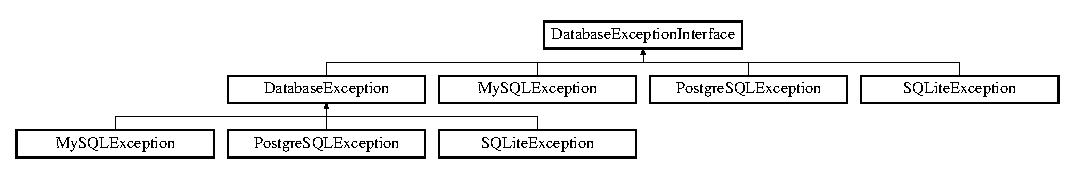
\includegraphics[height=1.573034cm]{interface_database_exception_interface}
\end{center}
\end{figure}
\subsection*{Public Member Functions}
\begin{DoxyCompactItemize}
\item 
\hyperlink{interface_database_exception_interface_ad1f01ac86a6ae06c72165c3a7cb0424a}{\+\_\+\+\_\+construct} (\&\$caller, \$message=null, \$code=null, \&\$caught=null)
\item 
\& \hyperlink{interface_database_exception_interface_aedb1e2149e60e99bd62a64f5533c7903}{get\+Caller} ()
\item 
\hyperlink{interface_database_exception_interface_a37357ff7fe8d1c1ea764fa1465637543}{get\+Constants} ()
\item 
\hyperlink{interface_database_exception_interface_aaf4fb3a4978596f9e37fdbdd1e786082}{get\+Error\+Flag} ()
\end{DoxyCompactItemize}


\subsection{Detailed Description}


Definition at line 3 of file Database\+Exception\+Interface.\+php.



\subsection{Constructor \& Destructor Documentation}
\hypertarget{interface_database_exception_interface_ad1f01ac86a6ae06c72165c3a7cb0424a}{}\index{Database\+Exception\+Interface@{Database\+Exception\+Interface}!\+\_\+\+\_\+construct@{\+\_\+\+\_\+construct}}
\index{\+\_\+\+\_\+construct@{\+\_\+\+\_\+construct}!Database\+Exception\+Interface@{Database\+Exception\+Interface}}
\subsubsection[{\+\_\+\+\_\+construct}]{\setlength{\rightskip}{0pt plus 5cm}\+\_\+\+\_\+construct (
\begin{DoxyParamCaption}
\item[{\&}]{\$caller, }
\item[{}]{\$message = {\ttfamily null}, }
\item[{}]{\$code = {\ttfamily null}, }
\item[{\&}]{\$caught = {\ttfamily null}}
\end{DoxyParamCaption}
)}\label{interface_database_exception_interface_ad1f01ac86a6ae06c72165c3a7cb0424a}


Implemented in \hyperlink{class_database_exception_model_ad1f01ac86a6ae06c72165c3a7cb0424a}{Database\+Exception\+Model}.



\subsection{Member Function Documentation}
\hypertarget{interface_database_exception_interface_aedb1e2149e60e99bd62a64f5533c7903}{}\index{Database\+Exception\+Interface@{Database\+Exception\+Interface}!get\+Caller@{get\+Caller}}
\index{get\+Caller@{get\+Caller}!Database\+Exception\+Interface@{Database\+Exception\+Interface}}
\subsubsection[{get\+Caller}]{\setlength{\rightskip}{0pt plus 5cm}\& get\+Caller (
\begin{DoxyParamCaption}
{}
\end{DoxyParamCaption}
)}\label{interface_database_exception_interface_aedb1e2149e60e99bd62a64f5533c7903}


Implemented in \hyperlink{class_database_exception_model_aedb1e2149e60e99bd62a64f5533c7903}{Database\+Exception\+Model}.

\hypertarget{interface_database_exception_interface_a37357ff7fe8d1c1ea764fa1465637543}{}\index{Database\+Exception\+Interface@{Database\+Exception\+Interface}!get\+Constants@{get\+Constants}}
\index{get\+Constants@{get\+Constants}!Database\+Exception\+Interface@{Database\+Exception\+Interface}}
\subsubsection[{get\+Constants}]{\setlength{\rightskip}{0pt plus 5cm}get\+Constants (
\begin{DoxyParamCaption}
{}
\end{DoxyParamCaption}
)}\label{interface_database_exception_interface_a37357ff7fe8d1c1ea764fa1465637543}


Implemented in \hyperlink{class_database_exception_model_a37357ff7fe8d1c1ea764fa1465637543}{Database\+Exception\+Model}.

\hypertarget{interface_database_exception_interface_aaf4fb3a4978596f9e37fdbdd1e786082}{}\index{Database\+Exception\+Interface@{Database\+Exception\+Interface}!get\+Error\+Flag@{get\+Error\+Flag}}
\index{get\+Error\+Flag@{get\+Error\+Flag}!Database\+Exception\+Interface@{Database\+Exception\+Interface}}
\subsubsection[{get\+Error\+Flag}]{\setlength{\rightskip}{0pt plus 5cm}get\+Error\+Flag (
\begin{DoxyParamCaption}
{}
\end{DoxyParamCaption}
)}\label{interface_database_exception_interface_aaf4fb3a4978596f9e37fdbdd1e786082}


Implemented in \hyperlink{class_database_exception_model_aaf4fb3a4978596f9e37fdbdd1e786082}{Database\+Exception\+Model}.



The documentation for this interface was generated from the following file\+:\begin{DoxyCompactItemize}
\item 
src/class/\hyperlink{_database_exception_interface_8php}{Database\+Exception\+Interface.\+php}\end{DoxyCompactItemize}

\hypertarget{interface_database_interface}{}\section{Database\+Interface Interface Reference}
\label{interface_database_interface}\index{Database\+Interface@{Database\+Interface}}
Inheritance diagram for Database\+Interface\+:\begin{figure}[H]
\begin{center}
\leavevmode
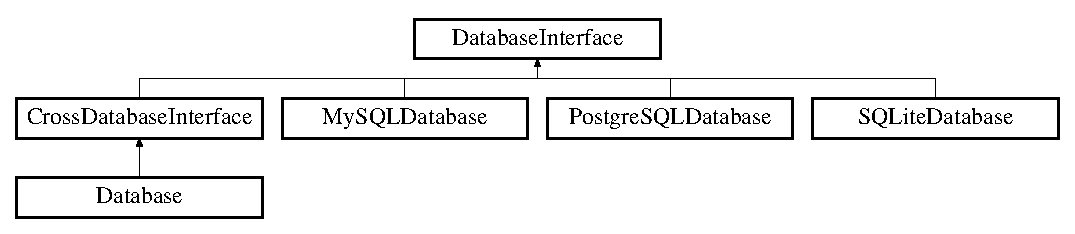
\includegraphics[height=1.794872cm]{interface_database_interface}
\end{center}
\end{figure}
\subsection*{Public Member Functions}
\begin{DoxyCompactItemize}
\item 
\hyperlink{interface_database_interface_a4717bbfc70a40a57ee741ed70766c309}{\+\_\+\+\_\+construct} (\$name)
\item 
\hyperlink{interface_database_interface_a9aac7e1475efe923de4e19cc2511f092}{\+\_\+\+\_\+invoke} ()
\item 
\hyperlink{interface_database_interface_a7516ca30af0db3cdbf9a7739b48ce91d}{\+\_\+\+\_\+to\+String} ()
\item 
\hyperlink{interface_database_interface_a0205d4089913613e23189c60d7fdf89a}{column\+Exists} ()
\item 
\hyperlink{interface_database_interface_a6287262cb9628d7a89d8fc16dcb51177}{get\+Columns} ()
\item 
\hyperlink{interface_database_interface_af54c3eed64c3e3dfb06a2541289ff0da}{get\+Default\+Table} ()
\item 
\hyperlink{interface_database_interface_a61b9097ace78236a1a7f9cfd9e9ab01c}{get\+Tables} ()
\item 
\hyperlink{interface_database_interface_ad0aa1804fc79c22b46596db136320017}{has\+Default\+Table} ()
\item 
\hyperlink{interface_database_interface_a8e5626f114925dee9986c8edbfc3ec05}{insert} (\$in, \$table=null)
\item 
\hyperlink{interface_database_interface_a1efc6b974510d4c668660f1abe184182}{select} (\$columns=\mbox{[}\textquotesingle{}$\ast$\textquotesingle{}\mbox{]}, \$conditions=null, \$start=null, \$count=null, \$sort\+By=null, \$sort\+Direction=null, \$table=null)
\item 
\hyperlink{interface_database_interface_ae7cdaa744d52a1eb0103e377023ca528}{table\+Exists} (\$table)
\item 
\hyperlink{interface_database_interface_a3211e273c3ee674b966bab63d966c4b2}{update} (\$array)
\end{DoxyCompactItemize}


\subsection{Detailed Description}


Definition at line 3 of file Database\+Interface.\+php.



\subsection{Constructor \& Destructor Documentation}
\hypertarget{interface_database_interface_a4717bbfc70a40a57ee741ed70766c309}{}\index{Database\+Interface@{Database\+Interface}!\+\_\+\+\_\+construct@{\+\_\+\+\_\+construct}}
\index{\+\_\+\+\_\+construct@{\+\_\+\+\_\+construct}!Database\+Interface@{Database\+Interface}}
\subsubsection[{\+\_\+\+\_\+construct}]{\setlength{\rightskip}{0pt plus 5cm}\+\_\+\+\_\+construct (
\begin{DoxyParamCaption}
\item[{}]{\$name}
\end{DoxyParamCaption}
)}\label{interface_database_interface_a4717bbfc70a40a57ee741ed70766c309}


\subsection{Member Function Documentation}
\hypertarget{interface_database_interface_a9aac7e1475efe923de4e19cc2511f092}{}\index{Database\+Interface@{Database\+Interface}!\+\_\+\+\_\+invoke@{\+\_\+\+\_\+invoke}}
\index{\+\_\+\+\_\+invoke@{\+\_\+\+\_\+invoke}!Database\+Interface@{Database\+Interface}}
\subsubsection[{\+\_\+\+\_\+invoke}]{\setlength{\rightskip}{0pt plus 5cm}\+\_\+\+\_\+invoke (
\begin{DoxyParamCaption}
{}
\end{DoxyParamCaption}
)}\label{interface_database_interface_a9aac7e1475efe923de4e19cc2511f092}


Implemented in \hyperlink{class_my_s_q_l_database_a9aac7e1475efe923de4e19cc2511f092}{My\+S\+Q\+L\+Database}, and \hyperlink{class_database_a9aac7e1475efe923de4e19cc2511f092}{Database}.

\hypertarget{interface_database_interface_a7516ca30af0db3cdbf9a7739b48ce91d}{}\index{Database\+Interface@{Database\+Interface}!\+\_\+\+\_\+to\+String@{\+\_\+\+\_\+to\+String}}
\index{\+\_\+\+\_\+to\+String@{\+\_\+\+\_\+to\+String}!Database\+Interface@{Database\+Interface}}
\subsubsection[{\+\_\+\+\_\+to\+String}]{\setlength{\rightskip}{0pt plus 5cm}\+\_\+\+\_\+to\+String (
\begin{DoxyParamCaption}
{}
\end{DoxyParamCaption}
)}\label{interface_database_interface_a7516ca30af0db3cdbf9a7739b48ce91d}


Implemented in \hyperlink{class_my_s_q_l_database_a7516ca30af0db3cdbf9a7739b48ce91d}{My\+S\+Q\+L\+Database}, and \hyperlink{class_database_a7516ca30af0db3cdbf9a7739b48ce91d}{Database}.

\hypertarget{interface_database_interface_a0205d4089913613e23189c60d7fdf89a}{}\index{Database\+Interface@{Database\+Interface}!column\+Exists@{column\+Exists}}
\index{column\+Exists@{column\+Exists}!Database\+Interface@{Database\+Interface}}
\subsubsection[{column\+Exists}]{\setlength{\rightskip}{0pt plus 5cm}column\+Exists (
\begin{DoxyParamCaption}
{}
\end{DoxyParamCaption}
)}\label{interface_database_interface_a0205d4089913613e23189c60d7fdf89a}
\hypertarget{interface_database_interface_a6287262cb9628d7a89d8fc16dcb51177}{}\index{Database\+Interface@{Database\+Interface}!get\+Columns@{get\+Columns}}
\index{get\+Columns@{get\+Columns}!Database\+Interface@{Database\+Interface}}
\subsubsection[{get\+Columns}]{\setlength{\rightskip}{0pt plus 5cm}get\+Columns (
\begin{DoxyParamCaption}
{}
\end{DoxyParamCaption}
)}\label{interface_database_interface_a6287262cb9628d7a89d8fc16dcb51177}
\hypertarget{interface_database_interface_af54c3eed64c3e3dfb06a2541289ff0da}{}\index{Database\+Interface@{Database\+Interface}!get\+Default\+Table@{get\+Default\+Table}}
\index{get\+Default\+Table@{get\+Default\+Table}!Database\+Interface@{Database\+Interface}}
\subsubsection[{get\+Default\+Table}]{\setlength{\rightskip}{0pt plus 5cm}get\+Default\+Table (
\begin{DoxyParamCaption}
{}
\end{DoxyParamCaption}
)}\label{interface_database_interface_af54c3eed64c3e3dfb06a2541289ff0da}


Implemented in \hyperlink{class_my_s_q_l_database_af54c3eed64c3e3dfb06a2541289ff0da}{My\+S\+Q\+L\+Database}, and \hyperlink{class_database_af54c3eed64c3e3dfb06a2541289ff0da}{Database}.

\hypertarget{interface_database_interface_a61b9097ace78236a1a7f9cfd9e9ab01c}{}\index{Database\+Interface@{Database\+Interface}!get\+Tables@{get\+Tables}}
\index{get\+Tables@{get\+Tables}!Database\+Interface@{Database\+Interface}}
\subsubsection[{get\+Tables}]{\setlength{\rightskip}{0pt plus 5cm}get\+Tables (
\begin{DoxyParamCaption}
{}
\end{DoxyParamCaption}
)}\label{interface_database_interface_a61b9097ace78236a1a7f9cfd9e9ab01c}


Implemented in \hyperlink{class_my_s_q_l_database_a61b9097ace78236a1a7f9cfd9e9ab01c}{My\+S\+Q\+L\+Database}, and \hyperlink{class_database_a61b9097ace78236a1a7f9cfd9e9ab01c}{Database}.

\hypertarget{interface_database_interface_ad0aa1804fc79c22b46596db136320017}{}\index{Database\+Interface@{Database\+Interface}!has\+Default\+Table@{has\+Default\+Table}}
\index{has\+Default\+Table@{has\+Default\+Table}!Database\+Interface@{Database\+Interface}}
\subsubsection[{has\+Default\+Table}]{\setlength{\rightskip}{0pt plus 5cm}has\+Default\+Table (
\begin{DoxyParamCaption}
{}
\end{DoxyParamCaption}
)}\label{interface_database_interface_ad0aa1804fc79c22b46596db136320017}


Implemented in \hyperlink{class_my_s_q_l_database_ad0aa1804fc79c22b46596db136320017}{My\+S\+Q\+L\+Database}, and \hyperlink{class_database_ad0aa1804fc79c22b46596db136320017}{Database}.

\hypertarget{interface_database_interface_a8e5626f114925dee9986c8edbfc3ec05}{}\index{Database\+Interface@{Database\+Interface}!insert@{insert}}
\index{insert@{insert}!Database\+Interface@{Database\+Interface}}
\subsubsection[{insert}]{\setlength{\rightskip}{0pt plus 5cm}insert (
\begin{DoxyParamCaption}
\item[{}]{\$in, }
\item[{}]{\$table = {\ttfamily null}}
\end{DoxyParamCaption}
)}\label{interface_database_interface_a8e5626f114925dee9986c8edbfc3ec05}


Implemented in \hyperlink{class_my_s_q_l_database_a8e5626f114925dee9986c8edbfc3ec05}{My\+S\+Q\+L\+Database}, and \hyperlink{class_database_a8e5626f114925dee9986c8edbfc3ec05}{Database}.

\hypertarget{interface_database_interface_a1efc6b974510d4c668660f1abe184182}{}\index{Database\+Interface@{Database\+Interface}!select@{select}}
\index{select@{select}!Database\+Interface@{Database\+Interface}}
\subsubsection[{select}]{\setlength{\rightskip}{0pt plus 5cm}select (
\begin{DoxyParamCaption}
\item[{}]{\$columns = {\ttfamily \mbox{[}\textquotesingle{}$\ast$\textquotesingle{}\mbox{]}}, }
\item[{}]{\$conditions = {\ttfamily null}, }
\item[{}]{\$start = {\ttfamily null}, }
\item[{}]{\$count = {\ttfamily null}, }
\item[{}]{\$sort\+By = {\ttfamily null}, }
\item[{}]{\$sort\+Direction = {\ttfamily null}, }
\item[{}]{\$table = {\ttfamily null}}
\end{DoxyParamCaption}
)}\label{interface_database_interface_a1efc6b974510d4c668660f1abe184182}


Implemented in \hyperlink{class_my_s_q_l_database_a1efc6b974510d4c668660f1abe184182}{My\+S\+Q\+L\+Database}, and \hyperlink{class_database_a1efc6b974510d4c668660f1abe184182}{Database}.

\hypertarget{interface_database_interface_ae7cdaa744d52a1eb0103e377023ca528}{}\index{Database\+Interface@{Database\+Interface}!table\+Exists@{table\+Exists}}
\index{table\+Exists@{table\+Exists}!Database\+Interface@{Database\+Interface}}
\subsubsection[{table\+Exists}]{\setlength{\rightskip}{0pt plus 5cm}table\+Exists (
\begin{DoxyParamCaption}
\item[{}]{\$table}
\end{DoxyParamCaption}
)}\label{interface_database_interface_ae7cdaa744d52a1eb0103e377023ca528}


Implemented in \hyperlink{class_my_s_q_l_database_ae7cdaa744d52a1eb0103e377023ca528}{My\+S\+Q\+L\+Database}, and \hyperlink{class_database_ae7cdaa744d52a1eb0103e377023ca528}{Database}.

\hypertarget{interface_database_interface_a3211e273c3ee674b966bab63d966c4b2}{}\index{Database\+Interface@{Database\+Interface}!update@{update}}
\index{update@{update}!Database\+Interface@{Database\+Interface}}
\subsubsection[{update}]{\setlength{\rightskip}{0pt plus 5cm}update (
\begin{DoxyParamCaption}
\item[{}]{\$array}
\end{DoxyParamCaption}
)}\label{interface_database_interface_a3211e273c3ee674b966bab63d966c4b2}


The documentation for this interface was generated from the following file\+:\begin{DoxyCompactItemize}
\item 
src/class/\hyperlink{_database_interface_8php}{Database\+Interface.\+php}\end{DoxyCompactItemize}

\hypertarget{class_database_utils}{}\section{Database\+Utils Class Reference}
\label{class_database_utils}\index{Database\+Utils@{Database\+Utils}}
\subsection*{Static Public Member Functions}
\begin{DoxyCompactItemize}
\item 
static \hyperlink{class_database_utils_a2aeb4c5320456b64219630c839470713}{array\+Depth} (array \$array)
\item 
static \hyperlink{class_database_utils_a0ceab1ee918d680c3996af0a5ced6e8c}{is\+Valid\+Host} (\$host)
\item 
static \hyperlink{class_database_utils_ac070c2b36a0c7c929da708906b269bd7}{recurse\+Array} (array \$array, callable \$function)
\end{DoxyCompactItemize}


\subsection{Detailed Description}


Definition at line 3 of file Database\+Utils.\+php.



\subsection{Member Function Documentation}
\hypertarget{class_database_utils_a2aeb4c5320456b64219630c839470713}{}\index{Database\+Utils@{Database\+Utils}!array\+Depth@{array\+Depth}}
\index{array\+Depth@{array\+Depth}!Database\+Utils@{Database\+Utils}}
\subsubsection[{array\+Depth}]{\setlength{\rightskip}{0pt plus 5cm}static array\+Depth (
\begin{DoxyParamCaption}
\item[{array}]{\$array}
\end{DoxyParamCaption}
)\hspace{0.3cm}{\ttfamily [static]}}\label{class_database_utils_a2aeb4c5320456b64219630c839470713}
\hyperlink{class_database_utils_a2aeb4c5320456b64219630c839470713}{Database\+Utils\+::array\+Depth()} Static Method

calculates depth of an array (how many nested arrays need/can be traversed)


\begin{DoxyParams}[1]{Parameters}
array & {\em \$array} & -\/ Array on which to calculate depth \\
\hline
\end{DoxyParams}
\begin{DoxyReturn}{Returns}
integer -\/ Maximum depth of the array 
\end{DoxyReturn}


Definition at line 13 of file Database\+Utils.\+php.

\hypertarget{class_database_utils_a0ceab1ee918d680c3996af0a5ced6e8c}{}\index{Database\+Utils@{Database\+Utils}!is\+Valid\+Host@{is\+Valid\+Host}}
\index{is\+Valid\+Host@{is\+Valid\+Host}!Database\+Utils@{Database\+Utils}}
\subsubsection[{is\+Valid\+Host}]{\setlength{\rightskip}{0pt plus 5cm}static is\+Valid\+Host (
\begin{DoxyParamCaption}
\item[{}]{\$host}
\end{DoxyParamCaption}
)\hspace{0.3cm}{\ttfamily [static]}}\label{class_database_utils_a0ceab1ee918d680c3996af0a5ced6e8c}
\hyperlink{class_database_utils_a0ceab1ee918d680c3996af0a5ced6e8c}{Database\+Utils\+::is\+Valid\+Host()} Static Method

tests if a string is a valid I\+P address or hostname.


\begin{DoxyParams}[1]{Parameters}
string & {\em \$host} & (required) -\/ hostname/ip-\/address to test \\
\hline
\end{DoxyParams}
\begin{DoxyReturn}{Returns}
boolean -\/ is it valid (true) or not (false)? 
\end{DoxyReturn}


Definition at line 38 of file Database\+Utils.\+php.

\hypertarget{class_database_utils_ac070c2b36a0c7c929da708906b269bd7}{}\index{Database\+Utils@{Database\+Utils}!recurse\+Array@{recurse\+Array}}
\index{recurse\+Array@{recurse\+Array}!Database\+Utils@{Database\+Utils}}
\subsubsection[{recurse\+Array}]{\setlength{\rightskip}{0pt plus 5cm}static recurse\+Array (
\begin{DoxyParamCaption}
\item[{array}]{\$array, }
\item[{callable}]{\$function}
\end{DoxyParamCaption}
)\hspace{0.3cm}{\ttfamily [static]}}\label{class_database_utils_ac070c2b36a0c7c929da708906b269bd7}


Definition at line 87 of file Database\+Utils.\+php.



The documentation for this class was generated from the following file\+:\begin{DoxyCompactItemize}
\item 
src/class/\hyperlink{_database_utils_8php}{Database\+Utils.\+php}\end{DoxyCompactItemize}

\hypertarget{class_my_s_q_l_condition}{}\section{My\+S\+Q\+L\+Condition Class Reference}
\label{class_my_s_q_l_condition}\index{My\+S\+Q\+L\+Condition@{My\+S\+Q\+L\+Condition}}
Inheritance diagram for My\+S\+Q\+L\+Condition\+:\begin{figure}[H]
\begin{center}
\leavevmode
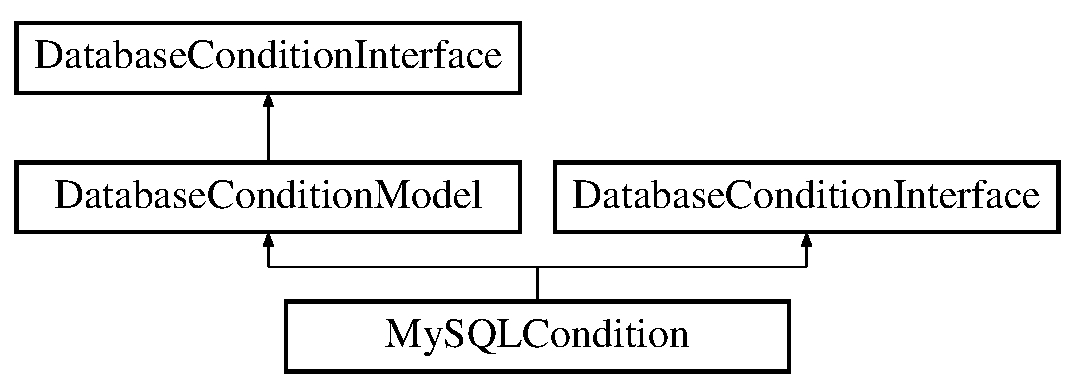
\includegraphics[height=3.000000cm]{class_my_s_q_l_condition}
\end{center}
\end{figure}
\subsection*{Additional Inherited Members}


\subsection{Detailed Description}


Definition at line 3 of file My\+S\+Q\+L\+Condition.\+php.



The documentation for this class was generated from the following file\+:\begin{DoxyCompactItemize}
\item 
src/class/\hyperlink{_my_s_q_l_condition_8php}{My\+S\+Q\+L\+Condition.\+php}\end{DoxyCompactItemize}

\hypertarget{class_my_s_q_l_database}{}\section{My\+S\+Q\+L\+Database Class Reference}
\label{class_my_s_q_l_database}\index{My\+S\+Q\+L\+Database@{My\+S\+Q\+L\+Database}}
Inheritance diagram for My\+S\+Q\+L\+Database\+:\begin{figure}[H]
\begin{center}
\leavevmode
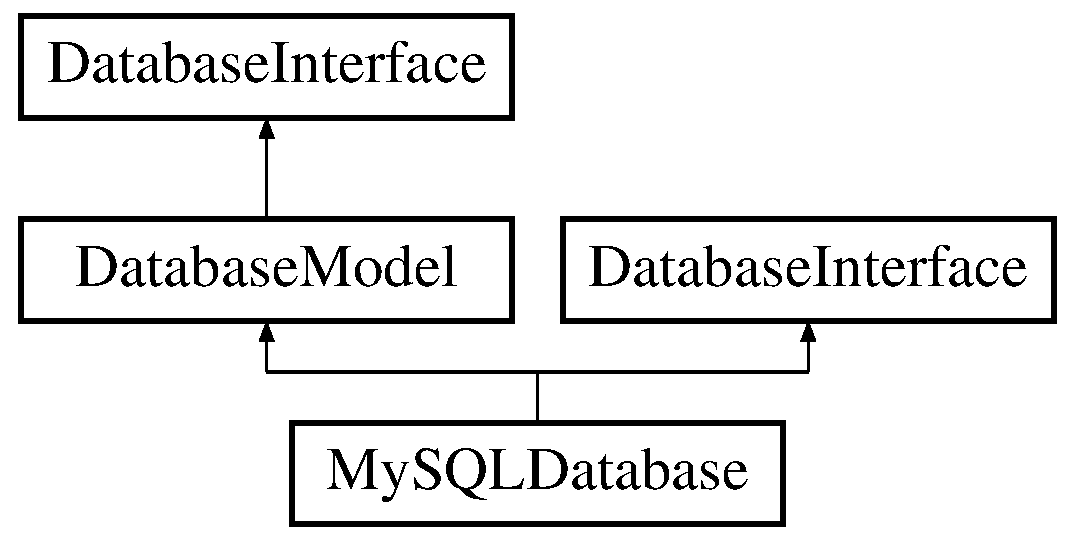
\includegraphics[height=3.000000cm]{class_my_s_q_l_database}
\end{center}
\end{figure}
\subsection*{Public Member Functions}
\begin{DoxyCompactItemize}
\item 
\hyperlink{class_my_s_q_l_database_a522739237db8d43369172cfe07bf7b85}{\+\_\+\+\_\+construct} (\$name, \$user=null, \$pass=null, \$host= \textquotesingle{}localhost\textquotesingle{}, \$port=null, \$table=null)
\item 
\hyperlink{class_my_s_q_l_database_a421831a265621325e1fdd19aace0c758}{\+\_\+\+\_\+destruct} ()
\item 
\hyperlink{class_my_s_q_l_database_a9aac7e1475efe923de4e19cc2511f092}{\+\_\+\+\_\+invoke} ()
\item 
\hyperlink{class_my_s_q_l_database_a7516ca30af0db3cdbf9a7739b48ce91d}{\+\_\+\+\_\+to\+String} ()
\item 
\hyperlink{class_my_s_q_l_database_a42c4cefdb183a7caa3115193a811d893}{column\+Exists} (\$column, \$table=null)
\item 
\hyperlink{class_my_s_q_l_database_a5cc0962e790b9ccffd2ca9c77cead320}{get\+Columns} (\$table=null)
\item 
\hyperlink{class_my_s_q_l_database_af54c3eed64c3e3dfb06a2541289ff0da}{get\+Default\+Table} ()
\item 
\hyperlink{class_my_s_q_l_database_a61b9097ace78236a1a7f9cfd9e9ab01c}{get\+Tables} ()
\item 
\hyperlink{class_my_s_q_l_database_a830b5c75df72b32396701bc563fbe3c7}{get\+Type} ()
\item 
\hyperlink{class_my_s_q_l_database_ad0aa1804fc79c22b46596db136320017}{has\+Default\+Table} ()
\item 
\hyperlink{class_my_s_q_l_database_a8e5626f114925dee9986c8edbfc3ec05}{insert} (\$in, \$table=null)
\item 
\& \hyperlink{class_my_s_q_l_database_ae6979f06c8e38dbe758ff53f7395531f}{ref} ()
\item 
\hyperlink{class_my_s_q_l_database_a1efc6b974510d4c668660f1abe184182}{select} (\$columns=\mbox{[}\textquotesingle{}$\ast$\textquotesingle{}\mbox{]}, \$conditions=null, \$start=null, \$count=null, \$sort\+By=null, \$sort\+Direction=null, \$table=null)
\item 
\hyperlink{class_my_s_q_l_database_ae7cdaa744d52a1eb0103e377023ca528}{table\+Exists} (\$table)
\end{DoxyCompactItemize}
\subsection*{Data Fields}
\begin{DoxyCompactItemize}
\item 
const \hyperlink{class_my_s_q_l_database_ac3188f4350978425c488580c5cea8468}{F\+I\+E\+L\+D\+\_\+\+D\+A\+T\+A} = 0
\item 
const \hyperlink{class_my_s_q_l_database_acbdf154a35cfc228dd1016e8aa4bd503}{F\+I\+E\+L\+D\+\_\+\+T\+A\+B\+L\+E} = 1
\item 
const \hyperlink{class_my_s_q_l_database_a87aad3e89cc6a17f293cf5410b225bbe}{F\+I\+E\+L\+D\+\_\+\+C\+O\+L\+U\+M\+N} = 2
\item 
const \hyperlink{class_my_s_q_l_database_a9b1a24ef01d468c146a71b333edb0c17}{K\+E\+Y\+W\+O\+R\+D\+\_\+\+N\+O\+N\+E} = 0
\item 
const \hyperlink{class_my_s_q_l_database_ababb5c4af464938f3f0b8f9c4fa183ba}{K\+E\+Y\+W\+O\+R\+D\+\_\+\+A\+L\+L} = 1
\item 
const \hyperlink{class_my_s_q_l_database_af3826c676cb54905f393f9d1f7ad48ea}{S\+O\+R\+T\+\_\+\+N\+O\+N\+E} = 0
\item 
const \hyperlink{class_my_s_q_l_database_a9517f2622dfc5fbb0cc64feef247eb06}{S\+O\+R\+T\+\_\+\+A\+S\+C} = 1
\item 
const \hyperlink{class_my_s_q_l_database_a0e633ab431ae1e5cc483a37cfe73bb09}{S\+O\+R\+T\+\_\+\+D\+E\+S\+C} = 2
\end{DoxyCompactItemize}
\subsection*{Protected Attributes}
\begin{DoxyCompactItemize}
\item 
\hyperlink{class_my_s_q_l_database_a49c7011be9c979d9174c52a8b83e5d8e}{\$config}
\item 
\hyperlink{class_my_s_q_l_database_a7c7a1968b87fd4d016e364b27b7a3d7d}{\$connector}
\item 
\hyperlink{class_my_s_q_l_database_aee271b7ce67fbe00b9976e6c347cbfbf}{\$encoding}
\item 
\hyperlink{class_my_s_q_l_database_a711797613cb863ca0756df789c396bf2}{\$host}
\item 
\hyperlink{class_my_s_q_l_database_ae19722790c6683980bbf0af8572f26ab}{\$info}
\item 
\hyperlink{class_my_s_q_l_database_a6cb6be70a528323568af007db6a3885e}{\$last\+Error}
\item 
\hyperlink{class_my_s_q_l_database_a12ff8f78a47e0fa691355a485c2e696a}{\$last\+Stack\+Trace}
\item 
\hyperlink{class_my_s_q_l_database_ab2fc40d43824ea3e1ce5d86dee0d763b}{\$name}
\item 
\hyperlink{class_my_s_q_l_database_a4269f690c0554ecb1deec21b80f321dc}{\$open}
\item 
\hyperlink{class_my_s_q_l_database_aa0787efab4b22e8a212882f3409d4c77}{\$port}
\item 
\hyperlink{class_my_s_q_l_database_ae8876a14058f368335baccf35af4a22b}{\$table}
\end{DoxyCompactItemize}


\subsection{Detailed Description}


Definition at line 3 of file My\+S\+Q\+L\+Database.\+php.



\subsection{Constructor \& Destructor Documentation}
\hypertarget{class_my_s_q_l_database_a522739237db8d43369172cfe07bf7b85}{}\index{My\+S\+Q\+L\+Database@{My\+S\+Q\+L\+Database}!\+\_\+\+\_\+construct@{\+\_\+\+\_\+construct}}
\index{\+\_\+\+\_\+construct@{\+\_\+\+\_\+construct}!My\+S\+Q\+L\+Database@{My\+S\+Q\+L\+Database}}
\subsubsection[{\+\_\+\+\_\+construct}]{\setlength{\rightskip}{0pt plus 5cm}\+\_\+\+\_\+construct (
\begin{DoxyParamCaption}
\item[{}]{\$name, }
\item[{}]{\$user = {\ttfamily null}, }
\item[{}]{\$pass = {\ttfamily null}, }
\item[{}]{\$host = {\ttfamily \textquotesingle{}localhost\textquotesingle{}}, }
\item[{}]{\$port = {\ttfamily null}, }
\item[{}]{\$table = {\ttfamily null}}
\end{DoxyParamCaption}
)}\label{class_my_s_q_l_database_a522739237db8d43369172cfe07bf7b85}
Constructor Method 
\begin{DoxyParams}[1]{Parameters}
int & {\em \$type} & (required) -\/ \\
\hline
string & {\em \$name} & (required) -\/ \\
\hline
string & {\em \$user} & (required for secured) -\/ \\
\hline
string & {\em \$pass} & (required for secured) -\/ \\
\hline
string & {\em \$host} & (required for remote, optional because it defaults to localhost) -\/ \\
\hline
integer & {\em \$port} & (required for remote, optional because it defaults to server type\textquotesingle{}s default port) -\/ \\
\hline
strign & {\em \$table} & (optional) -\/ \\
\hline
\end{DoxyParams}


Definition at line 45 of file My\+S\+Q\+L\+Database.\+php.

\hypertarget{class_my_s_q_l_database_a421831a265621325e1fdd19aace0c758}{}\index{My\+S\+Q\+L\+Database@{My\+S\+Q\+L\+Database}!\+\_\+\+\_\+destruct@{\+\_\+\+\_\+destruct}}
\index{\+\_\+\+\_\+destruct@{\+\_\+\+\_\+destruct}!My\+S\+Q\+L\+Database@{My\+S\+Q\+L\+Database}}
\subsubsection[{\+\_\+\+\_\+destruct}]{\setlength{\rightskip}{0pt plus 5cm}\+\_\+\+\_\+destruct (
\begin{DoxyParamCaption}
{}
\end{DoxyParamCaption}
)}\label{class_my_s_q_l_database_a421831a265621325e1fdd19aace0c758}
Destructor Method 

Definition at line 263 of file My\+S\+Q\+L\+Database.\+php.



\subsection{Member Function Documentation}
\hypertarget{class_my_s_q_l_database_a9aac7e1475efe923de4e19cc2511f092}{}\index{My\+S\+Q\+L\+Database@{My\+S\+Q\+L\+Database}!\+\_\+\+\_\+invoke@{\+\_\+\+\_\+invoke}}
\index{\+\_\+\+\_\+invoke@{\+\_\+\+\_\+invoke}!My\+S\+Q\+L\+Database@{My\+S\+Q\+L\+Database}}
\subsubsection[{\+\_\+\+\_\+invoke}]{\setlength{\rightskip}{0pt plus 5cm}\+\_\+\+\_\+invoke (
\begin{DoxyParamCaption}
{}
\end{DoxyParamCaption}
)}\label{class_my_s_q_l_database_a9aac7e1475efe923de4e19cc2511f092}
Invocation Method 

Implements \hyperlink{interface_database_interface_a9aac7e1475efe923de4e19cc2511f092}{Database\+Interface}.



Definition at line 272 of file My\+S\+Q\+L\+Database.\+php.

\hypertarget{class_my_s_q_l_database_a7516ca30af0db3cdbf9a7739b48ce91d}{}\index{My\+S\+Q\+L\+Database@{My\+S\+Q\+L\+Database}!\+\_\+\+\_\+to\+String@{\+\_\+\+\_\+to\+String}}
\index{\+\_\+\+\_\+to\+String@{\+\_\+\+\_\+to\+String}!My\+S\+Q\+L\+Database@{My\+S\+Q\+L\+Database}}
\subsubsection[{\+\_\+\+\_\+to\+String}]{\setlength{\rightskip}{0pt plus 5cm}\+\_\+\+\_\+to\+String (
\begin{DoxyParamCaption}
{}
\end{DoxyParamCaption}
)}\label{class_my_s_q_l_database_a7516ca30af0db3cdbf9a7739b48ce91d}
String Conversion Method 

Implements \hyperlink{interface_database_interface_a7516ca30af0db3cdbf9a7739b48ce91d}{Database\+Interface}.



Definition at line 281 of file My\+S\+Q\+L\+Database.\+php.

\hypertarget{class_my_s_q_l_database_a42c4cefdb183a7caa3115193a811d893}{}\index{My\+S\+Q\+L\+Database@{My\+S\+Q\+L\+Database}!column\+Exists@{column\+Exists}}
\index{column\+Exists@{column\+Exists}!My\+S\+Q\+L\+Database@{My\+S\+Q\+L\+Database}}
\subsubsection[{column\+Exists}]{\setlength{\rightskip}{0pt plus 5cm}column\+Exists (
\begin{DoxyParamCaption}
\item[{}]{\$column, }
\item[{}]{\$table = {\ttfamily null}}
\end{DoxyParamCaption}
)}\label{class_my_s_q_l_database_a42c4cefdb183a7caa3115193a811d893}


Definition at line 287 of file My\+S\+Q\+L\+Database.\+php.

\hypertarget{class_my_s_q_l_database_a5cc0962e790b9ccffd2ca9c77cead320}{}\index{My\+S\+Q\+L\+Database@{My\+S\+Q\+L\+Database}!get\+Columns@{get\+Columns}}
\index{get\+Columns@{get\+Columns}!My\+S\+Q\+L\+Database@{My\+S\+Q\+L\+Database}}
\subsubsection[{get\+Columns}]{\setlength{\rightskip}{0pt plus 5cm}get\+Columns (
\begin{DoxyParamCaption}
\item[{}]{\$table = {\ttfamily null}}
\end{DoxyParamCaption}
)}\label{class_my_s_q_l_database_a5cc0962e790b9ccffd2ca9c77cead320}
Database-\/$>$\hyperlink{interface_database_interface_a6287262cb9628d7a89d8fc16dcb51177}{get\+Columns()} Method


\begin{DoxyParams}[1]{Parameters}
string & {\em \$table} & (optional) -\/ name of table, unless table defined by constructor \\
\hline
\end{DoxyParams}
\begin{DoxyReturn}{Returns}
array -\/ array of columns in the table 
\end{DoxyReturn}


Definition at line 378 of file My\+S\+Q\+L\+Database.\+php.

\hypertarget{class_my_s_q_l_database_af54c3eed64c3e3dfb06a2541289ff0da}{}\index{My\+S\+Q\+L\+Database@{My\+S\+Q\+L\+Database}!get\+Default\+Table@{get\+Default\+Table}}
\index{get\+Default\+Table@{get\+Default\+Table}!My\+S\+Q\+L\+Database@{My\+S\+Q\+L\+Database}}
\subsubsection[{get\+Default\+Table}]{\setlength{\rightskip}{0pt plus 5cm}get\+Default\+Table (
\begin{DoxyParamCaption}
{}
\end{DoxyParamCaption}
)}\label{class_my_s_q_l_database_af54c3eed64c3e3dfb06a2541289ff0da}


Implements \hyperlink{interface_database_interface_af54c3eed64c3e3dfb06a2541289ff0da}{Database\+Interface}.



Definition at line 427 of file My\+S\+Q\+L\+Database.\+php.

\hypertarget{class_my_s_q_l_database_a61b9097ace78236a1a7f9cfd9e9ab01c}{}\index{My\+S\+Q\+L\+Database@{My\+S\+Q\+L\+Database}!get\+Tables@{get\+Tables}}
\index{get\+Tables@{get\+Tables}!My\+S\+Q\+L\+Database@{My\+S\+Q\+L\+Database}}
\subsubsection[{get\+Tables}]{\setlength{\rightskip}{0pt plus 5cm}get\+Tables (
\begin{DoxyParamCaption}
{}
\end{DoxyParamCaption}
)}\label{class_my_s_q_l_database_a61b9097ace78236a1a7f9cfd9e9ab01c}


Implements \hyperlink{interface_database_interface_a61b9097ace78236a1a7f9cfd9e9ab01c}{Database\+Interface}.



Definition at line 433 of file My\+S\+Q\+L\+Database.\+php.

\hypertarget{class_my_s_q_l_database_a830b5c75df72b32396701bc563fbe3c7}{}\index{My\+S\+Q\+L\+Database@{My\+S\+Q\+L\+Database}!get\+Type@{get\+Type}}
\index{get\+Type@{get\+Type}!My\+S\+Q\+L\+Database@{My\+S\+Q\+L\+Database}}
\subsubsection[{get\+Type}]{\setlength{\rightskip}{0pt plus 5cm}get\+Type (
\begin{DoxyParamCaption}
{}
\end{DoxyParamCaption}
)}\label{class_my_s_q_l_database_a830b5c75df72b32396701bc563fbe3c7}
Database-\/$>$\hyperlink{class_my_s_q_l_database_a830b5c75df72b32396701bc563fbe3c7}{get\+Type()} Getter Method \begin{DoxyReturn}{Returns}
string \$this-\/$>$type 
\end{DoxyReturn}


Definition at line 466 of file My\+S\+Q\+L\+Database.\+php.

\hypertarget{class_my_s_q_l_database_ad0aa1804fc79c22b46596db136320017}{}\index{My\+S\+Q\+L\+Database@{My\+S\+Q\+L\+Database}!has\+Default\+Table@{has\+Default\+Table}}
\index{has\+Default\+Table@{has\+Default\+Table}!My\+S\+Q\+L\+Database@{My\+S\+Q\+L\+Database}}
\subsubsection[{has\+Default\+Table}]{\setlength{\rightskip}{0pt plus 5cm}has\+Default\+Table (
\begin{DoxyParamCaption}
{}
\end{DoxyParamCaption}
)}\label{class_my_s_q_l_database_ad0aa1804fc79c22b46596db136320017}


Implements \hyperlink{interface_database_interface_ad0aa1804fc79c22b46596db136320017}{Database\+Interface}.



Definition at line 472 of file My\+S\+Q\+L\+Database.\+php.

\hypertarget{class_my_s_q_l_database_a8e5626f114925dee9986c8edbfc3ec05}{}\index{My\+S\+Q\+L\+Database@{My\+S\+Q\+L\+Database}!insert@{insert}}
\index{insert@{insert}!My\+S\+Q\+L\+Database@{My\+S\+Q\+L\+Database}}
\subsubsection[{insert}]{\setlength{\rightskip}{0pt plus 5cm}insert (
\begin{DoxyParamCaption}
\item[{}]{\$in, }
\item[{}]{\$table = {\ttfamily null}}
\end{DoxyParamCaption}
)}\label{class_my_s_q_l_database_a8e5626f114925dee9986c8edbfc3ec05}
Database-\/$>$\hyperlink{class_my_s_q_l_database_a8e5626f114925dee9986c8edbfc3ec05}{insert()} Method


\begin{DoxyParams}[1]{Parameters}
array & {\em \$in} & (required) -\/ associative array of input to be inserted, keys being the name of columns \\
\hline
string & {\em \$table} & (optional if defined in constructor) -\/ table to use \\
\hline
\end{DoxyParams}
\begin{DoxyReturn}{Returns}
\hyperlink{class_database}{Database} -\/ reference to self 
\end{DoxyReturn}


Implements \hyperlink{interface_database_interface_a8e5626f114925dee9986c8edbfc3ec05}{Database\+Interface}.



Definition at line 489 of file My\+S\+Q\+L\+Database.\+php.

\hypertarget{class_my_s_q_l_database_ae6979f06c8e38dbe758ff53f7395531f}{}\index{My\+S\+Q\+L\+Database@{My\+S\+Q\+L\+Database}!ref@{ref}}
\index{ref@{ref}!My\+S\+Q\+L\+Database@{My\+S\+Q\+L\+Database}}
\subsubsection[{ref}]{\setlength{\rightskip}{0pt plus 5cm}\& ref (
\begin{DoxyParamCaption}
{}
\end{DoxyParamCaption}
)}\label{class_my_s_q_l_database_ae6979f06c8e38dbe758ff53f7395531f}
Self Reference Method \begin{DoxyReturn}{Returns}
\hyperlink{class_database}{Database} 
\end{DoxyReturn}


Definition at line 625 of file My\+S\+Q\+L\+Database.\+php.

\hypertarget{class_my_s_q_l_database_a1efc6b974510d4c668660f1abe184182}{}\index{My\+S\+Q\+L\+Database@{My\+S\+Q\+L\+Database}!select@{select}}
\index{select@{select}!My\+S\+Q\+L\+Database@{My\+S\+Q\+L\+Database}}
\subsubsection[{select}]{\setlength{\rightskip}{0pt plus 5cm}select (
\begin{DoxyParamCaption}
\item[{}]{\$columns = {\ttfamily \mbox{[}\textquotesingle{}$\ast$\textquotesingle{}\mbox{]}}, }
\item[{}]{\$conditions = {\ttfamily null}, }
\item[{}]{\$start = {\ttfamily null}, }
\item[{}]{\$count = {\ttfamily null}, }
\item[{}]{\$sort\+By = {\ttfamily null}, }
\item[{}]{\$sort\+Direction = {\ttfamily null}, }
\item[{}]{\$table = {\ttfamily null}}
\end{DoxyParamCaption}
)}\label{class_my_s_q_l_database_a1efc6b974510d4c668660f1abe184182}
Database-\/$>$\hyperlink{class_my_s_q_l_database_a1efc6b974510d4c668660f1abe184182}{select()} Method


\begin{DoxyParams}[1]{Parameters}
array | string & {\em \$columns} & (optional) -\/ columns to return. if left empty/null, will default to all columns ($\ast$) \\
\hline
Database\+Condition | array | string & {\em \$conditions} & (optional) -\/ conditions to lookup. If left empty/null, will default to no conditions. \\
\hline
int & {\em \$start} & (optional) -\/ starting index from which to begin selecting. If left empty, defaults to 0. \\
\hline
int & {\em \$count} & (optional) -\/ maximum number of results to return. If left empty, defaults to no limit. \\
\hline
string & {\em \$sort\+By} & (optional) -\/ column with which to sort the table. If left empty, defaults to the first column in the table. \\
\hline
int & {\em \$sort\+Direction} & (optional -\/ (uses flags) direction to sort the table. If left empty, defaults to none. Options are S\+O\+R\+T\+\_\+\+N\+O\+N\+E, S\+O\+R\+T\+\_\+\+A\+S\+C, S\+O\+R\+T\+\_\+\+D\+E\+S\+C \\
\hline
string & {\em \$table} & (optional if table set in constructor) -\/ table from which to select. return array -\/ results of the select query as an associative array. \\
\hline
\end{DoxyParams}


Implements \hyperlink{interface_database_interface_a1efc6b974510d4c668660f1abe184182}{Database\+Interface}.



Definition at line 643 of file My\+S\+Q\+L\+Database.\+php.

\hypertarget{class_my_s_q_l_database_ae7cdaa744d52a1eb0103e377023ca528}{}\index{My\+S\+Q\+L\+Database@{My\+S\+Q\+L\+Database}!table\+Exists@{table\+Exists}}
\index{table\+Exists@{table\+Exists}!My\+S\+Q\+L\+Database@{My\+S\+Q\+L\+Database}}
\subsubsection[{table\+Exists}]{\setlength{\rightskip}{0pt plus 5cm}table\+Exists (
\begin{DoxyParamCaption}
\item[{}]{\$table}
\end{DoxyParamCaption}
)}\label{class_my_s_q_l_database_ae7cdaa744d52a1eb0103e377023ca528}


Implements \hyperlink{interface_database_interface_ae7cdaa744d52a1eb0103e377023ca528}{Database\+Interface}.



Definition at line 900 of file My\+S\+Q\+L\+Database.\+php.



\subsection{Field Documentation}
\hypertarget{class_my_s_q_l_database_a49c7011be9c979d9174c52a8b83e5d8e}{}\index{My\+S\+Q\+L\+Database@{My\+S\+Q\+L\+Database}!\$config@{\$config}}
\index{\$config@{\$config}!My\+S\+Q\+L\+Database@{My\+S\+Q\+L\+Database}}
\subsubsection[{\$config}]{\setlength{\rightskip}{0pt plus 5cm}\$config\hspace{0.3cm}{\ttfamily [protected]}}\label{class_my_s_q_l_database_a49c7011be9c979d9174c52a8b83e5d8e}
{\bfseries Initial value\+:}
\begin{DoxyCode}
= [
        \textcolor{stringliteral}{'defaultPort'} => 3306
\end{DoxyCode}


Definition at line 7 of file My\+S\+Q\+L\+Database.\+php.

\hypertarget{class_my_s_q_l_database_a7c7a1968b87fd4d016e364b27b7a3d7d}{}\index{My\+S\+Q\+L\+Database@{My\+S\+Q\+L\+Database}!\$connector@{\$connector}}
\index{\$connector@{\$connector}!My\+S\+Q\+L\+Database@{My\+S\+Q\+L\+Database}}
\subsubsection[{\$connector}]{\setlength{\rightskip}{0pt plus 5cm}\$connector\hspace{0.3cm}{\ttfamily [protected]}}\label{class_my_s_q_l_database_a7c7a1968b87fd4d016e364b27b7a3d7d}
{\bfseries Initial value\+:}
\begin{DoxyCode}
=> \textcolor{stringliteral}{'utf8'}
    ]
\end{DoxyCode}


Definition at line 9 of file My\+S\+Q\+L\+Database.\+php.

\hypertarget{class_my_s_q_l_database_aee271b7ce67fbe00b9976e6c347cbfbf}{}\index{My\+S\+Q\+L\+Database@{My\+S\+Q\+L\+Database}!\$encoding@{\$encoding}}
\index{\$encoding@{\$encoding}!My\+S\+Q\+L\+Database@{My\+S\+Q\+L\+Database}}
\subsubsection[{\$encoding}]{\setlength{\rightskip}{0pt plus 5cm}\$encoding\hspace{0.3cm}{\ttfamily [protected]}}\label{class_my_s_q_l_database_aee271b7ce67fbe00b9976e6c347cbfbf}


Definition at line 12 of file My\+S\+Q\+L\+Database.\+php.

\hypertarget{class_my_s_q_l_database_a711797613cb863ca0756df789c396bf2}{}\index{My\+S\+Q\+L\+Database@{My\+S\+Q\+L\+Database}!\$host@{\$host}}
\index{\$host@{\$host}!My\+S\+Q\+L\+Database@{My\+S\+Q\+L\+Database}}
\subsubsection[{\$host}]{\setlength{\rightskip}{0pt plus 5cm}\$host\hspace{0.3cm}{\ttfamily [protected]}}\label{class_my_s_q_l_database_a711797613cb863ca0756df789c396bf2}


Definition at line 13 of file My\+S\+Q\+L\+Database.\+php.

\hypertarget{class_my_s_q_l_database_ae19722790c6683980bbf0af8572f26ab}{}\index{My\+S\+Q\+L\+Database@{My\+S\+Q\+L\+Database}!\$info@{\$info}}
\index{\$info@{\$info}!My\+S\+Q\+L\+Database@{My\+S\+Q\+L\+Database}}
\subsubsection[{\$info}]{\setlength{\rightskip}{0pt plus 5cm}\$info\hspace{0.3cm}{\ttfamily [protected]}}\label{class_my_s_q_l_database_ae19722790c6683980bbf0af8572f26ab}


Definition at line 14 of file My\+S\+Q\+L\+Database.\+php.

\hypertarget{class_my_s_q_l_database_a6cb6be70a528323568af007db6a3885e}{}\index{My\+S\+Q\+L\+Database@{My\+S\+Q\+L\+Database}!\$last\+Error@{\$last\+Error}}
\index{\$last\+Error@{\$last\+Error}!My\+S\+Q\+L\+Database@{My\+S\+Q\+L\+Database}}
\subsubsection[{\$last\+Error}]{\setlength{\rightskip}{0pt plus 5cm}\$last\+Error\hspace{0.3cm}{\ttfamily [protected]}}\label{class_my_s_q_l_database_a6cb6be70a528323568af007db6a3885e}


Definition at line 15 of file My\+S\+Q\+L\+Database.\+php.

\hypertarget{class_my_s_q_l_database_a12ff8f78a47e0fa691355a485c2e696a}{}\index{My\+S\+Q\+L\+Database@{My\+S\+Q\+L\+Database}!\$last\+Stack\+Trace@{\$last\+Stack\+Trace}}
\index{\$last\+Stack\+Trace@{\$last\+Stack\+Trace}!My\+S\+Q\+L\+Database@{My\+S\+Q\+L\+Database}}
\subsubsection[{\$last\+Stack\+Trace}]{\setlength{\rightskip}{0pt plus 5cm}\$last\+Stack\+Trace\hspace{0.3cm}{\ttfamily [protected]}}\label{class_my_s_q_l_database_a12ff8f78a47e0fa691355a485c2e696a}


Definition at line 16 of file My\+S\+Q\+L\+Database.\+php.

\hypertarget{class_my_s_q_l_database_ab2fc40d43824ea3e1ce5d86dee0d763b}{}\index{My\+S\+Q\+L\+Database@{My\+S\+Q\+L\+Database}!\$name@{\$name}}
\index{\$name@{\$name}!My\+S\+Q\+L\+Database@{My\+S\+Q\+L\+Database}}
\subsubsection[{\$name}]{\setlength{\rightskip}{0pt plus 5cm}\$name\hspace{0.3cm}{\ttfamily [protected]}}\label{class_my_s_q_l_database_ab2fc40d43824ea3e1ce5d86dee0d763b}


Definition at line 17 of file My\+S\+Q\+L\+Database.\+php.

\hypertarget{class_my_s_q_l_database_a4269f690c0554ecb1deec21b80f321dc}{}\index{My\+S\+Q\+L\+Database@{My\+S\+Q\+L\+Database}!\$open@{\$open}}
\index{\$open@{\$open}!My\+S\+Q\+L\+Database@{My\+S\+Q\+L\+Database}}
\subsubsection[{\$open}]{\setlength{\rightskip}{0pt plus 5cm}\$open\hspace{0.3cm}{\ttfamily [protected]}}\label{class_my_s_q_l_database_a4269f690c0554ecb1deec21b80f321dc}


Definition at line 18 of file My\+S\+Q\+L\+Database.\+php.

\hypertarget{class_my_s_q_l_database_aa0787efab4b22e8a212882f3409d4c77}{}\index{My\+S\+Q\+L\+Database@{My\+S\+Q\+L\+Database}!\$port@{\$port}}
\index{\$port@{\$port}!My\+S\+Q\+L\+Database@{My\+S\+Q\+L\+Database}}
\subsubsection[{\$port}]{\setlength{\rightskip}{0pt plus 5cm}\$port\hspace{0.3cm}{\ttfamily [protected]}}\label{class_my_s_q_l_database_aa0787efab4b22e8a212882f3409d4c77}


Definition at line 19 of file My\+S\+Q\+L\+Database.\+php.

\hypertarget{class_my_s_q_l_database_ae8876a14058f368335baccf35af4a22b}{}\index{My\+S\+Q\+L\+Database@{My\+S\+Q\+L\+Database}!\$table@{\$table}}
\index{\$table@{\$table}!My\+S\+Q\+L\+Database@{My\+S\+Q\+L\+Database}}
\subsubsection[{\$table}]{\setlength{\rightskip}{0pt plus 5cm}\$table\hspace{0.3cm}{\ttfamily [protected]}}\label{class_my_s_q_l_database_ae8876a14058f368335baccf35af4a22b}


Definition at line 20 of file My\+S\+Q\+L\+Database.\+php.

\hypertarget{class_my_s_q_l_database_a87aad3e89cc6a17f293cf5410b225bbe}{}\index{My\+S\+Q\+L\+Database@{My\+S\+Q\+L\+Database}!F\+I\+E\+L\+D\+\_\+\+C\+O\+L\+U\+M\+N@{F\+I\+E\+L\+D\+\_\+\+C\+O\+L\+U\+M\+N}}
\index{F\+I\+E\+L\+D\+\_\+\+C\+O\+L\+U\+M\+N@{F\+I\+E\+L\+D\+\_\+\+C\+O\+L\+U\+M\+N}!My\+S\+Q\+L\+Database@{My\+S\+Q\+L\+Database}}
\subsubsection[{F\+I\+E\+L\+D\+\_\+\+C\+O\+L\+U\+M\+N}]{\setlength{\rightskip}{0pt plus 5cm}const F\+I\+E\+L\+D\+\_\+\+C\+O\+L\+U\+M\+N = 2}\label{class_my_s_q_l_database_a87aad3e89cc6a17f293cf5410b225bbe}


Definition at line 26 of file My\+S\+Q\+L\+Database.\+php.

\hypertarget{class_my_s_q_l_database_ac3188f4350978425c488580c5cea8468}{}\index{My\+S\+Q\+L\+Database@{My\+S\+Q\+L\+Database}!F\+I\+E\+L\+D\+\_\+\+D\+A\+T\+A@{F\+I\+E\+L\+D\+\_\+\+D\+A\+T\+A}}
\index{F\+I\+E\+L\+D\+\_\+\+D\+A\+T\+A@{F\+I\+E\+L\+D\+\_\+\+D\+A\+T\+A}!My\+S\+Q\+L\+Database@{My\+S\+Q\+L\+Database}}
\subsubsection[{F\+I\+E\+L\+D\+\_\+\+D\+A\+T\+A}]{\setlength{\rightskip}{0pt plus 5cm}const F\+I\+E\+L\+D\+\_\+\+D\+A\+T\+A = 0}\label{class_my_s_q_l_database_ac3188f4350978425c488580c5cea8468}


Definition at line 24 of file My\+S\+Q\+L\+Database.\+php.

\hypertarget{class_my_s_q_l_database_acbdf154a35cfc228dd1016e8aa4bd503}{}\index{My\+S\+Q\+L\+Database@{My\+S\+Q\+L\+Database}!F\+I\+E\+L\+D\+\_\+\+T\+A\+B\+L\+E@{F\+I\+E\+L\+D\+\_\+\+T\+A\+B\+L\+E}}
\index{F\+I\+E\+L\+D\+\_\+\+T\+A\+B\+L\+E@{F\+I\+E\+L\+D\+\_\+\+T\+A\+B\+L\+E}!My\+S\+Q\+L\+Database@{My\+S\+Q\+L\+Database}}
\subsubsection[{F\+I\+E\+L\+D\+\_\+\+T\+A\+B\+L\+E}]{\setlength{\rightskip}{0pt plus 5cm}const F\+I\+E\+L\+D\+\_\+\+T\+A\+B\+L\+E = 1}\label{class_my_s_q_l_database_acbdf154a35cfc228dd1016e8aa4bd503}


Definition at line 25 of file My\+S\+Q\+L\+Database.\+php.

\hypertarget{class_my_s_q_l_database_ababb5c4af464938f3f0b8f9c4fa183ba}{}\index{My\+S\+Q\+L\+Database@{My\+S\+Q\+L\+Database}!K\+E\+Y\+W\+O\+R\+D\+\_\+\+A\+L\+L@{K\+E\+Y\+W\+O\+R\+D\+\_\+\+A\+L\+L}}
\index{K\+E\+Y\+W\+O\+R\+D\+\_\+\+A\+L\+L@{K\+E\+Y\+W\+O\+R\+D\+\_\+\+A\+L\+L}!My\+S\+Q\+L\+Database@{My\+S\+Q\+L\+Database}}
\subsubsection[{K\+E\+Y\+W\+O\+R\+D\+\_\+\+A\+L\+L}]{\setlength{\rightskip}{0pt plus 5cm}const K\+E\+Y\+W\+O\+R\+D\+\_\+\+A\+L\+L = 1}\label{class_my_s_q_l_database_ababb5c4af464938f3f0b8f9c4fa183ba}


Definition at line 29 of file My\+S\+Q\+L\+Database.\+php.

\hypertarget{class_my_s_q_l_database_a9b1a24ef01d468c146a71b333edb0c17}{}\index{My\+S\+Q\+L\+Database@{My\+S\+Q\+L\+Database}!K\+E\+Y\+W\+O\+R\+D\+\_\+\+N\+O\+N\+E@{K\+E\+Y\+W\+O\+R\+D\+\_\+\+N\+O\+N\+E}}
\index{K\+E\+Y\+W\+O\+R\+D\+\_\+\+N\+O\+N\+E@{K\+E\+Y\+W\+O\+R\+D\+\_\+\+N\+O\+N\+E}!My\+S\+Q\+L\+Database@{My\+S\+Q\+L\+Database}}
\subsubsection[{K\+E\+Y\+W\+O\+R\+D\+\_\+\+N\+O\+N\+E}]{\setlength{\rightskip}{0pt plus 5cm}const K\+E\+Y\+W\+O\+R\+D\+\_\+\+N\+O\+N\+E = 0}\label{class_my_s_q_l_database_a9b1a24ef01d468c146a71b333edb0c17}


Definition at line 28 of file My\+S\+Q\+L\+Database.\+php.

\hypertarget{class_my_s_q_l_database_a9517f2622dfc5fbb0cc64feef247eb06}{}\index{My\+S\+Q\+L\+Database@{My\+S\+Q\+L\+Database}!S\+O\+R\+T\+\_\+\+A\+S\+C@{S\+O\+R\+T\+\_\+\+A\+S\+C}}
\index{S\+O\+R\+T\+\_\+\+A\+S\+C@{S\+O\+R\+T\+\_\+\+A\+S\+C}!My\+S\+Q\+L\+Database@{My\+S\+Q\+L\+Database}}
\subsubsection[{S\+O\+R\+T\+\_\+\+A\+S\+C}]{\setlength{\rightskip}{0pt plus 5cm}const S\+O\+R\+T\+\_\+\+A\+S\+C = 1}\label{class_my_s_q_l_database_a9517f2622dfc5fbb0cc64feef247eb06}


Definition at line 32 of file My\+S\+Q\+L\+Database.\+php.

\hypertarget{class_my_s_q_l_database_a0e633ab431ae1e5cc483a37cfe73bb09}{}\index{My\+S\+Q\+L\+Database@{My\+S\+Q\+L\+Database}!S\+O\+R\+T\+\_\+\+D\+E\+S\+C@{S\+O\+R\+T\+\_\+\+D\+E\+S\+C}}
\index{S\+O\+R\+T\+\_\+\+D\+E\+S\+C@{S\+O\+R\+T\+\_\+\+D\+E\+S\+C}!My\+S\+Q\+L\+Database@{My\+S\+Q\+L\+Database}}
\subsubsection[{S\+O\+R\+T\+\_\+\+D\+E\+S\+C}]{\setlength{\rightskip}{0pt plus 5cm}const S\+O\+R\+T\+\_\+\+D\+E\+S\+C = 2}\label{class_my_s_q_l_database_a0e633ab431ae1e5cc483a37cfe73bb09}


Definition at line 33 of file My\+S\+Q\+L\+Database.\+php.

\hypertarget{class_my_s_q_l_database_af3826c676cb54905f393f9d1f7ad48ea}{}\index{My\+S\+Q\+L\+Database@{My\+S\+Q\+L\+Database}!S\+O\+R\+T\+\_\+\+N\+O\+N\+E@{S\+O\+R\+T\+\_\+\+N\+O\+N\+E}}
\index{S\+O\+R\+T\+\_\+\+N\+O\+N\+E@{S\+O\+R\+T\+\_\+\+N\+O\+N\+E}!My\+S\+Q\+L\+Database@{My\+S\+Q\+L\+Database}}
\subsubsection[{S\+O\+R\+T\+\_\+\+N\+O\+N\+E}]{\setlength{\rightskip}{0pt plus 5cm}const S\+O\+R\+T\+\_\+\+N\+O\+N\+E = 0}\label{class_my_s_q_l_database_af3826c676cb54905f393f9d1f7ad48ea}


Definition at line 31 of file My\+S\+Q\+L\+Database.\+php.



The documentation for this class was generated from the following file\+:\begin{DoxyCompactItemize}
\item 
src/class/\hyperlink{_my_s_q_l_database_8php}{My\+S\+Q\+L\+Database.\+php}\end{DoxyCompactItemize}

\hypertarget{class_my_s_q_l_exception}{}\section{My\+S\+Q\+L\+Exception Class Reference}
\label{class_my_s_q_l_exception}\index{My\+S\+Q\+L\+Exception@{My\+S\+Q\+L\+Exception}}
Inheritance diagram for My\+S\+Q\+L\+Exception\+:\begin{figure}[H]
\begin{center}
\leavevmode
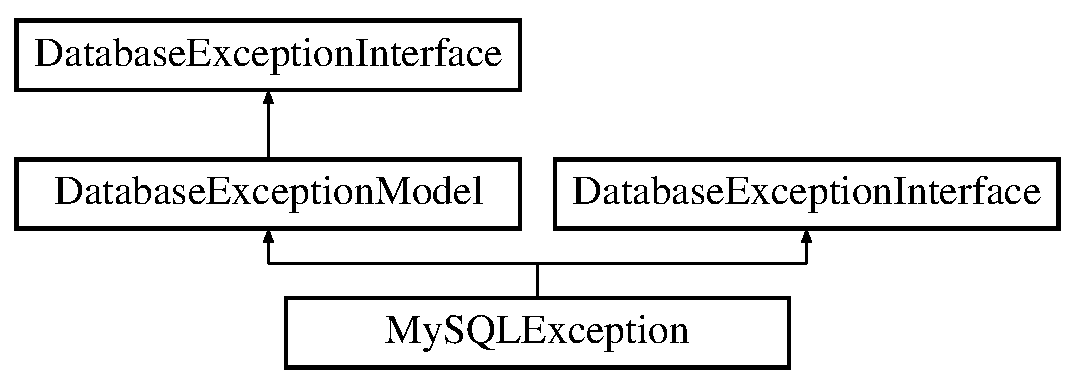
\includegraphics[height=3.000000cm]{class_my_s_q_l_exception}
\end{center}
\end{figure}
\subsection*{Additional Inherited Members}


\subsection{Detailed Description}


Definition at line 3 of file My\+S\+Q\+L\+Exception.\+php.



The documentation for this class was generated from the following file\+:\begin{DoxyCompactItemize}
\item 
src/class/\hyperlink{_my_s_q_l_exception_8php}{My\+S\+Q\+L\+Exception.\+php}\end{DoxyCompactItemize}

\hypertarget{class_postgre_s_q_l_condition}{}\section{Postgre\+S\+Q\+L\+Condition Class Reference}
\label{class_postgre_s_q_l_condition}\index{Postgre\+S\+Q\+L\+Condition@{Postgre\+S\+Q\+L\+Condition}}
Inheritance diagram for Postgre\+S\+Q\+L\+Condition\+:\begin{figure}[H]
\begin{center}
\leavevmode
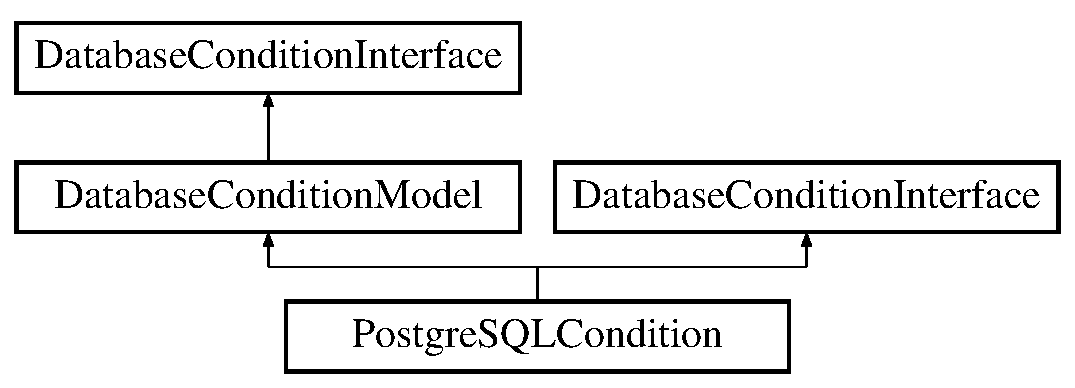
\includegraphics[height=3.000000cm]{class_postgre_s_q_l_condition}
\end{center}
\end{figure}
\subsection*{Additional Inherited Members}


\subsection{Detailed Description}


Definition at line 3 of file Postgre\+S\+Q\+L\+Condition.\+php.



The documentation for this class was generated from the following file\+:\begin{DoxyCompactItemize}
\item 
src/class/\hyperlink{_postgre_s_q_l_condition_8php}{Postgre\+S\+Q\+L\+Condition.\+php}\end{DoxyCompactItemize}

\hypertarget{class_postgre_s_q_l_database}{}\section{Postgre\+S\+Q\+L\+Database Class Reference}
\label{class_postgre_s_q_l_database}\index{Postgre\+S\+Q\+L\+Database@{Postgre\+S\+Q\+L\+Database}}
Inheritance diagram for Postgre\+S\+Q\+L\+Database\+:\begin{figure}[H]
\begin{center}
\leavevmode
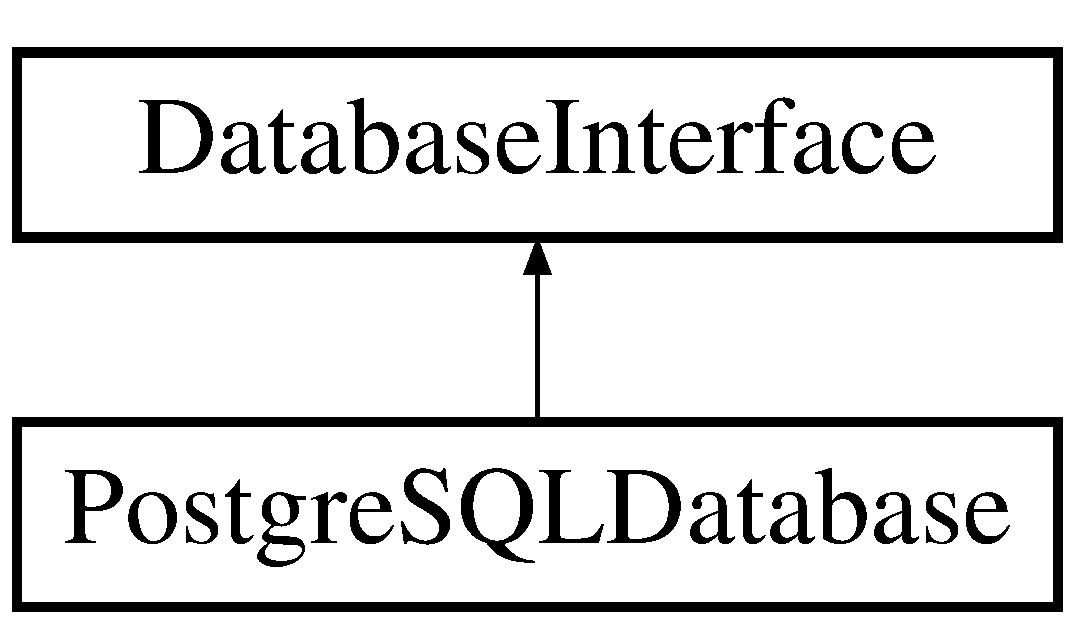
\includegraphics[height=2.000000cm]{class_postgre_s_q_l_database}
\end{center}
\end{figure}
\subsection*{Public Member Functions}
\begin{DoxyCompactItemize}
\item 
\hyperlink{class_postgre_s_q_l_database_a522739237db8d43369172cfe07bf7b85}{\+\_\+\+\_\+construct} (\$name, \$user=null, \$pass=null, \$host= \textquotesingle{}localhost\textquotesingle{}, \$port=null, \$table=null)
\item 
\hyperlink{class_postgre_s_q_l_database_a421831a265621325e1fdd19aace0c758}{\+\_\+\+\_\+destruct} ()
\item 
\hyperlink{class_postgre_s_q_l_database_a9aac7e1475efe923de4e19cc2511f092}{\+\_\+\+\_\+invoke} ()
\item 
\hyperlink{class_postgre_s_q_l_database_a7516ca30af0db3cdbf9a7739b48ce91d}{\+\_\+\+\_\+to\+String} ()
\item 
\hyperlink{class_postgre_s_q_l_database_a42c4cefdb183a7caa3115193a811d893}{column\+Exists} (\$column, \$table=null)
\item 
\hyperlink{class_postgre_s_q_l_database_a5cc0962e790b9ccffd2ca9c77cead320}{get\+Columns} (\$table=null)
\item 
\hyperlink{class_postgre_s_q_l_database_af54c3eed64c3e3dfb06a2541289ff0da}{get\+Default\+Table} ()
\item 
\hyperlink{class_postgre_s_q_l_database_a61b9097ace78236a1a7f9cfd9e9ab01c}{get\+Tables} ()
\item 
\hyperlink{class_postgre_s_q_l_database_a830b5c75df72b32396701bc563fbe3c7}{get\+Type} ()
\item 
\hyperlink{class_postgre_s_q_l_database_ad0aa1804fc79c22b46596db136320017}{has\+Default\+Table} ()
\item 
\hyperlink{class_postgre_s_q_l_database_a8e5626f114925dee9986c8edbfc3ec05}{insert} (\$in, \$table=null)
\item 
\& \hyperlink{class_postgre_s_q_l_database_ae6979f06c8e38dbe758ff53f7395531f}{ref} ()
\item 
\hyperlink{class_postgre_s_q_l_database_a1efc6b974510d4c668660f1abe184182}{select} (\$columns=\mbox{[}\textquotesingle{}$\ast$\textquotesingle{}\mbox{]}, \$conditions=null, \$start=null, \$count=null, \$sort\+By=null, \$sort\+Direction=null, \$table=null)
\item 
\hyperlink{class_postgre_s_q_l_database_ae7cdaa744d52a1eb0103e377023ca528}{table\+Exists} (\$table)
\end{DoxyCompactItemize}
\subsection*{Data Fields}
\begin{DoxyCompactItemize}
\item 
const \hyperlink{class_postgre_s_q_l_database_ac3188f4350978425c488580c5cea8468}{F\+I\+E\+L\+D\+\_\+\+D\+A\+T\+A} = 0
\item 
const \hyperlink{class_postgre_s_q_l_database_acbdf154a35cfc228dd1016e8aa4bd503}{F\+I\+E\+L\+D\+\_\+\+T\+A\+B\+L\+E} = 1
\item 
const \hyperlink{class_postgre_s_q_l_database_a87aad3e89cc6a17f293cf5410b225bbe}{F\+I\+E\+L\+D\+\_\+\+C\+O\+L\+U\+M\+N} = 2
\item 
const \hyperlink{class_postgre_s_q_l_database_a9b1a24ef01d468c146a71b333edb0c17}{K\+E\+Y\+W\+O\+R\+D\+\_\+\+N\+O\+N\+E} = 0
\item 
const \hyperlink{class_postgre_s_q_l_database_ababb5c4af464938f3f0b8f9c4fa183ba}{K\+E\+Y\+W\+O\+R\+D\+\_\+\+A\+L\+L} = 1
\item 
const \hyperlink{class_postgre_s_q_l_database_af3826c676cb54905f393f9d1f7ad48ea}{S\+O\+R\+T\+\_\+\+N\+O\+N\+E} = 0
\item 
const \hyperlink{class_postgre_s_q_l_database_a9517f2622dfc5fbb0cc64feef247eb06}{S\+O\+R\+T\+\_\+\+A\+S\+C} = 1
\item 
const \hyperlink{class_postgre_s_q_l_database_a0e633ab431ae1e5cc483a37cfe73bb09}{S\+O\+R\+T\+\_\+\+D\+E\+S\+C} = 2
\end{DoxyCompactItemize}
\subsection*{Protected Attributes}
\begin{DoxyCompactItemize}
\item 
\hyperlink{class_postgre_s_q_l_database_a49c7011be9c979d9174c52a8b83e5d8e}{\$config}
\item 
\hyperlink{class_postgre_s_q_l_database_a7c7a1968b87fd4d016e364b27b7a3d7d}{\$connector}
\item 
\hyperlink{class_postgre_s_q_l_database_aee271b7ce67fbe00b9976e6c347cbfbf}{\$encoding}
\item 
\hyperlink{class_postgre_s_q_l_database_a711797613cb863ca0756df789c396bf2}{\$host}
\item 
\hyperlink{class_postgre_s_q_l_database_ae19722790c6683980bbf0af8572f26ab}{\$info}
\item 
\hyperlink{class_postgre_s_q_l_database_a6cb6be70a528323568af007db6a3885e}{\$last\+Error}
\item 
\hyperlink{class_postgre_s_q_l_database_a12ff8f78a47e0fa691355a485c2e696a}{\$last\+Stack\+Trace}
\item 
\hyperlink{class_postgre_s_q_l_database_ab2fc40d43824ea3e1ce5d86dee0d763b}{\$name}
\item 
\hyperlink{class_postgre_s_q_l_database_a4269f690c0554ecb1deec21b80f321dc}{\$open}
\item 
\hyperlink{class_postgre_s_q_l_database_aa0787efab4b22e8a212882f3409d4c77}{\$port}
\item 
\hyperlink{class_postgre_s_q_l_database_ae8876a14058f368335baccf35af4a22b}{\$table}
\end{DoxyCompactItemize}


\subsection{Detailed Description}


Definition at line 3 of file Postgre\+S\+Q\+L\+Database.\+php.



\subsection{Constructor \& Destructor Documentation}
\hypertarget{class_postgre_s_q_l_database_a522739237db8d43369172cfe07bf7b85}{}\index{Postgre\+S\+Q\+L\+Database@{Postgre\+S\+Q\+L\+Database}!\+\_\+\+\_\+construct@{\+\_\+\+\_\+construct}}
\index{\+\_\+\+\_\+construct@{\+\_\+\+\_\+construct}!Postgre\+S\+Q\+L\+Database@{Postgre\+S\+Q\+L\+Database}}
\subsubsection[{\+\_\+\+\_\+construct}]{\setlength{\rightskip}{0pt plus 5cm}\+\_\+\+\_\+construct (
\begin{DoxyParamCaption}
\item[{}]{\$name, }
\item[{}]{\$user = {\ttfamily null}, }
\item[{}]{\$pass = {\ttfamily null}, }
\item[{}]{\$host = {\ttfamily \textquotesingle{}localhost\textquotesingle{}}, }
\item[{}]{\$port = {\ttfamily null}, }
\item[{}]{\$table = {\ttfamily null}}
\end{DoxyParamCaption}
)}\label{class_postgre_s_q_l_database_a522739237db8d43369172cfe07bf7b85}
Constructor Method 
\begin{DoxyParams}[1]{Parameters}
int & {\em \$type} & (required) -\/ \\
\hline
string & {\em \$name} & (required) -\/ \\
\hline
string & {\em \$user} & (required for secured) -\/ \\
\hline
string & {\em \$pass} & (required for secured) -\/ \\
\hline
string & {\em \$host} & (required for remote, optional because it defaults to localhost) -\/ \\
\hline
integer & {\em \$port} & (required for remote, optional because it defaults to server type\textquotesingle{}s default port) -\/ \\
\hline
strign & {\em \$table} & (optional) -\/ \\
\hline
\end{DoxyParams}


Definition at line 44 of file Postgre\+S\+Q\+L\+Database.\+php.

\hypertarget{class_postgre_s_q_l_database_a421831a265621325e1fdd19aace0c758}{}\index{Postgre\+S\+Q\+L\+Database@{Postgre\+S\+Q\+L\+Database}!\+\_\+\+\_\+destruct@{\+\_\+\+\_\+destruct}}
\index{\+\_\+\+\_\+destruct@{\+\_\+\+\_\+destruct}!Postgre\+S\+Q\+L\+Database@{Postgre\+S\+Q\+L\+Database}}
\subsubsection[{\+\_\+\+\_\+destruct}]{\setlength{\rightskip}{0pt plus 5cm}\+\_\+\+\_\+destruct (
\begin{DoxyParamCaption}
{}
\end{DoxyParamCaption}
)}\label{class_postgre_s_q_l_database_a421831a265621325e1fdd19aace0c758}
Destructor Method 

Definition at line 262 of file Postgre\+S\+Q\+L\+Database.\+php.



\subsection{Member Function Documentation}
\hypertarget{class_postgre_s_q_l_database_a9aac7e1475efe923de4e19cc2511f092}{}\index{Postgre\+S\+Q\+L\+Database@{Postgre\+S\+Q\+L\+Database}!\+\_\+\+\_\+invoke@{\+\_\+\+\_\+invoke}}
\index{\+\_\+\+\_\+invoke@{\+\_\+\+\_\+invoke}!Postgre\+S\+Q\+L\+Database@{Postgre\+S\+Q\+L\+Database}}
\subsubsection[{\+\_\+\+\_\+invoke}]{\setlength{\rightskip}{0pt plus 5cm}\+\_\+\+\_\+invoke (
\begin{DoxyParamCaption}
{}
\end{DoxyParamCaption}
)}\label{class_postgre_s_q_l_database_a9aac7e1475efe923de4e19cc2511f092}
Invocation Method 

Implements \hyperlink{interface_database_interface_a9aac7e1475efe923de4e19cc2511f092}{Database\+Interface}.



Definition at line 271 of file Postgre\+S\+Q\+L\+Database.\+php.

\hypertarget{class_postgre_s_q_l_database_a7516ca30af0db3cdbf9a7739b48ce91d}{}\index{Postgre\+S\+Q\+L\+Database@{Postgre\+S\+Q\+L\+Database}!\+\_\+\+\_\+to\+String@{\+\_\+\+\_\+to\+String}}
\index{\+\_\+\+\_\+to\+String@{\+\_\+\+\_\+to\+String}!Postgre\+S\+Q\+L\+Database@{Postgre\+S\+Q\+L\+Database}}
\subsubsection[{\+\_\+\+\_\+to\+String}]{\setlength{\rightskip}{0pt plus 5cm}\+\_\+\+\_\+to\+String (
\begin{DoxyParamCaption}
{}
\end{DoxyParamCaption}
)}\label{class_postgre_s_q_l_database_a7516ca30af0db3cdbf9a7739b48ce91d}
String Conversion Method 

Implements \hyperlink{interface_database_interface_a7516ca30af0db3cdbf9a7739b48ce91d}{Database\+Interface}.



Definition at line 280 of file Postgre\+S\+Q\+L\+Database.\+php.

\hypertarget{class_postgre_s_q_l_database_a42c4cefdb183a7caa3115193a811d893}{}\index{Postgre\+S\+Q\+L\+Database@{Postgre\+S\+Q\+L\+Database}!column\+Exists@{column\+Exists}}
\index{column\+Exists@{column\+Exists}!Postgre\+S\+Q\+L\+Database@{Postgre\+S\+Q\+L\+Database}}
\subsubsection[{column\+Exists}]{\setlength{\rightskip}{0pt plus 5cm}column\+Exists (
\begin{DoxyParamCaption}
\item[{}]{\$column, }
\item[{}]{\$table = {\ttfamily null}}
\end{DoxyParamCaption}
)}\label{class_postgre_s_q_l_database_a42c4cefdb183a7caa3115193a811d893}


Definition at line 286 of file Postgre\+S\+Q\+L\+Database.\+php.

\hypertarget{class_postgre_s_q_l_database_a5cc0962e790b9ccffd2ca9c77cead320}{}\index{Postgre\+S\+Q\+L\+Database@{Postgre\+S\+Q\+L\+Database}!get\+Columns@{get\+Columns}}
\index{get\+Columns@{get\+Columns}!Postgre\+S\+Q\+L\+Database@{Postgre\+S\+Q\+L\+Database}}
\subsubsection[{get\+Columns}]{\setlength{\rightskip}{0pt plus 5cm}get\+Columns (
\begin{DoxyParamCaption}
\item[{}]{\$table = {\ttfamily null}}
\end{DoxyParamCaption}
)}\label{class_postgre_s_q_l_database_a5cc0962e790b9ccffd2ca9c77cead320}
Database-\/$>$\hyperlink{interface_database_interface_a6287262cb9628d7a89d8fc16dcb51177}{get\+Columns()} Method


\begin{DoxyParams}[1]{Parameters}
string & {\em \$table} & (optional) -\/ name of table, unless table defined by constructor \\
\hline
\end{DoxyParams}
\begin{DoxyReturn}{Returns}
array -\/ array of columns in the table 
\end{DoxyReturn}


Definition at line 377 of file Postgre\+S\+Q\+L\+Database.\+php.

\hypertarget{class_postgre_s_q_l_database_af54c3eed64c3e3dfb06a2541289ff0da}{}\index{Postgre\+S\+Q\+L\+Database@{Postgre\+S\+Q\+L\+Database}!get\+Default\+Table@{get\+Default\+Table}}
\index{get\+Default\+Table@{get\+Default\+Table}!Postgre\+S\+Q\+L\+Database@{Postgre\+S\+Q\+L\+Database}}
\subsubsection[{get\+Default\+Table}]{\setlength{\rightskip}{0pt plus 5cm}get\+Default\+Table (
\begin{DoxyParamCaption}
{}
\end{DoxyParamCaption}
)}\label{class_postgre_s_q_l_database_af54c3eed64c3e3dfb06a2541289ff0da}


Implements \hyperlink{interface_database_interface_af54c3eed64c3e3dfb06a2541289ff0da}{Database\+Interface}.



Definition at line 426 of file Postgre\+S\+Q\+L\+Database.\+php.

\hypertarget{class_postgre_s_q_l_database_a61b9097ace78236a1a7f9cfd9e9ab01c}{}\index{Postgre\+S\+Q\+L\+Database@{Postgre\+S\+Q\+L\+Database}!get\+Tables@{get\+Tables}}
\index{get\+Tables@{get\+Tables}!Postgre\+S\+Q\+L\+Database@{Postgre\+S\+Q\+L\+Database}}
\subsubsection[{get\+Tables}]{\setlength{\rightskip}{0pt plus 5cm}get\+Tables (
\begin{DoxyParamCaption}
{}
\end{DoxyParamCaption}
)}\label{class_postgre_s_q_l_database_a61b9097ace78236a1a7f9cfd9e9ab01c}


Implements \hyperlink{interface_database_interface_a61b9097ace78236a1a7f9cfd9e9ab01c}{Database\+Interface}.



Definition at line 432 of file Postgre\+S\+Q\+L\+Database.\+php.

\hypertarget{class_postgre_s_q_l_database_a830b5c75df72b32396701bc563fbe3c7}{}\index{Postgre\+S\+Q\+L\+Database@{Postgre\+S\+Q\+L\+Database}!get\+Type@{get\+Type}}
\index{get\+Type@{get\+Type}!Postgre\+S\+Q\+L\+Database@{Postgre\+S\+Q\+L\+Database}}
\subsubsection[{get\+Type}]{\setlength{\rightskip}{0pt plus 5cm}get\+Type (
\begin{DoxyParamCaption}
{}
\end{DoxyParamCaption}
)}\label{class_postgre_s_q_l_database_a830b5c75df72b32396701bc563fbe3c7}
Database-\/$>$\hyperlink{class_postgre_s_q_l_database_a830b5c75df72b32396701bc563fbe3c7}{get\+Type()} Getter Method \begin{DoxyReturn}{Returns}
string \$this-\/$>$type 
\end{DoxyReturn}


Definition at line 465 of file Postgre\+S\+Q\+L\+Database.\+php.

\hypertarget{class_postgre_s_q_l_database_ad0aa1804fc79c22b46596db136320017}{}\index{Postgre\+S\+Q\+L\+Database@{Postgre\+S\+Q\+L\+Database}!has\+Default\+Table@{has\+Default\+Table}}
\index{has\+Default\+Table@{has\+Default\+Table}!Postgre\+S\+Q\+L\+Database@{Postgre\+S\+Q\+L\+Database}}
\subsubsection[{has\+Default\+Table}]{\setlength{\rightskip}{0pt plus 5cm}has\+Default\+Table (
\begin{DoxyParamCaption}
{}
\end{DoxyParamCaption}
)}\label{class_postgre_s_q_l_database_ad0aa1804fc79c22b46596db136320017}


Implements \hyperlink{interface_database_interface_ad0aa1804fc79c22b46596db136320017}{Database\+Interface}.



Definition at line 471 of file Postgre\+S\+Q\+L\+Database.\+php.

\hypertarget{class_postgre_s_q_l_database_a8e5626f114925dee9986c8edbfc3ec05}{}\index{Postgre\+S\+Q\+L\+Database@{Postgre\+S\+Q\+L\+Database}!insert@{insert}}
\index{insert@{insert}!Postgre\+S\+Q\+L\+Database@{Postgre\+S\+Q\+L\+Database}}
\subsubsection[{insert}]{\setlength{\rightskip}{0pt plus 5cm}insert (
\begin{DoxyParamCaption}
\item[{}]{\$in, }
\item[{}]{\$table = {\ttfamily null}}
\end{DoxyParamCaption}
)}\label{class_postgre_s_q_l_database_a8e5626f114925dee9986c8edbfc3ec05}
Database-\/$>$\hyperlink{class_postgre_s_q_l_database_a8e5626f114925dee9986c8edbfc3ec05}{insert()} Method


\begin{DoxyParams}[1]{Parameters}
array & {\em \$in} & (required) -\/ associative array of input to be inserted, keys being the name of columns \\
\hline
string & {\em \$table} & (optional if defined in constructor) -\/ table to use \\
\hline
\end{DoxyParams}
\begin{DoxyReturn}{Returns}
\hyperlink{class_database}{Database} -\/ reference to self 
\end{DoxyReturn}


Implements \hyperlink{interface_database_interface_a8e5626f114925dee9986c8edbfc3ec05}{Database\+Interface}.



Definition at line 488 of file Postgre\+S\+Q\+L\+Database.\+php.

\hypertarget{class_postgre_s_q_l_database_ae6979f06c8e38dbe758ff53f7395531f}{}\index{Postgre\+S\+Q\+L\+Database@{Postgre\+S\+Q\+L\+Database}!ref@{ref}}
\index{ref@{ref}!Postgre\+S\+Q\+L\+Database@{Postgre\+S\+Q\+L\+Database}}
\subsubsection[{ref}]{\setlength{\rightskip}{0pt plus 5cm}\& ref (
\begin{DoxyParamCaption}
{}
\end{DoxyParamCaption}
)}\label{class_postgre_s_q_l_database_ae6979f06c8e38dbe758ff53f7395531f}
Self Reference Method \begin{DoxyReturn}{Returns}
\hyperlink{class_database}{Database} 
\end{DoxyReturn}


Definition at line 624 of file Postgre\+S\+Q\+L\+Database.\+php.

\hypertarget{class_postgre_s_q_l_database_a1efc6b974510d4c668660f1abe184182}{}\index{Postgre\+S\+Q\+L\+Database@{Postgre\+S\+Q\+L\+Database}!select@{select}}
\index{select@{select}!Postgre\+S\+Q\+L\+Database@{Postgre\+S\+Q\+L\+Database}}
\subsubsection[{select}]{\setlength{\rightskip}{0pt plus 5cm}select (
\begin{DoxyParamCaption}
\item[{}]{\$columns = {\ttfamily \mbox{[}\textquotesingle{}$\ast$\textquotesingle{}\mbox{]}}, }
\item[{}]{\$conditions = {\ttfamily null}, }
\item[{}]{\$start = {\ttfamily null}, }
\item[{}]{\$count = {\ttfamily null}, }
\item[{}]{\$sort\+By = {\ttfamily null}, }
\item[{}]{\$sort\+Direction = {\ttfamily null}, }
\item[{}]{\$table = {\ttfamily null}}
\end{DoxyParamCaption}
)}\label{class_postgre_s_q_l_database_a1efc6b974510d4c668660f1abe184182}
Database-\/$>$\hyperlink{class_postgre_s_q_l_database_a1efc6b974510d4c668660f1abe184182}{select()} Method


\begin{DoxyParams}[1]{Parameters}
array | string & {\em \$columns} & (optional) -\/ columns to return. if left empty/null, will default to all columns ($\ast$) \\
\hline
Database\+Condition | array | string & {\em \$conditions} & (optional) -\/ conditions to lookup. If left empty/null, will default to no conditions. \\
\hline
int & {\em \$start} & (optional) -\/ starting index from which to begin selecting. If left empty, defaults to 0. \\
\hline
int & {\em \$count} & (optional) -\/ maximum number of results to return. If left empty, defaults to no limit. \\
\hline
string & {\em \$sort\+By} & (optional) -\/ column with which to sort the table. If left empty, defaults to the first column in the table. \\
\hline
int & {\em \$sort\+Direction} & (optional -\/ (uses flags) direction to sort the table. If left empty, defaults to none. Options are S\+O\+R\+T\+\_\+\+N\+O\+N\+E, S\+O\+R\+T\+\_\+\+A\+S\+C, S\+O\+R\+T\+\_\+\+D\+E\+S\+C \\
\hline
string & {\em \$table} & (optional if table set in constructor) -\/ table from which to select. return array -\/ results of the select query as an associative array. \\
\hline
\end{DoxyParams}


Implements \hyperlink{interface_database_interface_a1efc6b974510d4c668660f1abe184182}{Database\+Interface}.



Definition at line 642 of file Postgre\+S\+Q\+L\+Database.\+php.

\hypertarget{class_postgre_s_q_l_database_ae7cdaa744d52a1eb0103e377023ca528}{}\index{Postgre\+S\+Q\+L\+Database@{Postgre\+S\+Q\+L\+Database}!table\+Exists@{table\+Exists}}
\index{table\+Exists@{table\+Exists}!Postgre\+S\+Q\+L\+Database@{Postgre\+S\+Q\+L\+Database}}
\subsubsection[{table\+Exists}]{\setlength{\rightskip}{0pt plus 5cm}table\+Exists (
\begin{DoxyParamCaption}
\item[{}]{\$table}
\end{DoxyParamCaption}
)}\label{class_postgre_s_q_l_database_ae7cdaa744d52a1eb0103e377023ca528}


Implements \hyperlink{interface_database_interface_ae7cdaa744d52a1eb0103e377023ca528}{Database\+Interface}.



Definition at line 899 of file Postgre\+S\+Q\+L\+Database.\+php.



\subsection{Field Documentation}
\hypertarget{class_postgre_s_q_l_database_a49c7011be9c979d9174c52a8b83e5d8e}{}\index{Postgre\+S\+Q\+L\+Database@{Postgre\+S\+Q\+L\+Database}!\$config@{\$config}}
\index{\$config@{\$config}!Postgre\+S\+Q\+L\+Database@{Postgre\+S\+Q\+L\+Database}}
\subsubsection[{\$config}]{\setlength{\rightskip}{0pt plus 5cm}\$config\hspace{0.3cm}{\ttfamily [protected]}}\label{class_postgre_s_q_l_database_a49c7011be9c979d9174c52a8b83e5d8e}
{\bfseries Initial value\+:}
\begin{DoxyCode}
= [
        \textcolor{stringliteral}{'defaultPort'} => 5432
\end{DoxyCode}


Definition at line 7 of file Postgre\+S\+Q\+L\+Database.\+php.

\hypertarget{class_postgre_s_q_l_database_a7c7a1968b87fd4d016e364b27b7a3d7d}{}\index{Postgre\+S\+Q\+L\+Database@{Postgre\+S\+Q\+L\+Database}!\$connector@{\$connector}}
\index{\$connector@{\$connector}!Postgre\+S\+Q\+L\+Database@{Postgre\+S\+Q\+L\+Database}}
\subsubsection[{\$connector}]{\setlength{\rightskip}{0pt plus 5cm}\$connector\hspace{0.3cm}{\ttfamily [protected]}}\label{class_postgre_s_q_l_database_a7c7a1968b87fd4d016e364b27b7a3d7d}


Definition at line 7 of file Postgre\+S\+Q\+L\+Database.\+php.

\hypertarget{class_postgre_s_q_l_database_aee271b7ce67fbe00b9976e6c347cbfbf}{}\index{Postgre\+S\+Q\+L\+Database@{Postgre\+S\+Q\+L\+Database}!\$encoding@{\$encoding}}
\index{\$encoding@{\$encoding}!Postgre\+S\+Q\+L\+Database@{Postgre\+S\+Q\+L\+Database}}
\subsubsection[{\$encoding}]{\setlength{\rightskip}{0pt plus 5cm}\$encoding\hspace{0.3cm}{\ttfamily [protected]}}\label{class_postgre_s_q_l_database_aee271b7ce67fbe00b9976e6c347cbfbf}


Definition at line 11 of file Postgre\+S\+Q\+L\+Database.\+php.

\hypertarget{class_postgre_s_q_l_database_a711797613cb863ca0756df789c396bf2}{}\index{Postgre\+S\+Q\+L\+Database@{Postgre\+S\+Q\+L\+Database}!\$host@{\$host}}
\index{\$host@{\$host}!Postgre\+S\+Q\+L\+Database@{Postgre\+S\+Q\+L\+Database}}
\subsubsection[{\$host}]{\setlength{\rightskip}{0pt plus 5cm}\$host\hspace{0.3cm}{\ttfamily [protected]}}\label{class_postgre_s_q_l_database_a711797613cb863ca0756df789c396bf2}


Definition at line 12 of file Postgre\+S\+Q\+L\+Database.\+php.

\hypertarget{class_postgre_s_q_l_database_ae19722790c6683980bbf0af8572f26ab}{}\index{Postgre\+S\+Q\+L\+Database@{Postgre\+S\+Q\+L\+Database}!\$info@{\$info}}
\index{\$info@{\$info}!Postgre\+S\+Q\+L\+Database@{Postgre\+S\+Q\+L\+Database}}
\subsubsection[{\$info}]{\setlength{\rightskip}{0pt plus 5cm}\$info\hspace{0.3cm}{\ttfamily [protected]}}\label{class_postgre_s_q_l_database_ae19722790c6683980bbf0af8572f26ab}


Definition at line 13 of file Postgre\+S\+Q\+L\+Database.\+php.

\hypertarget{class_postgre_s_q_l_database_a6cb6be70a528323568af007db6a3885e}{}\index{Postgre\+S\+Q\+L\+Database@{Postgre\+S\+Q\+L\+Database}!\$last\+Error@{\$last\+Error}}
\index{\$last\+Error@{\$last\+Error}!Postgre\+S\+Q\+L\+Database@{Postgre\+S\+Q\+L\+Database}}
\subsubsection[{\$last\+Error}]{\setlength{\rightskip}{0pt plus 5cm}\$last\+Error\hspace{0.3cm}{\ttfamily [protected]}}\label{class_postgre_s_q_l_database_a6cb6be70a528323568af007db6a3885e}


Definition at line 14 of file Postgre\+S\+Q\+L\+Database.\+php.

\hypertarget{class_postgre_s_q_l_database_a12ff8f78a47e0fa691355a485c2e696a}{}\index{Postgre\+S\+Q\+L\+Database@{Postgre\+S\+Q\+L\+Database}!\$last\+Stack\+Trace@{\$last\+Stack\+Trace}}
\index{\$last\+Stack\+Trace@{\$last\+Stack\+Trace}!Postgre\+S\+Q\+L\+Database@{Postgre\+S\+Q\+L\+Database}}
\subsubsection[{\$last\+Stack\+Trace}]{\setlength{\rightskip}{0pt plus 5cm}\$last\+Stack\+Trace\hspace{0.3cm}{\ttfamily [protected]}}\label{class_postgre_s_q_l_database_a12ff8f78a47e0fa691355a485c2e696a}


Definition at line 15 of file Postgre\+S\+Q\+L\+Database.\+php.

\hypertarget{class_postgre_s_q_l_database_ab2fc40d43824ea3e1ce5d86dee0d763b}{}\index{Postgre\+S\+Q\+L\+Database@{Postgre\+S\+Q\+L\+Database}!\$name@{\$name}}
\index{\$name@{\$name}!Postgre\+S\+Q\+L\+Database@{Postgre\+S\+Q\+L\+Database}}
\subsubsection[{\$name}]{\setlength{\rightskip}{0pt plus 5cm}\$name\hspace{0.3cm}{\ttfamily [protected]}}\label{class_postgre_s_q_l_database_ab2fc40d43824ea3e1ce5d86dee0d763b}


Definition at line 16 of file Postgre\+S\+Q\+L\+Database.\+php.

\hypertarget{class_postgre_s_q_l_database_a4269f690c0554ecb1deec21b80f321dc}{}\index{Postgre\+S\+Q\+L\+Database@{Postgre\+S\+Q\+L\+Database}!\$open@{\$open}}
\index{\$open@{\$open}!Postgre\+S\+Q\+L\+Database@{Postgre\+S\+Q\+L\+Database}}
\subsubsection[{\$open}]{\setlength{\rightskip}{0pt plus 5cm}\$open\hspace{0.3cm}{\ttfamily [protected]}}\label{class_postgre_s_q_l_database_a4269f690c0554ecb1deec21b80f321dc}


Definition at line 17 of file Postgre\+S\+Q\+L\+Database.\+php.

\hypertarget{class_postgre_s_q_l_database_aa0787efab4b22e8a212882f3409d4c77}{}\index{Postgre\+S\+Q\+L\+Database@{Postgre\+S\+Q\+L\+Database}!\$port@{\$port}}
\index{\$port@{\$port}!Postgre\+S\+Q\+L\+Database@{Postgre\+S\+Q\+L\+Database}}
\subsubsection[{\$port}]{\setlength{\rightskip}{0pt plus 5cm}\$port\hspace{0.3cm}{\ttfamily [protected]}}\label{class_postgre_s_q_l_database_aa0787efab4b22e8a212882f3409d4c77}


Definition at line 18 of file Postgre\+S\+Q\+L\+Database.\+php.

\hypertarget{class_postgre_s_q_l_database_ae8876a14058f368335baccf35af4a22b}{}\index{Postgre\+S\+Q\+L\+Database@{Postgre\+S\+Q\+L\+Database}!\$table@{\$table}}
\index{\$table@{\$table}!Postgre\+S\+Q\+L\+Database@{Postgre\+S\+Q\+L\+Database}}
\subsubsection[{\$table}]{\setlength{\rightskip}{0pt plus 5cm}\$table\hspace{0.3cm}{\ttfamily [protected]}}\label{class_postgre_s_q_l_database_ae8876a14058f368335baccf35af4a22b}


Definition at line 19 of file Postgre\+S\+Q\+L\+Database.\+php.

\hypertarget{class_postgre_s_q_l_database_a87aad3e89cc6a17f293cf5410b225bbe}{}\index{Postgre\+S\+Q\+L\+Database@{Postgre\+S\+Q\+L\+Database}!F\+I\+E\+L\+D\+\_\+\+C\+O\+L\+U\+M\+N@{F\+I\+E\+L\+D\+\_\+\+C\+O\+L\+U\+M\+N}}
\index{F\+I\+E\+L\+D\+\_\+\+C\+O\+L\+U\+M\+N@{F\+I\+E\+L\+D\+\_\+\+C\+O\+L\+U\+M\+N}!Postgre\+S\+Q\+L\+Database@{Postgre\+S\+Q\+L\+Database}}
\subsubsection[{F\+I\+E\+L\+D\+\_\+\+C\+O\+L\+U\+M\+N}]{\setlength{\rightskip}{0pt plus 5cm}const F\+I\+E\+L\+D\+\_\+\+C\+O\+L\+U\+M\+N = 2}\label{class_postgre_s_q_l_database_a87aad3e89cc6a17f293cf5410b225bbe}


Definition at line 25 of file Postgre\+S\+Q\+L\+Database.\+php.

\hypertarget{class_postgre_s_q_l_database_ac3188f4350978425c488580c5cea8468}{}\index{Postgre\+S\+Q\+L\+Database@{Postgre\+S\+Q\+L\+Database}!F\+I\+E\+L\+D\+\_\+\+D\+A\+T\+A@{F\+I\+E\+L\+D\+\_\+\+D\+A\+T\+A}}
\index{F\+I\+E\+L\+D\+\_\+\+D\+A\+T\+A@{F\+I\+E\+L\+D\+\_\+\+D\+A\+T\+A}!Postgre\+S\+Q\+L\+Database@{Postgre\+S\+Q\+L\+Database}}
\subsubsection[{F\+I\+E\+L\+D\+\_\+\+D\+A\+T\+A}]{\setlength{\rightskip}{0pt plus 5cm}const F\+I\+E\+L\+D\+\_\+\+D\+A\+T\+A = 0}\label{class_postgre_s_q_l_database_ac3188f4350978425c488580c5cea8468}


Definition at line 23 of file Postgre\+S\+Q\+L\+Database.\+php.

\hypertarget{class_postgre_s_q_l_database_acbdf154a35cfc228dd1016e8aa4bd503}{}\index{Postgre\+S\+Q\+L\+Database@{Postgre\+S\+Q\+L\+Database}!F\+I\+E\+L\+D\+\_\+\+T\+A\+B\+L\+E@{F\+I\+E\+L\+D\+\_\+\+T\+A\+B\+L\+E}}
\index{F\+I\+E\+L\+D\+\_\+\+T\+A\+B\+L\+E@{F\+I\+E\+L\+D\+\_\+\+T\+A\+B\+L\+E}!Postgre\+S\+Q\+L\+Database@{Postgre\+S\+Q\+L\+Database}}
\subsubsection[{F\+I\+E\+L\+D\+\_\+\+T\+A\+B\+L\+E}]{\setlength{\rightskip}{0pt plus 5cm}const F\+I\+E\+L\+D\+\_\+\+T\+A\+B\+L\+E = 1}\label{class_postgre_s_q_l_database_acbdf154a35cfc228dd1016e8aa4bd503}


Definition at line 24 of file Postgre\+S\+Q\+L\+Database.\+php.

\hypertarget{class_postgre_s_q_l_database_ababb5c4af464938f3f0b8f9c4fa183ba}{}\index{Postgre\+S\+Q\+L\+Database@{Postgre\+S\+Q\+L\+Database}!K\+E\+Y\+W\+O\+R\+D\+\_\+\+A\+L\+L@{K\+E\+Y\+W\+O\+R\+D\+\_\+\+A\+L\+L}}
\index{K\+E\+Y\+W\+O\+R\+D\+\_\+\+A\+L\+L@{K\+E\+Y\+W\+O\+R\+D\+\_\+\+A\+L\+L}!Postgre\+S\+Q\+L\+Database@{Postgre\+S\+Q\+L\+Database}}
\subsubsection[{K\+E\+Y\+W\+O\+R\+D\+\_\+\+A\+L\+L}]{\setlength{\rightskip}{0pt plus 5cm}const K\+E\+Y\+W\+O\+R\+D\+\_\+\+A\+L\+L = 1}\label{class_postgre_s_q_l_database_ababb5c4af464938f3f0b8f9c4fa183ba}


Definition at line 28 of file Postgre\+S\+Q\+L\+Database.\+php.

\hypertarget{class_postgre_s_q_l_database_a9b1a24ef01d468c146a71b333edb0c17}{}\index{Postgre\+S\+Q\+L\+Database@{Postgre\+S\+Q\+L\+Database}!K\+E\+Y\+W\+O\+R\+D\+\_\+\+N\+O\+N\+E@{K\+E\+Y\+W\+O\+R\+D\+\_\+\+N\+O\+N\+E}}
\index{K\+E\+Y\+W\+O\+R\+D\+\_\+\+N\+O\+N\+E@{K\+E\+Y\+W\+O\+R\+D\+\_\+\+N\+O\+N\+E}!Postgre\+S\+Q\+L\+Database@{Postgre\+S\+Q\+L\+Database}}
\subsubsection[{K\+E\+Y\+W\+O\+R\+D\+\_\+\+N\+O\+N\+E}]{\setlength{\rightskip}{0pt plus 5cm}const K\+E\+Y\+W\+O\+R\+D\+\_\+\+N\+O\+N\+E = 0}\label{class_postgre_s_q_l_database_a9b1a24ef01d468c146a71b333edb0c17}


Definition at line 27 of file Postgre\+S\+Q\+L\+Database.\+php.

\hypertarget{class_postgre_s_q_l_database_a9517f2622dfc5fbb0cc64feef247eb06}{}\index{Postgre\+S\+Q\+L\+Database@{Postgre\+S\+Q\+L\+Database}!S\+O\+R\+T\+\_\+\+A\+S\+C@{S\+O\+R\+T\+\_\+\+A\+S\+C}}
\index{S\+O\+R\+T\+\_\+\+A\+S\+C@{S\+O\+R\+T\+\_\+\+A\+S\+C}!Postgre\+S\+Q\+L\+Database@{Postgre\+S\+Q\+L\+Database}}
\subsubsection[{S\+O\+R\+T\+\_\+\+A\+S\+C}]{\setlength{\rightskip}{0pt plus 5cm}const S\+O\+R\+T\+\_\+\+A\+S\+C = 1}\label{class_postgre_s_q_l_database_a9517f2622dfc5fbb0cc64feef247eb06}


Definition at line 31 of file Postgre\+S\+Q\+L\+Database.\+php.

\hypertarget{class_postgre_s_q_l_database_a0e633ab431ae1e5cc483a37cfe73bb09}{}\index{Postgre\+S\+Q\+L\+Database@{Postgre\+S\+Q\+L\+Database}!S\+O\+R\+T\+\_\+\+D\+E\+S\+C@{S\+O\+R\+T\+\_\+\+D\+E\+S\+C}}
\index{S\+O\+R\+T\+\_\+\+D\+E\+S\+C@{S\+O\+R\+T\+\_\+\+D\+E\+S\+C}!Postgre\+S\+Q\+L\+Database@{Postgre\+S\+Q\+L\+Database}}
\subsubsection[{S\+O\+R\+T\+\_\+\+D\+E\+S\+C}]{\setlength{\rightskip}{0pt plus 5cm}const S\+O\+R\+T\+\_\+\+D\+E\+S\+C = 2}\label{class_postgre_s_q_l_database_a0e633ab431ae1e5cc483a37cfe73bb09}


Definition at line 32 of file Postgre\+S\+Q\+L\+Database.\+php.

\hypertarget{class_postgre_s_q_l_database_af3826c676cb54905f393f9d1f7ad48ea}{}\index{Postgre\+S\+Q\+L\+Database@{Postgre\+S\+Q\+L\+Database}!S\+O\+R\+T\+\_\+\+N\+O\+N\+E@{S\+O\+R\+T\+\_\+\+N\+O\+N\+E}}
\index{S\+O\+R\+T\+\_\+\+N\+O\+N\+E@{S\+O\+R\+T\+\_\+\+N\+O\+N\+E}!Postgre\+S\+Q\+L\+Database@{Postgre\+S\+Q\+L\+Database}}
\subsubsection[{S\+O\+R\+T\+\_\+\+N\+O\+N\+E}]{\setlength{\rightskip}{0pt plus 5cm}const S\+O\+R\+T\+\_\+\+N\+O\+N\+E = 0}\label{class_postgre_s_q_l_database_af3826c676cb54905f393f9d1f7ad48ea}


Definition at line 30 of file Postgre\+S\+Q\+L\+Database.\+php.



The documentation for this class was generated from the following file\+:\begin{DoxyCompactItemize}
\item 
src/class/\hyperlink{_postgre_s_q_l_database_8php}{Postgre\+S\+Q\+L\+Database.\+php}\end{DoxyCompactItemize}

\hypertarget{class_postgre_s_q_l_exception}{}\section{Postgre\+S\+Q\+L\+Exception Class Reference}
\label{class_postgre_s_q_l_exception}\index{Postgre\+S\+Q\+L\+Exception@{Postgre\+S\+Q\+L\+Exception}}
Inheritance diagram for Postgre\+S\+Q\+L\+Exception\+:\begin{figure}[H]
\begin{center}
\leavevmode
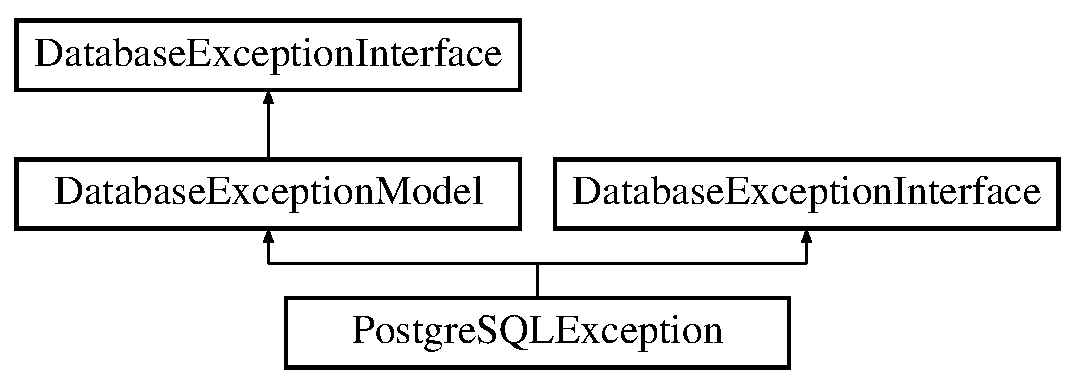
\includegraphics[height=3.000000cm]{class_postgre_s_q_l_exception}
\end{center}
\end{figure}
\subsection*{Additional Inherited Members}


\subsection{Detailed Description}


Definition at line 3 of file Postgre\+S\+Q\+L\+Exception.\+php.



The documentation for this class was generated from the following file\+:\begin{DoxyCompactItemize}
\item 
src/class/\hyperlink{_postgre_s_q_l_exception_8php}{Postgre\+S\+Q\+L\+Exception.\+php}\end{DoxyCompactItemize}

\hypertarget{class_s_q_lite_condition}{}\section{S\+Q\+Lite\+Condition Class Reference}
\label{class_s_q_lite_condition}\index{S\+Q\+Lite\+Condition@{S\+Q\+Lite\+Condition}}
Inheritance diagram for S\+Q\+Lite\+Condition\+:\begin{figure}[H]
\begin{center}
\leavevmode
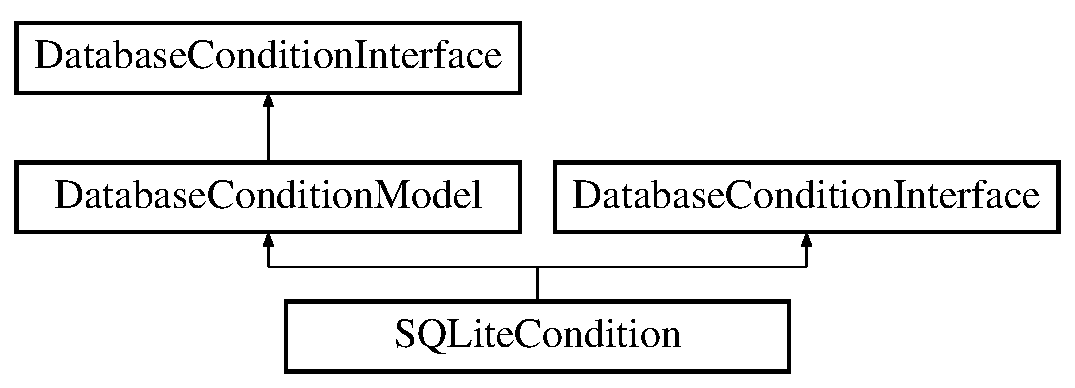
\includegraphics[height=3.000000cm]{class_s_q_lite_condition}
\end{center}
\end{figure}
\subsection*{Additional Inherited Members}


\subsection{Detailed Description}


Definition at line 3 of file S\+Q\+Lite\+Condition.\+php.



The documentation for this class was generated from the following file\+:\begin{DoxyCompactItemize}
\item 
src/class/\hyperlink{_s_q_lite_condition_8php}{S\+Q\+Lite\+Condition.\+php}\end{DoxyCompactItemize}

\hypertarget{class_s_q_lite_database}{}\section{S\+Q\+Lite\+Database Class Reference}
\label{class_s_q_lite_database}\index{S\+Q\+Lite\+Database@{S\+Q\+Lite\+Database}}
Inheritance diagram for S\+Q\+Lite\+Database\+:\begin{figure}[H]
\begin{center}
\leavevmode
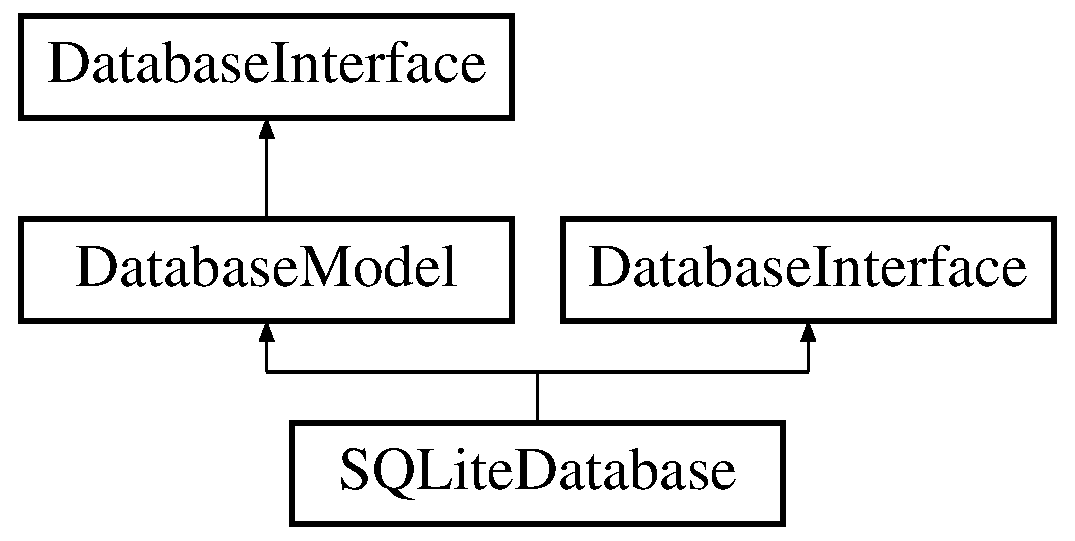
\includegraphics[height=2.000000cm]{class_s_q_lite_database}
\end{center}
\end{figure}
\subsection*{Public Member Functions}
\begin{DoxyCompactItemize}
\item 
\hyperlink{class_s_q_lite_database_a98c33e722c2aeac0d41ff40cfb705f5e}{\+\_\+\+\_\+construct} (\$name, \$table=null)
\item 
\hyperlink{class_s_q_lite_database_a421831a265621325e1fdd19aace0c758}{\+\_\+\+\_\+destruct} ()
\item 
\hyperlink{class_s_q_lite_database_a9aac7e1475efe923de4e19cc2511f092}{\+\_\+\+\_\+invoke} ()
\item 
\hyperlink{class_s_q_lite_database_a7516ca30af0db3cdbf9a7739b48ce91d}{\+\_\+\+\_\+to\+String} ()
\item 
\hyperlink{class_s_q_lite_database_a42c4cefdb183a7caa3115193a811d893}{column\+Exists} (\$column, \$table=null)
\item 
\hyperlink{class_s_q_lite_database_a5cc0962e790b9ccffd2ca9c77cead320}{get\+Columns} (\$table=null)
\item 
\hyperlink{class_s_q_lite_database_af54c3eed64c3e3dfb06a2541289ff0da}{get\+Default\+Table} ()
\item 
\hyperlink{class_s_q_lite_database_a61b9097ace78236a1a7f9cfd9e9ab01c}{get\+Tables} ()
\item 
\hyperlink{class_s_q_lite_database_a830b5c75df72b32396701bc563fbe3c7}{get\+Type} ()
\item 
\hyperlink{class_s_q_lite_database_ad0aa1804fc79c22b46596db136320017}{has\+Default\+Table} ()
\item 
\hyperlink{class_s_q_lite_database_a8e5626f114925dee9986c8edbfc3ec05}{insert} (\$in, \$table=null)
\item 
\& \hyperlink{class_s_q_lite_database_ae6979f06c8e38dbe758ff53f7395531f}{ref} ()
\item 
\hyperlink{class_s_q_lite_database_a1efc6b974510d4c668660f1abe184182}{select} (\$columns=\mbox{[}\textquotesingle{}$\ast$\textquotesingle{}\mbox{]}, \$conditions=null, \$start=null, \$count=null, \$sort\+By=null, \$sort\+Direction=null, \$table=null)
\item 
\hyperlink{class_s_q_lite_database_ae7cdaa744d52a1eb0103e377023ca528}{table\+Exists} (\$table)
\end{DoxyCompactItemize}
\subsection*{Data Fields}
\begin{DoxyCompactItemize}
\item 
const \hyperlink{class_s_q_lite_database_ac3188f4350978425c488580c5cea8468}{F\+I\+E\+L\+D\+\_\+\+D\+A\+T\+A} = 0
\item 
const \hyperlink{class_s_q_lite_database_acbdf154a35cfc228dd1016e8aa4bd503}{F\+I\+E\+L\+D\+\_\+\+T\+A\+B\+L\+E} = 1
\item 
const \hyperlink{class_s_q_lite_database_a87aad3e89cc6a17f293cf5410b225bbe}{F\+I\+E\+L\+D\+\_\+\+C\+O\+L\+U\+M\+N} = 2
\item 
const \hyperlink{class_s_q_lite_database_a9b1a24ef01d468c146a71b333edb0c17}{K\+E\+Y\+W\+O\+R\+D\+\_\+\+N\+O\+N\+E} = 0
\item 
const \hyperlink{class_s_q_lite_database_ababb5c4af464938f3f0b8f9c4fa183ba}{K\+E\+Y\+W\+O\+R\+D\+\_\+\+A\+L\+L} = 1
\item 
const \hyperlink{class_s_q_lite_database_af3826c676cb54905f393f9d1f7ad48ea}{S\+O\+R\+T\+\_\+\+N\+O\+N\+E} = 0
\item 
const \hyperlink{class_s_q_lite_database_a9517f2622dfc5fbb0cc64feef247eb06}{S\+O\+R\+T\+\_\+\+A\+S\+C} = 1
\item 
const \hyperlink{class_s_q_lite_database_a0e633ab431ae1e5cc483a37cfe73bb09}{S\+O\+R\+T\+\_\+\+D\+E\+S\+C} = 2
\end{DoxyCompactItemize}
\subsection*{Protected Attributes}
\begin{DoxyCompactItemize}
\item 
\hyperlink{class_s_q_lite_database_a49c7011be9c979d9174c52a8b83e5d8e}{\$config} = \mbox{[}$\,$\mbox{]}
\item 
\hyperlink{class_s_q_lite_database_a7c7a1968b87fd4d016e364b27b7a3d7d}{\$connector}
\item 
\hyperlink{class_s_q_lite_database_aee271b7ce67fbe00b9976e6c347cbfbf}{\$encoding}
\item 
\hyperlink{class_s_q_lite_database_a711797613cb863ca0756df789c396bf2}{\$host}
\item 
\hyperlink{class_s_q_lite_database_ae19722790c6683980bbf0af8572f26ab}{\$info}
\item 
\hyperlink{class_s_q_lite_database_a6cb6be70a528323568af007db6a3885e}{\$last\+Error}
\item 
\hyperlink{class_s_q_lite_database_a12ff8f78a47e0fa691355a485c2e696a}{\$last\+Stack\+Trace}
\item 
\hyperlink{class_s_q_lite_database_ab2fc40d43824ea3e1ce5d86dee0d763b}{\$name}
\item 
\hyperlink{class_s_q_lite_database_a4269f690c0554ecb1deec21b80f321dc}{\$open}
\item 
\hyperlink{class_s_q_lite_database_aa0787efab4b22e8a212882f3409d4c77}{\$port}
\item 
\hyperlink{class_s_q_lite_database_ae8876a14058f368335baccf35af4a22b}{\$table}
\end{DoxyCompactItemize}


\subsection{Detailed Description}


Definition at line 3 of file S\+Q\+Lite\+Database.\+php.



\subsection{Constructor \& Destructor Documentation}
\hypertarget{class_s_q_lite_database_a98c33e722c2aeac0d41ff40cfb705f5e}{}\index{S\+Q\+Lite\+Database@{S\+Q\+Lite\+Database}!\+\_\+\+\_\+construct@{\+\_\+\+\_\+construct}}
\index{\+\_\+\+\_\+construct@{\+\_\+\+\_\+construct}!S\+Q\+Lite\+Database@{S\+Q\+Lite\+Database}}
\subsubsection[{\+\_\+\+\_\+construct}]{\setlength{\rightskip}{0pt plus 5cm}\+\_\+\+\_\+construct (
\begin{DoxyParamCaption}
\item[{}]{\$name, }
\item[{}]{\$table = {\ttfamily null}}
\end{DoxyParamCaption}
)}\label{class_s_q_lite_database_a98c33e722c2aeac0d41ff40cfb705f5e}
Constructor Method 
\begin{DoxyParams}[1]{Parameters}
int & {\em \$type} & (required) -\/ \\
\hline
string & {\em \$name} & (required) -\/ \\
\hline
string & {\em \$user} & (required for secured) -\/ \\
\hline
string & {\em \$pass} & (required for secured) -\/ \\
\hline
string & {\em \$host} & (required for remote, optional because it defaults to localhost) -\/ \\
\hline
integer & {\em \$port} & (required for remote, optional because it defaults to server type\textquotesingle{}s default port) -\/ \\
\hline
strign & {\em \$table} & (optional) -\/ \\
\hline
\end{DoxyParams}


Definition at line 42 of file S\+Q\+Lite\+Database.\+php.

\hypertarget{class_s_q_lite_database_a421831a265621325e1fdd19aace0c758}{}\index{S\+Q\+Lite\+Database@{S\+Q\+Lite\+Database}!\+\_\+\+\_\+destruct@{\+\_\+\+\_\+destruct}}
\index{\+\_\+\+\_\+destruct@{\+\_\+\+\_\+destruct}!S\+Q\+Lite\+Database@{S\+Q\+Lite\+Database}}
\subsubsection[{\+\_\+\+\_\+destruct}]{\setlength{\rightskip}{0pt plus 5cm}\+\_\+\+\_\+destruct (
\begin{DoxyParamCaption}
{}
\end{DoxyParamCaption}
)}\label{class_s_q_lite_database_a421831a265621325e1fdd19aace0c758}
Destructor Method 

Definition at line 256 of file S\+Q\+Lite\+Database.\+php.



\subsection{Member Function Documentation}
\hypertarget{class_s_q_lite_database_a9aac7e1475efe923de4e19cc2511f092}{}\index{S\+Q\+Lite\+Database@{S\+Q\+Lite\+Database}!\+\_\+\+\_\+invoke@{\+\_\+\+\_\+invoke}}
\index{\+\_\+\+\_\+invoke@{\+\_\+\+\_\+invoke}!S\+Q\+Lite\+Database@{S\+Q\+Lite\+Database}}
\subsubsection[{\+\_\+\+\_\+invoke}]{\setlength{\rightskip}{0pt plus 5cm}\+\_\+\+\_\+invoke (
\begin{DoxyParamCaption}
{}
\end{DoxyParamCaption}
)}\label{class_s_q_lite_database_a9aac7e1475efe923de4e19cc2511f092}
Invocation Method 

Implements \hyperlink{interface_database_interface_a9aac7e1475efe923de4e19cc2511f092}{Database\+Interface}.



Definition at line 265 of file S\+Q\+Lite\+Database.\+php.

\hypertarget{class_s_q_lite_database_a7516ca30af0db3cdbf9a7739b48ce91d}{}\index{S\+Q\+Lite\+Database@{S\+Q\+Lite\+Database}!\+\_\+\+\_\+to\+String@{\+\_\+\+\_\+to\+String}}
\index{\+\_\+\+\_\+to\+String@{\+\_\+\+\_\+to\+String}!S\+Q\+Lite\+Database@{S\+Q\+Lite\+Database}}
\subsubsection[{\+\_\+\+\_\+to\+String}]{\setlength{\rightskip}{0pt plus 5cm}\+\_\+\+\_\+to\+String (
\begin{DoxyParamCaption}
{}
\end{DoxyParamCaption}
)}\label{class_s_q_lite_database_a7516ca30af0db3cdbf9a7739b48ce91d}
String Conversion Method 

Implements \hyperlink{interface_database_interface_a7516ca30af0db3cdbf9a7739b48ce91d}{Database\+Interface}.



Definition at line 274 of file S\+Q\+Lite\+Database.\+php.

\hypertarget{class_s_q_lite_database_a42c4cefdb183a7caa3115193a811d893}{}\index{S\+Q\+Lite\+Database@{S\+Q\+Lite\+Database}!column\+Exists@{column\+Exists}}
\index{column\+Exists@{column\+Exists}!S\+Q\+Lite\+Database@{S\+Q\+Lite\+Database}}
\subsubsection[{column\+Exists}]{\setlength{\rightskip}{0pt plus 5cm}column\+Exists (
\begin{DoxyParamCaption}
\item[{}]{\$column, }
\item[{}]{\$table = {\ttfamily null}}
\end{DoxyParamCaption}
)}\label{class_s_q_lite_database_a42c4cefdb183a7caa3115193a811d893}


Definition at line 280 of file S\+Q\+Lite\+Database.\+php.

\hypertarget{class_s_q_lite_database_a5cc0962e790b9ccffd2ca9c77cead320}{}\index{S\+Q\+Lite\+Database@{S\+Q\+Lite\+Database}!get\+Columns@{get\+Columns}}
\index{get\+Columns@{get\+Columns}!S\+Q\+Lite\+Database@{S\+Q\+Lite\+Database}}
\subsubsection[{get\+Columns}]{\setlength{\rightskip}{0pt plus 5cm}get\+Columns (
\begin{DoxyParamCaption}
\item[{}]{\$table = {\ttfamily null}}
\end{DoxyParamCaption}
)}\label{class_s_q_lite_database_a5cc0962e790b9ccffd2ca9c77cead320}
Database-\/$>$\hyperlink{interface_database_interface_a6287262cb9628d7a89d8fc16dcb51177}{get\+Columns()} Method


\begin{DoxyParams}[1]{Parameters}
string & {\em \$table} & (optional) -\/ name of table, unless table defined by constructor \\
\hline
\end{DoxyParams}
\begin{DoxyReturn}{Returns}
array -\/ array of columns in the table 
\end{DoxyReturn}


Definition at line 371 of file S\+Q\+Lite\+Database.\+php.

\hypertarget{class_s_q_lite_database_af54c3eed64c3e3dfb06a2541289ff0da}{}\index{S\+Q\+Lite\+Database@{S\+Q\+Lite\+Database}!get\+Default\+Table@{get\+Default\+Table}}
\index{get\+Default\+Table@{get\+Default\+Table}!S\+Q\+Lite\+Database@{S\+Q\+Lite\+Database}}
\subsubsection[{get\+Default\+Table}]{\setlength{\rightskip}{0pt plus 5cm}get\+Default\+Table (
\begin{DoxyParamCaption}
{}
\end{DoxyParamCaption}
)}\label{class_s_q_lite_database_af54c3eed64c3e3dfb06a2541289ff0da}


Implements \hyperlink{interface_database_interface_af54c3eed64c3e3dfb06a2541289ff0da}{Database\+Interface}.



Definition at line 420 of file S\+Q\+Lite\+Database.\+php.

\hypertarget{class_s_q_lite_database_a61b9097ace78236a1a7f9cfd9e9ab01c}{}\index{S\+Q\+Lite\+Database@{S\+Q\+Lite\+Database}!get\+Tables@{get\+Tables}}
\index{get\+Tables@{get\+Tables}!S\+Q\+Lite\+Database@{S\+Q\+Lite\+Database}}
\subsubsection[{get\+Tables}]{\setlength{\rightskip}{0pt plus 5cm}get\+Tables (
\begin{DoxyParamCaption}
{}
\end{DoxyParamCaption}
)}\label{class_s_q_lite_database_a61b9097ace78236a1a7f9cfd9e9ab01c}


Implements \hyperlink{interface_database_interface_a61b9097ace78236a1a7f9cfd9e9ab01c}{Database\+Interface}.



Definition at line 426 of file S\+Q\+Lite\+Database.\+php.

\hypertarget{class_s_q_lite_database_a830b5c75df72b32396701bc563fbe3c7}{}\index{S\+Q\+Lite\+Database@{S\+Q\+Lite\+Database}!get\+Type@{get\+Type}}
\index{get\+Type@{get\+Type}!S\+Q\+Lite\+Database@{S\+Q\+Lite\+Database}}
\subsubsection[{get\+Type}]{\setlength{\rightskip}{0pt plus 5cm}get\+Type (
\begin{DoxyParamCaption}
{}
\end{DoxyParamCaption}
)}\label{class_s_q_lite_database_a830b5c75df72b32396701bc563fbe3c7}
Database-\/$>$\hyperlink{class_s_q_lite_database_a830b5c75df72b32396701bc563fbe3c7}{get\+Type()} Getter Method \begin{DoxyReturn}{Returns}
string \$this-\/$>$type 
\end{DoxyReturn}


Definition at line 459 of file S\+Q\+Lite\+Database.\+php.

\hypertarget{class_s_q_lite_database_ad0aa1804fc79c22b46596db136320017}{}\index{S\+Q\+Lite\+Database@{S\+Q\+Lite\+Database}!has\+Default\+Table@{has\+Default\+Table}}
\index{has\+Default\+Table@{has\+Default\+Table}!S\+Q\+Lite\+Database@{S\+Q\+Lite\+Database}}
\subsubsection[{has\+Default\+Table}]{\setlength{\rightskip}{0pt plus 5cm}has\+Default\+Table (
\begin{DoxyParamCaption}
{}
\end{DoxyParamCaption}
)}\label{class_s_q_lite_database_ad0aa1804fc79c22b46596db136320017}


Implements \hyperlink{interface_database_interface_ad0aa1804fc79c22b46596db136320017}{Database\+Interface}.



Definition at line 465 of file S\+Q\+Lite\+Database.\+php.

\hypertarget{class_s_q_lite_database_a8e5626f114925dee9986c8edbfc3ec05}{}\index{S\+Q\+Lite\+Database@{S\+Q\+Lite\+Database}!insert@{insert}}
\index{insert@{insert}!S\+Q\+Lite\+Database@{S\+Q\+Lite\+Database}}
\subsubsection[{insert}]{\setlength{\rightskip}{0pt plus 5cm}insert (
\begin{DoxyParamCaption}
\item[{}]{\$in, }
\item[{}]{\$table = {\ttfamily null}}
\end{DoxyParamCaption}
)}\label{class_s_q_lite_database_a8e5626f114925dee9986c8edbfc3ec05}
Database-\/$>$\hyperlink{class_s_q_lite_database_a8e5626f114925dee9986c8edbfc3ec05}{insert()} Method


\begin{DoxyParams}[1]{Parameters}
array & {\em \$in} & (required) -\/ associative array of input to be inserted, keys being the name of columns \\
\hline
string & {\em \$table} & (optional if defined in constructor) -\/ table to use \\
\hline
\end{DoxyParams}
\begin{DoxyReturn}{Returns}
\hyperlink{class_database}{Database} -\/ reference to self 
\end{DoxyReturn}


Implements \hyperlink{interface_database_interface_a8e5626f114925dee9986c8edbfc3ec05}{Database\+Interface}.



Definition at line 482 of file S\+Q\+Lite\+Database.\+php.

\hypertarget{class_s_q_lite_database_ae6979f06c8e38dbe758ff53f7395531f}{}\index{S\+Q\+Lite\+Database@{S\+Q\+Lite\+Database}!ref@{ref}}
\index{ref@{ref}!S\+Q\+Lite\+Database@{S\+Q\+Lite\+Database}}
\subsubsection[{ref}]{\setlength{\rightskip}{0pt plus 5cm}\& ref (
\begin{DoxyParamCaption}
{}
\end{DoxyParamCaption}
)}\label{class_s_q_lite_database_ae6979f06c8e38dbe758ff53f7395531f}
Self Reference Method \begin{DoxyReturn}{Returns}
\hyperlink{class_database}{Database} 
\end{DoxyReturn}


Definition at line 618 of file S\+Q\+Lite\+Database.\+php.

\hypertarget{class_s_q_lite_database_a1efc6b974510d4c668660f1abe184182}{}\index{S\+Q\+Lite\+Database@{S\+Q\+Lite\+Database}!select@{select}}
\index{select@{select}!S\+Q\+Lite\+Database@{S\+Q\+Lite\+Database}}
\subsubsection[{select}]{\setlength{\rightskip}{0pt plus 5cm}select (
\begin{DoxyParamCaption}
\item[{}]{\$columns = {\ttfamily \mbox{[}\textquotesingle{}$\ast$\textquotesingle{}\mbox{]}}, }
\item[{}]{\$conditions = {\ttfamily null}, }
\item[{}]{\$start = {\ttfamily null}, }
\item[{}]{\$count = {\ttfamily null}, }
\item[{}]{\$sort\+By = {\ttfamily null}, }
\item[{}]{\$sort\+Direction = {\ttfamily null}, }
\item[{}]{\$table = {\ttfamily null}}
\end{DoxyParamCaption}
)}\label{class_s_q_lite_database_a1efc6b974510d4c668660f1abe184182}
Database-\/$>$\hyperlink{class_s_q_lite_database_a1efc6b974510d4c668660f1abe184182}{select()} Method


\begin{DoxyParams}[1]{Parameters}
array | string & {\em \$columns} & (optional) -\/ columns to return. if left empty/null, will default to all columns ($\ast$) \\
\hline
Database\+Condition | array | string & {\em \$conditions} & (optional) -\/ conditions to lookup. If left empty/null, will default to no conditions. \\
\hline
int & {\em \$start} & (optional) -\/ starting index from which to begin selecting. If left empty, defaults to 0. \\
\hline
int & {\em \$count} & (optional) -\/ maximum number of results to return. If left empty, defaults to no limit. \\
\hline
string & {\em \$sort\+By} & (optional) -\/ column with which to sort the table. If left empty, defaults to the first column in the table. \\
\hline
int & {\em \$sort\+Direction} & (optional -\/ (uses flags) direction to sort the table. If left empty, defaults to none. Options are S\+O\+R\+T\+\_\+\+N\+O\+N\+E, S\+O\+R\+T\+\_\+\+A\+S\+C, S\+O\+R\+T\+\_\+\+D\+E\+S\+C \\
\hline
string & {\em \$table} & (optional if table set in constructor) -\/ table from which to select. return array -\/ results of the select query as an associative array. \\
\hline
\end{DoxyParams}


Implements \hyperlink{interface_database_interface_a1efc6b974510d4c668660f1abe184182}{Database\+Interface}.



Definition at line 636 of file S\+Q\+Lite\+Database.\+php.

\hypertarget{class_s_q_lite_database_ae7cdaa744d52a1eb0103e377023ca528}{}\index{S\+Q\+Lite\+Database@{S\+Q\+Lite\+Database}!table\+Exists@{table\+Exists}}
\index{table\+Exists@{table\+Exists}!S\+Q\+Lite\+Database@{S\+Q\+Lite\+Database}}
\subsubsection[{table\+Exists}]{\setlength{\rightskip}{0pt plus 5cm}table\+Exists (
\begin{DoxyParamCaption}
\item[{}]{\$table}
\end{DoxyParamCaption}
)}\label{class_s_q_lite_database_ae7cdaa744d52a1eb0103e377023ca528}


Implements \hyperlink{interface_database_interface_ae7cdaa744d52a1eb0103e377023ca528}{Database\+Interface}.



Definition at line 893 of file S\+Q\+Lite\+Database.\+php.



\subsection{Field Documentation}
\hypertarget{class_s_q_lite_database_a49c7011be9c979d9174c52a8b83e5d8e}{}\index{S\+Q\+Lite\+Database@{S\+Q\+Lite\+Database}!\$config@{\$config}}
\index{\$config@{\$config}!S\+Q\+Lite\+Database@{S\+Q\+Lite\+Database}}
\subsubsection[{\$config}]{\setlength{\rightskip}{0pt plus 5cm}\$config = \mbox{[}$\,$\mbox{]}\hspace{0.3cm}{\ttfamily [protected]}}\label{class_s_q_lite_database_a49c7011be9c979d9174c52a8b83e5d8e}


Definition at line 7 of file S\+Q\+Lite\+Database.\+php.

\hypertarget{class_s_q_lite_database_a7c7a1968b87fd4d016e364b27b7a3d7d}{}\index{S\+Q\+Lite\+Database@{S\+Q\+Lite\+Database}!\$connector@{\$connector}}
\index{\$connector@{\$connector}!S\+Q\+Lite\+Database@{S\+Q\+Lite\+Database}}
\subsubsection[{\$connector}]{\setlength{\rightskip}{0pt plus 5cm}\$connector\hspace{0.3cm}{\ttfamily [protected]}}\label{class_s_q_lite_database_a7c7a1968b87fd4d016e364b27b7a3d7d}


Definition at line 8 of file S\+Q\+Lite\+Database.\+php.

\hypertarget{class_s_q_lite_database_aee271b7ce67fbe00b9976e6c347cbfbf}{}\index{S\+Q\+Lite\+Database@{S\+Q\+Lite\+Database}!\$encoding@{\$encoding}}
\index{\$encoding@{\$encoding}!S\+Q\+Lite\+Database@{S\+Q\+Lite\+Database}}
\subsubsection[{\$encoding}]{\setlength{\rightskip}{0pt plus 5cm}\$encoding\hspace{0.3cm}{\ttfamily [protected]}}\label{class_s_q_lite_database_aee271b7ce67fbe00b9976e6c347cbfbf}


Definition at line 9 of file S\+Q\+Lite\+Database.\+php.

\hypertarget{class_s_q_lite_database_a711797613cb863ca0756df789c396bf2}{}\index{S\+Q\+Lite\+Database@{S\+Q\+Lite\+Database}!\$host@{\$host}}
\index{\$host@{\$host}!S\+Q\+Lite\+Database@{S\+Q\+Lite\+Database}}
\subsubsection[{\$host}]{\setlength{\rightskip}{0pt plus 5cm}\$host\hspace{0.3cm}{\ttfamily [protected]}}\label{class_s_q_lite_database_a711797613cb863ca0756df789c396bf2}


Definition at line 10 of file S\+Q\+Lite\+Database.\+php.

\hypertarget{class_s_q_lite_database_ae19722790c6683980bbf0af8572f26ab}{}\index{S\+Q\+Lite\+Database@{S\+Q\+Lite\+Database}!\$info@{\$info}}
\index{\$info@{\$info}!S\+Q\+Lite\+Database@{S\+Q\+Lite\+Database}}
\subsubsection[{\$info}]{\setlength{\rightskip}{0pt plus 5cm}\$info\hspace{0.3cm}{\ttfamily [protected]}}\label{class_s_q_lite_database_ae19722790c6683980bbf0af8572f26ab}


Definition at line 11 of file S\+Q\+Lite\+Database.\+php.

\hypertarget{class_s_q_lite_database_a6cb6be70a528323568af007db6a3885e}{}\index{S\+Q\+Lite\+Database@{S\+Q\+Lite\+Database}!\$last\+Error@{\$last\+Error}}
\index{\$last\+Error@{\$last\+Error}!S\+Q\+Lite\+Database@{S\+Q\+Lite\+Database}}
\subsubsection[{\$last\+Error}]{\setlength{\rightskip}{0pt plus 5cm}\$last\+Error\hspace{0.3cm}{\ttfamily [protected]}}\label{class_s_q_lite_database_a6cb6be70a528323568af007db6a3885e}


Definition at line 12 of file S\+Q\+Lite\+Database.\+php.

\hypertarget{class_s_q_lite_database_a12ff8f78a47e0fa691355a485c2e696a}{}\index{S\+Q\+Lite\+Database@{S\+Q\+Lite\+Database}!\$last\+Stack\+Trace@{\$last\+Stack\+Trace}}
\index{\$last\+Stack\+Trace@{\$last\+Stack\+Trace}!S\+Q\+Lite\+Database@{S\+Q\+Lite\+Database}}
\subsubsection[{\$last\+Stack\+Trace}]{\setlength{\rightskip}{0pt plus 5cm}\$last\+Stack\+Trace\hspace{0.3cm}{\ttfamily [protected]}}\label{class_s_q_lite_database_a12ff8f78a47e0fa691355a485c2e696a}


Definition at line 13 of file S\+Q\+Lite\+Database.\+php.

\hypertarget{class_s_q_lite_database_ab2fc40d43824ea3e1ce5d86dee0d763b}{}\index{S\+Q\+Lite\+Database@{S\+Q\+Lite\+Database}!\$name@{\$name}}
\index{\$name@{\$name}!S\+Q\+Lite\+Database@{S\+Q\+Lite\+Database}}
\subsubsection[{\$name}]{\setlength{\rightskip}{0pt plus 5cm}\$name\hspace{0.3cm}{\ttfamily [protected]}}\label{class_s_q_lite_database_ab2fc40d43824ea3e1ce5d86dee0d763b}


Definition at line 14 of file S\+Q\+Lite\+Database.\+php.

\hypertarget{class_s_q_lite_database_a4269f690c0554ecb1deec21b80f321dc}{}\index{S\+Q\+Lite\+Database@{S\+Q\+Lite\+Database}!\$open@{\$open}}
\index{\$open@{\$open}!S\+Q\+Lite\+Database@{S\+Q\+Lite\+Database}}
\subsubsection[{\$open}]{\setlength{\rightskip}{0pt plus 5cm}\$open\hspace{0.3cm}{\ttfamily [protected]}}\label{class_s_q_lite_database_a4269f690c0554ecb1deec21b80f321dc}


Definition at line 15 of file S\+Q\+Lite\+Database.\+php.

\hypertarget{class_s_q_lite_database_aa0787efab4b22e8a212882f3409d4c77}{}\index{S\+Q\+Lite\+Database@{S\+Q\+Lite\+Database}!\$port@{\$port}}
\index{\$port@{\$port}!S\+Q\+Lite\+Database@{S\+Q\+Lite\+Database}}
\subsubsection[{\$port}]{\setlength{\rightskip}{0pt plus 5cm}\$port\hspace{0.3cm}{\ttfamily [protected]}}\label{class_s_q_lite_database_aa0787efab4b22e8a212882f3409d4c77}


Definition at line 16 of file S\+Q\+Lite\+Database.\+php.

\hypertarget{class_s_q_lite_database_ae8876a14058f368335baccf35af4a22b}{}\index{S\+Q\+Lite\+Database@{S\+Q\+Lite\+Database}!\$table@{\$table}}
\index{\$table@{\$table}!S\+Q\+Lite\+Database@{S\+Q\+Lite\+Database}}
\subsubsection[{\$table}]{\setlength{\rightskip}{0pt plus 5cm}\$table\hspace{0.3cm}{\ttfamily [protected]}}\label{class_s_q_lite_database_ae8876a14058f368335baccf35af4a22b}


Definition at line 17 of file S\+Q\+Lite\+Database.\+php.

\hypertarget{class_s_q_lite_database_a87aad3e89cc6a17f293cf5410b225bbe}{}\index{S\+Q\+Lite\+Database@{S\+Q\+Lite\+Database}!F\+I\+E\+L\+D\+\_\+\+C\+O\+L\+U\+M\+N@{F\+I\+E\+L\+D\+\_\+\+C\+O\+L\+U\+M\+N}}
\index{F\+I\+E\+L\+D\+\_\+\+C\+O\+L\+U\+M\+N@{F\+I\+E\+L\+D\+\_\+\+C\+O\+L\+U\+M\+N}!S\+Q\+Lite\+Database@{S\+Q\+Lite\+Database}}
\subsubsection[{F\+I\+E\+L\+D\+\_\+\+C\+O\+L\+U\+M\+N}]{\setlength{\rightskip}{0pt plus 5cm}const F\+I\+E\+L\+D\+\_\+\+C\+O\+L\+U\+M\+N = 2}\label{class_s_q_lite_database_a87aad3e89cc6a17f293cf5410b225bbe}


Definition at line 23 of file S\+Q\+Lite\+Database.\+php.

\hypertarget{class_s_q_lite_database_ac3188f4350978425c488580c5cea8468}{}\index{S\+Q\+Lite\+Database@{S\+Q\+Lite\+Database}!F\+I\+E\+L\+D\+\_\+\+D\+A\+T\+A@{F\+I\+E\+L\+D\+\_\+\+D\+A\+T\+A}}
\index{F\+I\+E\+L\+D\+\_\+\+D\+A\+T\+A@{F\+I\+E\+L\+D\+\_\+\+D\+A\+T\+A}!S\+Q\+Lite\+Database@{S\+Q\+Lite\+Database}}
\subsubsection[{F\+I\+E\+L\+D\+\_\+\+D\+A\+T\+A}]{\setlength{\rightskip}{0pt plus 5cm}const F\+I\+E\+L\+D\+\_\+\+D\+A\+T\+A = 0}\label{class_s_q_lite_database_ac3188f4350978425c488580c5cea8468}


Definition at line 21 of file S\+Q\+Lite\+Database.\+php.

\hypertarget{class_s_q_lite_database_acbdf154a35cfc228dd1016e8aa4bd503}{}\index{S\+Q\+Lite\+Database@{S\+Q\+Lite\+Database}!F\+I\+E\+L\+D\+\_\+\+T\+A\+B\+L\+E@{F\+I\+E\+L\+D\+\_\+\+T\+A\+B\+L\+E}}
\index{F\+I\+E\+L\+D\+\_\+\+T\+A\+B\+L\+E@{F\+I\+E\+L\+D\+\_\+\+T\+A\+B\+L\+E}!S\+Q\+Lite\+Database@{S\+Q\+Lite\+Database}}
\subsubsection[{F\+I\+E\+L\+D\+\_\+\+T\+A\+B\+L\+E}]{\setlength{\rightskip}{0pt plus 5cm}const F\+I\+E\+L\+D\+\_\+\+T\+A\+B\+L\+E = 1}\label{class_s_q_lite_database_acbdf154a35cfc228dd1016e8aa4bd503}


Definition at line 22 of file S\+Q\+Lite\+Database.\+php.

\hypertarget{class_s_q_lite_database_ababb5c4af464938f3f0b8f9c4fa183ba}{}\index{S\+Q\+Lite\+Database@{S\+Q\+Lite\+Database}!K\+E\+Y\+W\+O\+R\+D\+\_\+\+A\+L\+L@{K\+E\+Y\+W\+O\+R\+D\+\_\+\+A\+L\+L}}
\index{K\+E\+Y\+W\+O\+R\+D\+\_\+\+A\+L\+L@{K\+E\+Y\+W\+O\+R\+D\+\_\+\+A\+L\+L}!S\+Q\+Lite\+Database@{S\+Q\+Lite\+Database}}
\subsubsection[{K\+E\+Y\+W\+O\+R\+D\+\_\+\+A\+L\+L}]{\setlength{\rightskip}{0pt plus 5cm}const K\+E\+Y\+W\+O\+R\+D\+\_\+\+A\+L\+L = 1}\label{class_s_q_lite_database_ababb5c4af464938f3f0b8f9c4fa183ba}


Definition at line 26 of file S\+Q\+Lite\+Database.\+php.

\hypertarget{class_s_q_lite_database_a9b1a24ef01d468c146a71b333edb0c17}{}\index{S\+Q\+Lite\+Database@{S\+Q\+Lite\+Database}!K\+E\+Y\+W\+O\+R\+D\+\_\+\+N\+O\+N\+E@{K\+E\+Y\+W\+O\+R\+D\+\_\+\+N\+O\+N\+E}}
\index{K\+E\+Y\+W\+O\+R\+D\+\_\+\+N\+O\+N\+E@{K\+E\+Y\+W\+O\+R\+D\+\_\+\+N\+O\+N\+E}!S\+Q\+Lite\+Database@{S\+Q\+Lite\+Database}}
\subsubsection[{K\+E\+Y\+W\+O\+R\+D\+\_\+\+N\+O\+N\+E}]{\setlength{\rightskip}{0pt plus 5cm}const K\+E\+Y\+W\+O\+R\+D\+\_\+\+N\+O\+N\+E = 0}\label{class_s_q_lite_database_a9b1a24ef01d468c146a71b333edb0c17}


Definition at line 25 of file S\+Q\+Lite\+Database.\+php.

\hypertarget{class_s_q_lite_database_a9517f2622dfc5fbb0cc64feef247eb06}{}\index{S\+Q\+Lite\+Database@{S\+Q\+Lite\+Database}!S\+O\+R\+T\+\_\+\+A\+S\+C@{S\+O\+R\+T\+\_\+\+A\+S\+C}}
\index{S\+O\+R\+T\+\_\+\+A\+S\+C@{S\+O\+R\+T\+\_\+\+A\+S\+C}!S\+Q\+Lite\+Database@{S\+Q\+Lite\+Database}}
\subsubsection[{S\+O\+R\+T\+\_\+\+A\+S\+C}]{\setlength{\rightskip}{0pt plus 5cm}const S\+O\+R\+T\+\_\+\+A\+S\+C = 1}\label{class_s_q_lite_database_a9517f2622dfc5fbb0cc64feef247eb06}


Definition at line 29 of file S\+Q\+Lite\+Database.\+php.

\hypertarget{class_s_q_lite_database_a0e633ab431ae1e5cc483a37cfe73bb09}{}\index{S\+Q\+Lite\+Database@{S\+Q\+Lite\+Database}!S\+O\+R\+T\+\_\+\+D\+E\+S\+C@{S\+O\+R\+T\+\_\+\+D\+E\+S\+C}}
\index{S\+O\+R\+T\+\_\+\+D\+E\+S\+C@{S\+O\+R\+T\+\_\+\+D\+E\+S\+C}!S\+Q\+Lite\+Database@{S\+Q\+Lite\+Database}}
\subsubsection[{S\+O\+R\+T\+\_\+\+D\+E\+S\+C}]{\setlength{\rightskip}{0pt plus 5cm}const S\+O\+R\+T\+\_\+\+D\+E\+S\+C = 2}\label{class_s_q_lite_database_a0e633ab431ae1e5cc483a37cfe73bb09}


Definition at line 30 of file S\+Q\+Lite\+Database.\+php.

\hypertarget{class_s_q_lite_database_af3826c676cb54905f393f9d1f7ad48ea}{}\index{S\+Q\+Lite\+Database@{S\+Q\+Lite\+Database}!S\+O\+R\+T\+\_\+\+N\+O\+N\+E@{S\+O\+R\+T\+\_\+\+N\+O\+N\+E}}
\index{S\+O\+R\+T\+\_\+\+N\+O\+N\+E@{S\+O\+R\+T\+\_\+\+N\+O\+N\+E}!S\+Q\+Lite\+Database@{S\+Q\+Lite\+Database}}
\subsubsection[{S\+O\+R\+T\+\_\+\+N\+O\+N\+E}]{\setlength{\rightskip}{0pt plus 5cm}const S\+O\+R\+T\+\_\+\+N\+O\+N\+E = 0}\label{class_s_q_lite_database_af3826c676cb54905f393f9d1f7ad48ea}


Definition at line 28 of file S\+Q\+Lite\+Database.\+php.



The documentation for this class was generated from the following file\+:\begin{DoxyCompactItemize}
\item 
src/class/\hyperlink{_s_q_lite_database_8php}{S\+Q\+Lite\+Database.\+php}\end{DoxyCompactItemize}

\hypertarget{class_s_q_lite_exception}{}\section{S\+Q\+Lite\+Exception Class Reference}
\label{class_s_q_lite_exception}\index{S\+Q\+Lite\+Exception@{S\+Q\+Lite\+Exception}}
Inheritance diagram for S\+Q\+Lite\+Exception\+:\begin{figure}[H]
\begin{center}
\leavevmode
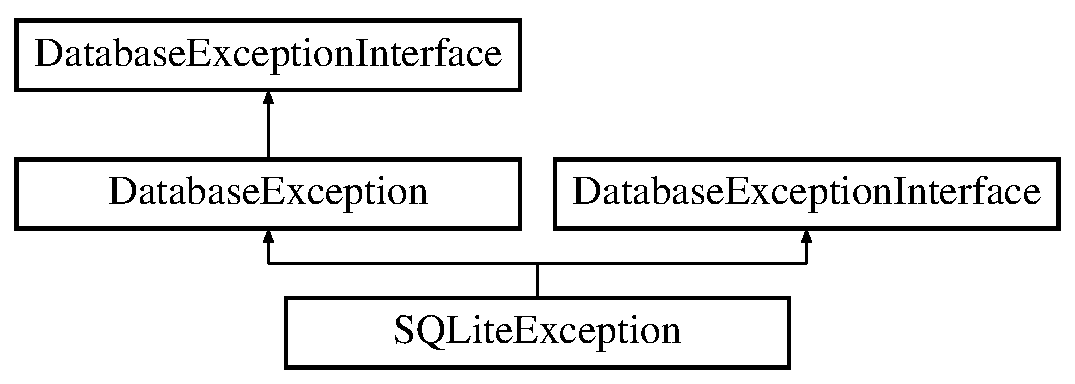
\includegraphics[height=3.000000cm]{class_s_q_lite_exception}
\end{center}
\end{figure}
\subsection*{Additional Inherited Members}


\subsection{Detailed Description}


Definition at line 3 of file S\+Q\+Lite\+Exception.\+php.



The documentation for this class was generated from the following file\+:\begin{DoxyCompactItemize}
\item 
src/class/\hyperlink{_s_q_lite_exception_8php}{S\+Q\+Lite\+Exception.\+php}\end{DoxyCompactItemize}

\chapter{File Documentation}
\hypertarget{_cross_database_interface_8php}{}\section{src/class/\+Cross\+Database\+Interface.php File Reference}
\label{_cross_database_interface_8php}\index{src/class/\+Cross\+Database\+Interface.\+php@{src/class/\+Cross\+Database\+Interface.\+php}}
\subsection*{Data Structures}
\begin{DoxyCompactItemize}
\item 
interface \hyperlink{interface_cross_database_interface}{Cross\+Database\+Interface}
\end{DoxyCompactItemize}

\hypertarget{_database_8php}{}\section{src/class/\+Database.php File Reference}
\label{_database_8php}\index{src/class/\+Database.\+php@{src/class/\+Database.\+php}}
\subsection*{Data Structures}
\begin{DoxyCompactItemize}
\item 
class \hyperlink{class_database}{Database}
\end{DoxyCompactItemize}

\hypertarget{_database_condition_interface_8php}{}\section{src/class/\+Database\+Condition\+Interface.php File Reference}
\label{_database_condition_interface_8php}\index{src/class/\+Database\+Condition\+Interface.\+php@{src/class/\+Database\+Condition\+Interface.\+php}}
\subsection*{Data Structures}
\begin{DoxyCompactItemize}
\item 
interface \hyperlink{interface_database_condition_interface}{Database\+Condition\+Interface}
\end{DoxyCompactItemize}

\hypertarget{_database_condition_model_8php}{}\section{src/class/\+Database\+Condition\+Model.php File Reference}
\label{_database_condition_model_8php}\index{src/class/\+Database\+Condition\+Model.\+php@{src/class/\+Database\+Condition\+Model.\+php}}
\subsection*{Data Structures}
\begin{DoxyCompactItemize}
\item 
class \hyperlink{class_database_condition_model}{Database\+Condition\+Model}
\end{DoxyCompactItemize}

\hypertarget{_database_exception_8php}{}\section{src/class/\+Database\+Exception.php File Reference}
\label{_database_exception_8php}\index{src/class/\+Database\+Exception.\+php@{src/class/\+Database\+Exception.\+php}}
\subsection*{Data Structures}
\begin{DoxyCompactItemize}
\item 
class \hyperlink{class_database_exception}{Database\+Exception}
\end{DoxyCompactItemize}

\hypertarget{_database_exception_interface_8php}{}\section{src/class/\+Database\+Exception\+Interface.php File Reference}
\label{_database_exception_interface_8php}\index{src/class/\+Database\+Exception\+Interface.\+php@{src/class/\+Database\+Exception\+Interface.\+php}}
\subsection*{Data Structures}
\begin{DoxyCompactItemize}
\item 
interface \hyperlink{interface_database_exception_interface}{Database\+Exception\+Interface}
\end{DoxyCompactItemize}

\hypertarget{_database_interface_8php}{}\section{src/class/\+Database\+Interface.php File Reference}
\label{_database_interface_8php}\index{src/class/\+Database\+Interface.\+php@{src/class/\+Database\+Interface.\+php}}
\subsection*{Data Structures}
\begin{DoxyCompactItemize}
\item 
interface \hyperlink{interface_database_interface}{Database\+Interface}
\end{DoxyCompactItemize}

\hypertarget{_database_utils_8php}{}\section{src/class/\+Database\+Utils.php File Reference}
\label{_database_utils_8php}\index{src/class/\+Database\+Utils.\+php@{src/class/\+Database\+Utils.\+php}}
\subsection*{Data Structures}
\begin{DoxyCompactItemize}
\item 
class \hyperlink{class_database_utils}{Database\+Utils}
\end{DoxyCompactItemize}

\hypertarget{_my_s_q_l_condition_8php}{}\section{src/class/\+My\+S\+Q\+L\+Condition.php File Reference}
\label{_my_s_q_l_condition_8php}\index{src/class/\+My\+S\+Q\+L\+Condition.\+php@{src/class/\+My\+S\+Q\+L\+Condition.\+php}}
\subsection*{Data Structures}
\begin{DoxyCompactItemize}
\item 
class \hyperlink{class_my_s_q_l_condition}{My\+S\+Q\+L\+Condition}
\end{DoxyCompactItemize}

\hypertarget{_my_s_q_l_database_8php}{}\section{src/class/\+My\+S\+Q\+L\+Database.php File Reference}
\label{_my_s_q_l_database_8php}\index{src/class/\+My\+S\+Q\+L\+Database.\+php@{src/class/\+My\+S\+Q\+L\+Database.\+php}}
\subsection*{Data Structures}
\begin{DoxyCompactItemize}
\item 
class \hyperlink{class_my_s_q_l_database}{My\+S\+Q\+L\+Database}
\end{DoxyCompactItemize}

\hypertarget{_my_s_q_l_exception_8php}{}\section{src/class/\+My\+S\+Q\+L\+Exception.php File Reference}
\label{_my_s_q_l_exception_8php}\index{src/class/\+My\+S\+Q\+L\+Exception.\+php@{src/class/\+My\+S\+Q\+L\+Exception.\+php}}
\subsection*{Data Structures}
\begin{DoxyCompactItemize}
\item 
class \hyperlink{class_my_s_q_l_exception}{My\+S\+Q\+L\+Exception}
\end{DoxyCompactItemize}

\hypertarget{_postgre_s_q_l_condition_8php}{}\section{src/class/\+Postgre\+S\+Q\+L\+Condition.php File Reference}
\label{_postgre_s_q_l_condition_8php}\index{src/class/\+Postgre\+S\+Q\+L\+Condition.\+php@{src/class/\+Postgre\+S\+Q\+L\+Condition.\+php}}
\subsection*{Data Structures}
\begin{DoxyCompactItemize}
\item 
class \hyperlink{class_postgre_s_q_l_condition}{Postgre\+S\+Q\+L\+Condition}
\end{DoxyCompactItemize}

\hypertarget{_postgre_s_q_l_database_8php}{}\section{src/class/\+Postgre\+S\+Q\+L\+Database.php File Reference}
\label{_postgre_s_q_l_database_8php}\index{src/class/\+Postgre\+S\+Q\+L\+Database.\+php@{src/class/\+Postgre\+S\+Q\+L\+Database.\+php}}
\subsection*{Data Structures}
\begin{DoxyCompactItemize}
\item 
class \hyperlink{class_postgre_s_q_l_database}{Postgre\+S\+Q\+L\+Database}
\end{DoxyCompactItemize}

\hypertarget{_postgre_s_q_l_exception_8php}{}\section{src/class/\+Postgre\+S\+Q\+L\+Exception.php File Reference}
\label{_postgre_s_q_l_exception_8php}\index{src/class/\+Postgre\+S\+Q\+L\+Exception.\+php@{src/class/\+Postgre\+S\+Q\+L\+Exception.\+php}}
\subsection*{Data Structures}
\begin{DoxyCompactItemize}
\item 
class \hyperlink{class_postgre_s_q_l_exception}{Postgre\+S\+Q\+L\+Exception}
\end{DoxyCompactItemize}

\hypertarget{_s_q_lite_condition_8php}{}\section{src/class/\+S\+Q\+Lite\+Condition.php File Reference}
\label{_s_q_lite_condition_8php}\index{src/class/\+S\+Q\+Lite\+Condition.\+php@{src/class/\+S\+Q\+Lite\+Condition.\+php}}
\subsection*{Data Structures}
\begin{DoxyCompactItemize}
\item 
class \hyperlink{class_s_q_lite_condition}{S\+Q\+Lite\+Condition}
\end{DoxyCompactItemize}

\hypertarget{_s_q_lite_database_8php}{}\section{src/class/\+S\+Q\+Lite\+Database.php File Reference}
\label{_s_q_lite_database_8php}\index{src/class/\+S\+Q\+Lite\+Database.\+php@{src/class/\+S\+Q\+Lite\+Database.\+php}}
\subsection*{Data Structures}
\begin{DoxyCompactItemize}
\item 
class \hyperlink{class_s_q_lite_database}{S\+Q\+Lite\+Database}
\end{DoxyCompactItemize}

\hypertarget{_s_q_lite_exception_8php}{}\section{src/class/\+S\+Q\+Lite\+Exception.php File Reference}
\label{_s_q_lite_exception_8php}\index{src/class/\+S\+Q\+Lite\+Exception.\+php@{src/class/\+S\+Q\+Lite\+Exception.\+php}}
\subsection*{Data Structures}
\begin{DoxyCompactItemize}
\item 
class \hyperlink{class_s_q_lite_exception}{S\+Q\+Lite\+Exception}
\end{DoxyCompactItemize}

\hypertarget{_p_h_p_d_a_l_8php}{}\section{src/\+P\+H\+P\+D\+A\+L.php File Reference}
\label{_p_h_p_d_a_l_8php}\index{src/\+P\+H\+P\+D\+A\+L.\+php@{src/\+P\+H\+P\+D\+A\+L.\+php}}
\subsection*{Namespaces}
\begin{DoxyCompactItemize}
\item 
 \hyperlink{namespace_p_h_p_d_a_l}{P\+H\+P\+D\+A\+L}
\end{DoxyCompactItemize}

%--- End generated contents ---

% Index
\backmatter
\newpage
\phantomsection
\clearemptydoublepage
\addcontentsline{toc}{chapter}{Index}
\printindex

\end{document}
